\documentclass[10pt]{beamer}
\usepackage[T1]{fontenc}
\usepackage{FiraSans} 
%\usepackage[sfdefault]{FiraSans}


%--------------------------------------------------------------------------------
%
% Choose how your presentation looks.
%
% For more themes, color themes and font themes, see:
% http://deic.uab.es/~iblanes/beamer_gallery/index_by_theme.html
%
\mode<presentation>
{
  \usetheme[progressbar=foot,numbering=fraction,background=light]{metropolis}      % or try Darmstadt, Madrid, Warsaw, ...
  \usecolortheme{default} % or try albatross, beaver, crane, ...
  \usefonttheme{default}  % or try serif, structurebold, ...
  \setbeamertemplate{navigation symbols}{}
  \setbeamertemplate{caption}[numbered]
  %\setbeamertemplate{frame footer}{My custom footer}
} 

\usepackage[ngerman,english]{babel}
\usepackage{csquotes}
%\usepackage[utf8x]{inputenc}
\usepackage{fontspec}
\usepackage{ifthen}
%--------------------------------------------------------------------------------

%--------------------------Editor mode.

%\bibliography{literature.bib}
\usepackage[backend=biber,citestyle=mla, style=authoryear]{biblatex}
\addbibresource{literature.bib} 

%\DeclareFieldFormat{postnote}{#1}\DeclareFieldFormat{multipostnote}{#1}
%\DeclareAutoCiteCommand{footnote}[f]{\footcite}{\footcites}


%--------------------------Editor mode.


%--------------------------------------------------------------------------------
%\usepackage[default]{raleway}
\usepackage{fontawesome}
%\usepackage{enumitem} % produces fatal error with this template

\usepackage{xcolor}
\definecolor{customcolor}{HTML}{616AC5}
\definecolor{alert}{HTML}{CD5C5C}
\definecolor{w3schools}{HTML}{4CAF50}
\definecolor{subbox}{gray}{0.60}
\definecolor{codecolor}{HTML}{FFC300}


%--------------------------------------------------------------------------------

\definecolor{erOrange}{HTML}{e8851c}
\definecolor{erGreen}{HTML}{129814}
\definecolor{erBlue}{HTML}{186fcb}

\usepackage{tikz}
\usetikzlibrary{er}
    \tikzset{multi attribute/.style={attribute, double distance=1.5pt},inner sep=1pt}
\tikzset{derived attribute/.style={attribute, dashed},inner sep=1pt}
\tikzset{total/.style={double distance=2.5pt},inner sep=1pt}
\tikzset{every entity/.style={draw=erBlue, fill=erBlue!20},inner sep=1pt}
\tikzset{every attribute/.style={draw=erOrange, fill=erOrange!20},inner sep=1pt}
\tikzset{every relationship/.style={draw=erGreen, fill=erGreen!20},inner sep=1pt}
\newcommand{\key}[1]{\underline{#1}}

%--------------------------------------------------------------------------------


%-------------------------------------------------------------------------------- 
%Information to be included in the title page:
\title[Data Modelling] %optional
{Information Modelling I}
\subtitle{Introduction to Data Modelling}
\institute{%Zentrum für Informationsmodellierung, Graz
}
\author[SL]{\hfill Sarah Lang}
\date[2022] % (optional)
{%Universität Graz, 
\hfill 2022%\today
}

\logo{%
\includegraphics[height=1cm]{unipassau.png}
%
\includegraphics[height=1cm]{univie-logo.png}
%
\includegraphics[height=2cm]{zim.png}
}

%--------------------------------------------------------------------------------
\newcommand{\punkti}{~\lbrack\dots\rbrack~}

\renewenvironment{quote}
               {\list{\faQuoteLeft\phantom{ }}{\rightmargin\leftmargin}%
                \item\relax\footnotesize\ignorespaces}
               {\unskip\unskip\phantom{xx}\faQuoteRight\endlist}

\newcommand{\bgupper}[3]{\colorbox{#1}{\color{#2}\huge\bfseries\MakeUppercase{#3}}}
\newcommand{\bg}[3]{\colorbox{#1}{\bfseries\color{#2}#3}}

\newcommand{\mycommand}[2]{{\ttfamily\detokenize{#1}}~\dotfill{}~{ #2}\\} % footnotesize

\newcommand{\sep}{{\scriptsize~\faCircle{ }~}}

\newcommand{\red}[1]{\bg{alert}{white}{#1}\\}
\newcommand{\green}[1]{\bg{w3schools}{white}{#1}\\}
%--------------------------------------------------------------------------------



%--------------------------------------------------------------------------------
\usepackage{xcolor}
\definecolor{customcolor}{HTML}{616AC5}
\definecolor{alert}{HTML}{CD5C5C}
\definecolor{w3schools}{HTML}{4CAF50}
\definecolor{subbox}{gray}{0.60}
\definecolor{codecolor}{HTML}{FFC300}


%--------------------------------------------------------------------------------
\usepackage{tcolorbox}

\tcbuselibrary{most,listingsutf8,minted}

\tcbset{tcbox width=auto,left=1mm,top=1mm,bottom=1mm,
right=1mm,boxsep=1mm,middle=1pt}

\newenvironment{mycolorbox}[2]{%
\begin{tcolorbox}[grow to left by=-1em,grow to right by=-1em,capture=minipage,fonttitle=\large\bfseries, enhanced jigsaw,boxsep=1mm,colback=#1!30!white,on line,tcbox width=auto, toptitle=0mm,colframe=#1,opacityback=0.7,nobeforeafter,title=#2]\scriptsize%
}{\end{tcolorbox}\\[0.2em]}

\newenvironment{subbox}[2]{%
\begin{tcolorbox}[capture=minipage,fonttitle=\normalsize\bfseries, enhanced jigsaw,boxsep=1mm,colback=#1!30!white,on line,tcbox width=auto,left=0.3em,top=1mm, toptitle=0mm,colframe=#1,opacityback=0.7,nobeforeafter,title=#2]\scriptsize %
}{\normalsize\end{tcolorbox}\vspace{0.1em}}

\newenvironment{multibox}[1]{%
\begin{tcbraster}[raster columns=#1,raster equal height,nobeforeafter,raster column skip=1em,raster left skip=1em,raster right skip=1em]}{\end{tcbraster}}


\newenvironment{mycodebox}[2]{%
\begin{tcolorbox}[grow to left by=-1em,grow to right by=-1em,capture=minipage,fonttitle=\large\bfseries, enhanced jigsaw,boxsep=1mm,colback=#1!30!white,on line,tcbox width=auto, toptitle=0mm,colframe=#1,opacityback=0.7,nobeforeafter,title=#2]%
}{\end{tcolorbox}\\[0.2em]}

\newtcolorbox{mybox}[2][]{colback=codecolor!10!white,coltitle=red!70!black,
title={#2},fonttitle=\bfseries,#1}


%-------------------------------

\newtcblisting{mypy}[1]{colback=codecolor!5,colframe=codecolor!80!black,listing only, 
minted options={numbers=left, style=tcblatex,fontsize=\scriptsize,breaklines,autogobble,linenos,numbersep=3mm},
left=5mm,enhanced,
title=#1, fonttitle=\bfseries,
listing engine=minted,minted language=python}

\newtcblisting{myxml}[1]{colback=codecolor!5,colframe=codecolor!80!black,listing only, 
minted options={numbers=left, style=tcblatex,fontsize=\tiny,breaklines,autogobble,linenos,numbersep=3mm},
left=5mm,enhanced,
title=#1, fonttitle=\bfseries,
listing engine=minted,minted language=xml}

\newtcblisting{mybiggerxml}[1]{colback=codecolor!5,colframe=codecolor!80!black,listing only,
minted options={numbers=left, style=tcblatex,fontsize=\footnotesize,breaklines,autogobble,linenos,numbersep=3mm},
left=5mm,enhanced,
title=#1, fonttitle=\bfseries,
listing engine=minted,minted language=xml}

\newtcblisting{myhtml}[1]{colback=codecolor!5,colframe=codecolor!80!black,listing only, 
minted options={numbers=left, style=tcblatex,fontsize=\tiny,breaklines,autogobble,linenos,numbersep=3mm},
left=5mm,enhanced,
title=#1, fonttitle=\bfseries,
listing engine=minted,minted language=html}


\newtcblisting{mycss}[1]{colback=codecolor!5,colframe=codecolor!80!black,listing only, 
minted options={numbers=left, style=tcblatex,fontsize=\tiny,breaklines,autogobble,linenos,numbersep=3mm},
left=5mm,enhanced,
title=#1, fonttitle=\bfseries,
listing engine=minted,minted language=css}


\newtcblisting{myjs}[1]{colback=codecolor!5,colframe=codecolor!80!black,listing only, 
minted options={numbers=left, style=tcblatex,fontsize=\tiny,breaklines,autogobble,linenos,numbersep=3mm},
left=5mm,enhanced,
title=#1, fonttitle=\bfseries,
listing engine=minted,minted language=js}


\newtcblisting{mysql}[1]{colback=codecolor!5,colframe=codecolor!80!black,listing only, 
minted options={numbers=left, style=tcblatex,fontsize=\tiny,breaklines,autogobble,linenos,numbersep=3mm},
left=5mm,enhanced,
title=#1, fonttitle=\bfseries,
listing engine=minted,minted language=sql}

% black!5 ist auch nicht so ganz schlecht, aber sehr hell; black!8; black!10
\newtcblisting{greysql}{colback=black!8,colframe=black!8,listing only, 
minted options={numbers=left, style=tcblatex,fontsize=\tiny,breaklines,autogobble,linenos,numbersep=3mm},
left=5mm,enhanced, fonttitle=\bfseries,
listing engine=minted,minted language=sql}

\definecolor{bgcolour}{rgb}{0.95,0.95,0.95}
\newminted{sql}{fontsize=\footnotesize, 
                   linenos,
                   %fontfamily=fi4, 
                   numbersep=6pt,
                   autogobble,
                   %frame=lines,
                   bgcolor=black!8,
                   framesep=3mm} 

%\usemintedstyle[shell-session]{vim} %  vim monokai fruity native
% color=black!80
\newminted{shell-session}{fontsize=\scriptsize,numbersep=6pt,bgcolor=black!70,autogobble,framesep=3mm%  %frame=lines, %fontfamily=fi4, 
                   }                    
                   
\newminted{sparql}{fontsize=\scriptsize, 
                   %linenos,
                   %fontfamily=fi4, 
                   numbersep=6pt,
                   autogobble,
                   %frame=lines,
                   bgcolor=black!8,
                   framesep=3mm} 
                   
\newminted{turtle}{fontsize=\scriptsize, 
                   %linenos,
                   %fontfamily=fi4, 
                   numbersep=6pt,
                   autogobble,
                   %frame=lines,
                   bgcolor=black!8,
                   framesep=3mm} 
                   
\newminted{js}{fontsize=\scriptsize, 
                   linenos,
                   %fontfamily=fi4, 
                   numbersep=6pt,
                   autogobble,
                   %frame=lines,
                   bgcolor=black!8,
                   framesep=3mm}                    

\newminted{xml}{fontsize=\scriptsize, 
                   %linenos,
                   %fontfamily=fi4, 
                   numbersep=6pt,
                   autogobble,
                   %frame=lines,
                   bgcolor=black!8,
                   framesep=3mm} 
\newminted{html}{fontsize=\scriptsize, 
                   %linenos,
                   %fontfamily=fi4, 
                   numbersep=6pt,
                   autogobble,
                   %frame=lines,
                   bgcolor=black!8,
                   framesep=3mm} 
                   
\newminted{css}{fontsize=\scriptsize, 
                   %linenos,
                   %fontfamily=fi4, 
                   numbersep=6pt,
                   autogobble,
                   %frame=lines,
                   bgcolor=black!8,
                   framesep=3mm} 
                   
\newminted{postscript}{fontsize=\scriptsize, 
                   %linenos,
                   %fontfamily=fi4, 
                   numbersep=6pt,
                   autogobble,
                   %frame=lines,
                   bgcolor=black!8,
                   framesep=3mm}                    
                 
                   
%-------------------------------  
% https://tex.stackexchange.com/questions/377777/why-do-my-beamer-blocks-without-title-still-have-a-background
\usepackage{xstring}                
\setbeamertemplate{block begin}
{
  \par\vskip\medskipamount%
  \IfStrEq{\insertblocktitle}{}{}{
      \begin{beamercolorbox}[colsep*=.75ex]{block title}
        \usebeamerfont*{block title}\insertblocktitle%
      \end{beamercolorbox}%
  }
  {\parskip0pt\par}%
  \ifbeamercolorempty[bg]{block title}
  {}
  {\ifbeamercolorempty[bg]{block body}{}{\nointerlineskip\vskip-0.5pt}}%
  \usebeamerfont{block body}%
  \begin{beamercolorbox}[colsep*=.75ex,vmode]{block body}%
    \ifbeamercolorempty[bg]{block body}{\vskip-.25ex}{\vskip-.75ex}\vbox{}%
}
%-------------------------------  


\usepackage{multicol}
\usepackage{hyperref}
%%--------------------------------------------------------------------------------
\usepackage{graphicx}
\usepackage{tikz}
%--------------------------------------------------------------------------------
% Uni Graz Corporate Font has to be Franklin Gothic
\usepackage{librefranklin}
\renewcommand*\familydefault{\sfdefault} %% Only if the base font of the document is to be sans serif

% font for base text \setmainfont{librefranklin}
 
% font for title  -\setbeamerfont{title}{family=\fontspec{librefranklin}}
 
% for other elements on title page (author, date) \setbeamerfont{title page}{family=\fontspec{librefranklin}}

%--------------------------------------------------------------------------------
\pgfdeclareimage[width=\paperwidth]{mybackground}{img/kfu-zim-slides.png}

\setbeamertemplate{title page}{
  \begin{minipage}[b][\paperheight]{\textwidth}
              \put(-30,-163){%
                \pgfuseimage{mybackground}
            }
    \ifx\inserttitlegraphic\@empty\else\usebeamertemplate*{title graphic}\fi
    \vfill%
    \ifx\inserttitle\@empty\else\usebeamertemplate*{title}\fi
    \ifx\insertsubtitle\@empty\else\usebeamertemplate*{subtitle}\fi
    \usebeamertemplate*{title separator}
    \ifx\beamer@shortauthor\@empty\else\usebeamertemplate*{author}\fi
    \ifx\insertdate\@empty\else\usebeamertemplate*{date}\fi
    \ifx\insertinstitute\@empty\else\usebeamertemplate*{institute}\fi
    \vfill
    \vspace*{1mm}
  \end{minipage}
}

%--------------------------------------------------------------------------------

 
\begin{document}

%------------------------------------------------------------------------------
% FRONT
%------------------------------------------------------------------------------

{
\usebackgroundtemplate{
\includegraphics[width=\paperwidth]{img/kfu-zim-slides.png}}
\frame{\titlepage}
}
%\frame{\titlepage}

%------------------------------------------------------------------------------
\begin{frame}{}%\scriptsize
  \setbeamertemplate{section in toc}[sections numbered]
  \begin{small}
  \begin{multicols}{2}\tableofcontents\end{multicols}
  % on toc formatting:
  % https://tex.stackexchange.com/questions/26929/two-column-beamer-toc-with-control-over-the-breaking-point
  \end{small}
\end{frame}

\metroset{block=fill}
\section{Syllabus}
%------------------------------------------------------------------------------
\begin{frame}{Content}
Theoretical and practical introduction to modelling data in tabular formats. 

\begin{enumerate}
    \item tabular data
    \item relational model (Entity-Relationship-Model) 
    \item SQL databases
\end{enumerate}

\end{frame}
 
\section{Preliminaries}
%------------------------------------------------------------------------------
\begin{frame}{How to get a positive grade on this class}
\subsection{Grading}

  \begin{columns}[T,onlytextwidth]
    \column{0.48\textwidth}
      \begin{exampleblock}{Final Submission (60\%)}
\begin{itemize}\footnotesize
\item \textbf{Infomod:} Text, ER model, SQL database
\item \textbf{DigEd:} Small digital edition or review of an existing edition.
\item You can start in the last month of the semester and ask questions.
\item You can collaborate but no plagiarism (Uni Graz zero tolerance policy).
\end{itemize}
\end{exampleblock}

\begin{exampleblock}{Homework assignments (40\%)}\footnotesize
Communicated and to be completed within the week
\end{exampleblock}

    \column{0.48\textwidth}
      \begin{alertblock}{Other aspects}
\begin{enumerate}\scriptsize
    \item attendance in class (you can miss max. 3, to be communicated beforehand).
    \item Positive grade: at least 50\%  on all partial submissions.
    \item ``LVen mit immanentem Prüfungscharakter'' $\to$ once you accept the first task you get a grade (i.e. first homework this week)
    \item If you get a negative grade, the whole class needs to be retaken.
\end{enumerate}

\begin{quote}\scriptsize
    Nichterbringung weiterer Teilleistungen ohne wichtigen Grund ist Prüfungsabbruch (Negativbeurteilung). Abmeldung nach bereits übernommener Teilleistung führt zu negativer Beurteilung.
\end{quote}
\end{alertblock}

\end{columns}

\small 
see also: slides on grading \& further info materials on the final submission
    
\end{frame}


%------------------------------------------------------------------------------
\begin{frame}{Deadlines}

\begin{alertblock}{Hard deadlines}\small
\textbf{All deadlines are hard deadlines.} 
You can get extensions for good reasons.
\begin{itemize}
\item Good reasons for example: care responsibility, being ill, etc.
\item i.e. understandable reasons which are communicated asap
\end{itemize}
\end{alertblock}

\begin{alertblock}{If you miss a deadline\dots}
\begin{itemize}\small
\item If you didn’t communicate: negative grade.
\item Otherwise up for discussion according to the circumstances.
\end{itemize}
\end{alertblock}

\end{frame}
%------------------------------------------------------------------------------
\begin{frame}{Learning Goals}
\subsection{Learning Goals}
\begin{enumerate}
    \item get to know modelling theory („Allgemeine Modelltheorie“ nach Herbert Stachowiak)
    \begin{itemize}
        \item try the Entity-Relationship-Diagramm (Peter Chen)
        \item go from conceptual model to computer processable model
        \item represent relational data structures
    \end{itemize}
    \item learn SQL (\emph{Structured Query Language})
    \item get to know different data structures 
    \item basic practical modelling experience
\end{enumerate}

\metroset{block=fill}
\begin{alertblock}{Final project}
\footnotesize
Move from your own conceptual data model to a relational database in SQL and write about it (3--5 pages). 

\end{alertblock}
\end{frame}

%------------------------------------------------------------------------------
\begin{frame}{Literature on learning tech subjects}

\begin{enumerate}
    \item Carol Dweck, \emph{Mindset: The New Psychology of Success} (New York: Random House 2006). {\footnotesize (\href{https://www.youtube.com/watch?v=hiiEeMN7vbQ}{10min Video } | \href{https://latex-ninja.com/2021/06/21/the-most-important-book-to-read-if-you-want-to-learn-digital-humanities-computer-science-maths-programming-or-latex/}{blog post on the topic}) }
    \item K. Anders Ericsson \& Robert Pool, \emph{Peak: Secrets from the New Science of Expertise}, Penguin: London 2016. 
    \item Barbara Oakley, \emph{A Mind for Numbers}, NY 2014.
\end{enumerate}

\end{frame}
%------------------------------------------------------------------------------
%------------------------------------------------------------------------------
\begin{frame}{Working with computers as a humanities person}

\begin{itemize}
    \item \href{https://static.uni-graz.at/fileadmin/gewi-zentren/Informationsmodellierung/PDF/U__bungsblatt-0.pdf}{Übungsblatt 0} is a prerequisite
    \item don't panic
\end{itemize}
    
\end{frame}
%------------------------------------------------------------------------------

%------------------------------------------------------------------------------
\begin{frame}[standout]
    \alert{Present yourselves! } \\
    Name, pronouns, domain of origin, interests, etc.
\end{frame}


%------------------------------------------------------------------------------
%\begin{frame}[standout]    Resources\end{frame}
\subsection{Resources}
%------------------------------------------------------------------------------
\begin{frame}{References}
\begin{enumerate}
    \item \textbf{Stachowiak,} Herbert: \emph{Allgemeine Modelltheorie}, Wien 1973. 
    \item \textbf{Chen,} Peter: \emph{The Entity-Relationship Model -- Toward a Unified View of Data}, 1976.
    \item \textbf{Jannidis (Hg.):} \emph{Digital Humanities. Eine Einführung}, Stuttgart 2017. \\
    \begin{itemize}
        \item \href{https://link.springer.com/book/10.1007/978-3-476-05446-3}{Online-Exemplar} $\to$ gedrucktes Exemplar in der ZIM-Bibliothek.
        \item Kap. 7 (\emph{Datenmodellierung}) und 8 (\emph{Datenbanken}).
    \end{itemize}
    \item \textbf{Flanders, Julia; Jannidis, Fotis:} \emph{Knowledge Organization and Data Modeling in the Humanities}, 2015. 
    \item \textbf{Lothar Piepmeyer:} Grundkurs Datenbanksysteme. Von den Konzepten bis zur Anwendungsentwicklung, Hanser 2011. 
    \item \textbf{Ciula, Arianna \& Eide, Øyvind \& Marras, Cristina \& Sahle, Patrick (Ed.):} \emph{Models and Modelling between Digital and Humanities: A Multidisciplinary Perspective}, 2018.
    \item \textbf{Julia Flanders, Fotis Jannidis:} \emph{The Shape of Data in Digital Humanities Modeling Texts and Text-based Resources}, Routledge 2019.
\end{enumerate}

\end{frame}


%------------------------------------------------------------------------------
\begin{frame}{Ressources}

\begin{enumerate}
    \item \textbf{OpenRefine:}
    \begin{itemize}
        \item \href{https://openrefine.org/download.html\#openrefine-32}{OpenRefine Download}
        \item \href{https://openrefine.org/}{OpenRefine site with tutorials}
    \end{itemize}
    \item \textbf{SQL:}
    \begin{itemize}
        \item \href{https://sqlite.org/download.html}{SQLite Download}
        \item \href{https://sqlitebrowser.org/dl/}{SQLite Browser}
        \item \href{https://www.w3schools.com/sql/}{w3schools SQL Tutorial}
    \end{itemize}
    \item \textbf{ER:}
    \begin{itemize}
        \item \href{https://erdplus.com/standalone}{ERDplus Tool for creating ER models}
        \item \href{https://www.geeksforgeeks.org/introduction-of-er-model/}{GeeksforGeeks-Tutorial/Intro to ER Models}
    \end{itemize}
\end{enumerate}

\end{frame}


% EXAMPLES - don't include
%\section{Modelle}

\begin{frame}{Modelle in der Wissenschaft}
\begin{block}{Remark}
Sample text
\end{block}

\begin{alertblock}{Important theorem}
Sample text in red box
\end{alertblock}

\begin{examples}
Sample text in green box. The title of the block is ``Examples".
\end{examples}
    
\end{frame}


\begin{frame}{Lists}
  \begin{columns}[T,onlytextwidth]
    \column{0.33\textwidth}
      Items
      \begin{itemize}
        \item Milk \item Eggs \item Potatos
      \end{itemize}

    \column{0.33\textwidth}
      Enumerations
      \begin{enumerate}
        \item First, \item Second and \item Last.
      \end{enumerate}

    \column{0.33\textwidth}
      Descriptions
      \begin{description}
        \item[PowerPoint] Meeh. \item[Beamer] Yeeeha.
      \end{description}
  \end{columns}
\end{frame}

\begin{frame}{Modelle in der Wissenschaft}
    \begin{quote}
        In den Wissenschaften werden Modelle aus den unterschiedlichsten Gründen zur Originalrepräsentation herangezogen.~\parencite[138]{stachowiak}
    \end{quote}
    % ----------------------------------------------
  \begin{columns}[T,onlytextwidth]
  \metroset{block=fill}
    \column{0.3\textwidth}
      \begin{block}{Default}
            \begin{quote}
        In den Wissenschaften werden Modelle aus den unterschiedlichsten Gründen zur Originalrepräsentation herangezogen.~\parencite[138]{stachowiak}
    \end{quote}
      \end{block}

      \begin{alertblock}{Alert}
        Block content.
      \end{alertblock}

      \begin{exampleblock}{Example}
        Block content.
      \end{exampleblock}
    % ----------------------------------------------
    \column{0.3\textwidth}

      \metroset{block=fill}

      \begin{block}{Default}
        Block content.
      \end{block}

      \begin{alertblock}{Alert}
        Block content.
      \end{alertblock}

      \begin{exampleblock}{Example}
        Block content.
      \end{exampleblock}
      
    % ----------------------------------------------
    \column{0.3\textwidth}

      \metroset{block=fill}

      \begin{block}{Default}
        Block content.
      \end{block}

      \begin{alertblock}{Alert}
        Block content.
      \end{alertblock}

      \begin{exampleblock}{Example}
        Block content.
      \end{exampleblock}
  \end{columns}
\end{frame}


\section{Blocks Columns}
\begin{frame}{Blocks}
  Three different block environments are pre-defined and may be styled with an
  optional background color.

  \begin{columns}[T,onlytextwidth]
    \column{0.5\textwidth}
      \begin{block}{Default}
        Block content.
      \end{block}

      \begin{alertblock}{Alert}
        Block content.
      \end{alertblock}

      \begin{exampleblock}{Example}
        Block content.
      \end{exampleblock}

    \column{0.5\textwidth}

      \metroset{block=fill}

      \begin{block}{Default}
        Block content.
      \end{block}

      \begin{alertblock}{Alert}
        Block content.
      \end{alertblock}

      \begin{exampleblock}{Example}
        Block content.
      \end{exampleblock}

  \end{columns}
\end{frame}

\section{SQL-CodeSlides}
\begin{frame}[fragile]{SQL}
just minted sql
\begin{minted}{sql}
SELECT DISTINCT column_list
FROM table_list
    JOIN table ON join_condition
WHERE row_filter
ORDER BY column
LIMIT count OFFSET offset
GROUP BY column
HAVING group_filter;
\end{minted}
\end{frame}


\begin{frame}[fragile]{Test}
sqlcode  

\begin{sqlcode}
SELECT DISTINCT column_list
FROM table_list
    JOIN table ON join_condition
WHERE row_filter
ORDER BY column
LIMIT count OFFSET offset
GROUP BY column
HAVING group_filter;
\end{sqlcode}

\end{frame}


\begin{frame}[fragile]{Test}
htmlcode  

\begin{htmlcode}
<html>
<head>
<meta http-equiv="Content-Type" 
   content="text/html; charset=UTF-8">
<meta http-equiv="Content-Language" 
\end{htmlcode}

\end{frame}

%------------------------------------------------------------------------------
\begin{frame}[fragile]{Blocks}
TEST
  \begin{columns}[T,onlytextwidth]
    \column{0.5\textwidth}
      \begin{itemize}
          \item info
      \end{itemize}
      
      \begin{block}{Default}
        Block content.
      \end{block}

      \begin{alertblock}{Alert}
        Block content.
      \end{alertblock}

      \begin{exampleblock}{Example}
        Block content.
      \end{exampleblock}

    \column{0.5\textwidth}
      \begin{greysql}
SELECT DISTINCT column_list
FROM table_list
    JOIN table ON join_condition
WHERE row_filter
ORDER BY column
LIMIT count OFFSET offset
GROUP BY column
HAVING group_filter;
\end{greysql}

  \end{columns}
\end{frame}

%------------------------------------------------------------------------------
\begin{frame}[fragile]{Blocks}
  Three different block environments are pre-defined and may be styled with an
  optional background color.

  \begin{columns}[T,onlytextwidth]
    \column{0.4\textwidth}
      \begin{itemize}
          \item info
      \end{itemize}
      
      \begin{block}{Default}
        Block content.
      \end{block}

      \begin{alertblock}{Alert}
        Block content.
      \end{alertblock}

      \begin{exampleblock}{Example}
        Block content.
      \end{exampleblock}

    \column{0.6\textwidth}
\begin{sqlcode}
SELECT DISTINCT column_list
FROM table_list
    JOIN table ON join_condition
WHERE row_filter
ORDER BY column
LIMIT count OFFSET offset
GROUP BY column
HAVING group_filter;
\end{sqlcode}

  \end{columns}
\end{frame}

\section{Modelle nochmal}
%------------------------------------------------------------------------------
\begin{frame}{Modelle in der Wissenschaft}
    \begin{quote}
        In den Wissenschaften werden Modelle aus den unterschiedlichsten Gründen zur Originalrepräsentation herangezogen.~\parencite[138]{stachowiak}
    \end{quote}
    \begin{quote}
        Als Demonstrationsmodelle werden sie zur
Veranschaulichung von (weniger anschaulichen oder
unanschaulichen) Zusammenhängen benutzt, \punkti.~\parencite[138]{stachowiak}
    \end{quote}
    % ----------------------------------------------
  \begin{columns}[T,onlytextwidth]
  %\metroset{block=fill}
    \column{0.5\textwidth}
      \begin{block}{Default}
            \begin{quote}
        In den Wissenschaften werden Modelle aus den unterschiedlichsten Gründen zur Originalrepräsentation herangezogen.~\parencite[138]{stachowiak}
    \end{quote}
      \end{block}

      \begin{alertblock}{Alert}
        Block content.
      \end{alertblock}

      \begin{exampleblock}{Example}
        Block content.
      \end{exampleblock}
    % ----------------------------------------------

    \column{0.5\textwidth}

      \metroset{block=transparent}

      \begin{block}{Demonstrationsmodelle}
            \begin{quote}
        Als Demonstrationsmodelle werden sie zur
Veranschaulichung von (weniger anschaulichen oder
unanschaulichen) Zusammenhängen benutzt, \punkti.~\parencite[138]{stachowiak}
    \end{quote}
      \end{block}

      \begin{alertblock}{Alert}
        Block content.
      \end{alertblock}

      \begin{exampleblock}{Example}
        Block content.
      \end{exampleblock}

  \end{columns}
\end{frame}


%------------------------------------------------------------------------------
\begin{frame}{Modelltheorie Fortsetzung}
Grundlagen der Datenmodellierung
\begin{itemize}\small
    \item Daten
    \item Modellierung 
    \item Modelle
\end{itemize}
\begin{columns}[T,onlytextwidth]
\column{0.45\textwidth}

\metroset{block=fill}
    \begin{block}{\cite[131]{stachowiak}}
        \begin{quote}
        
        \end{quote}
    \end{block}
\begin{exampleblock}{\footnotesize Welche Informationen bzw. welches (abstrakte) Wissen steckt im Globus bzw. in Google Maps/Google Earth? }
    \begin{itemize}\footnotesize
        \item 
    \end{itemize}
\end{exampleblock}
% Aus welchen Gründen bzw. zu welchem Zweck könnten die Modelle zur Originalrepräsentation herangezogen werden?

\column{0.5\textwidth}
\begin{alertblock}{Wozu?}
\begin{enumerate}\small
    \item 
\end{enumerate}
\end{alertblock}

\begin{alertblock}{Wie? (Operationen mit dem Modell)}
\begin{enumerate}\small
    \item 
\end{enumerate}
\end{alertblock}
\end{columns}

\end{frame}


%------------------------------------------------------------------------------
\begin{frame}{Operative Modelle}
  \begin{columns}[T,onlytextwidth]
  \metroset{block=fill}
    \column{0.5\textwidth}
    
    \begin{quote} 
    \end{quote}
    % ----------------------------------------------
    \column{0.5\textwidth}
    \metroset{block=fill}
        \begin{block}{\cite[131]{stachowiak}}
        \begin{quote}
            
        \end{quote}
    \end{block}
    \metroset{block=fill}
      \begin{block}{\footnotesize Modellbildung Bsp. Globus}
      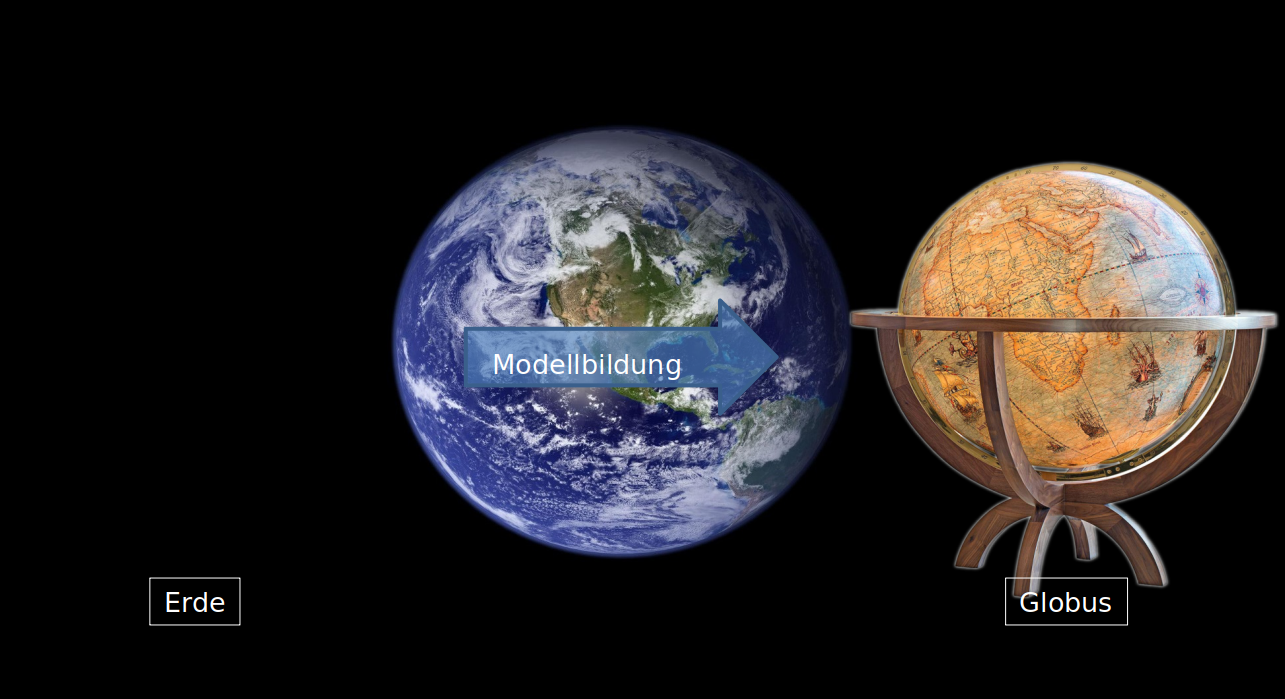
\includegraphics[width=0.95\textwidth]{img/modell-globus2.png}
      \end{block}

  \end{columns}

\begin{columns}[T,onlytextwidth]

\column{0.3\textwidth}

\column{0.3\textwidth}

\column{0.3\textwidth}

\end{columns}
\end{frame}
%------------------------------------------------------------------------------
\begin{frame}{Experimentalmodelle}
    \begin{quote}
„\punkti als Experimentalmodelle dienen sie der Ermittlung
oder Überprüfung von Hypothesen \punkti“~\parencite[139]{stachowiak}
    \end{quote}
    \begin{quote}
        Als Demonstrationsmodelle werden sie zur
Veranschaulichung von (weniger anschaulichen oder
unanschaulichen) Zusammenhängen benutzt, \punkti.~\parencite[138]{stachowiak}
    \end{quote}
    % ----------------------------------------------
  \begin{columns}[T,onlytextwidth]
  \metroset{block=fill}
    \column{0.3\textwidth}
      \begin{block}{Default}
      \href{https://youtu.be/K0aPuLn76H0}{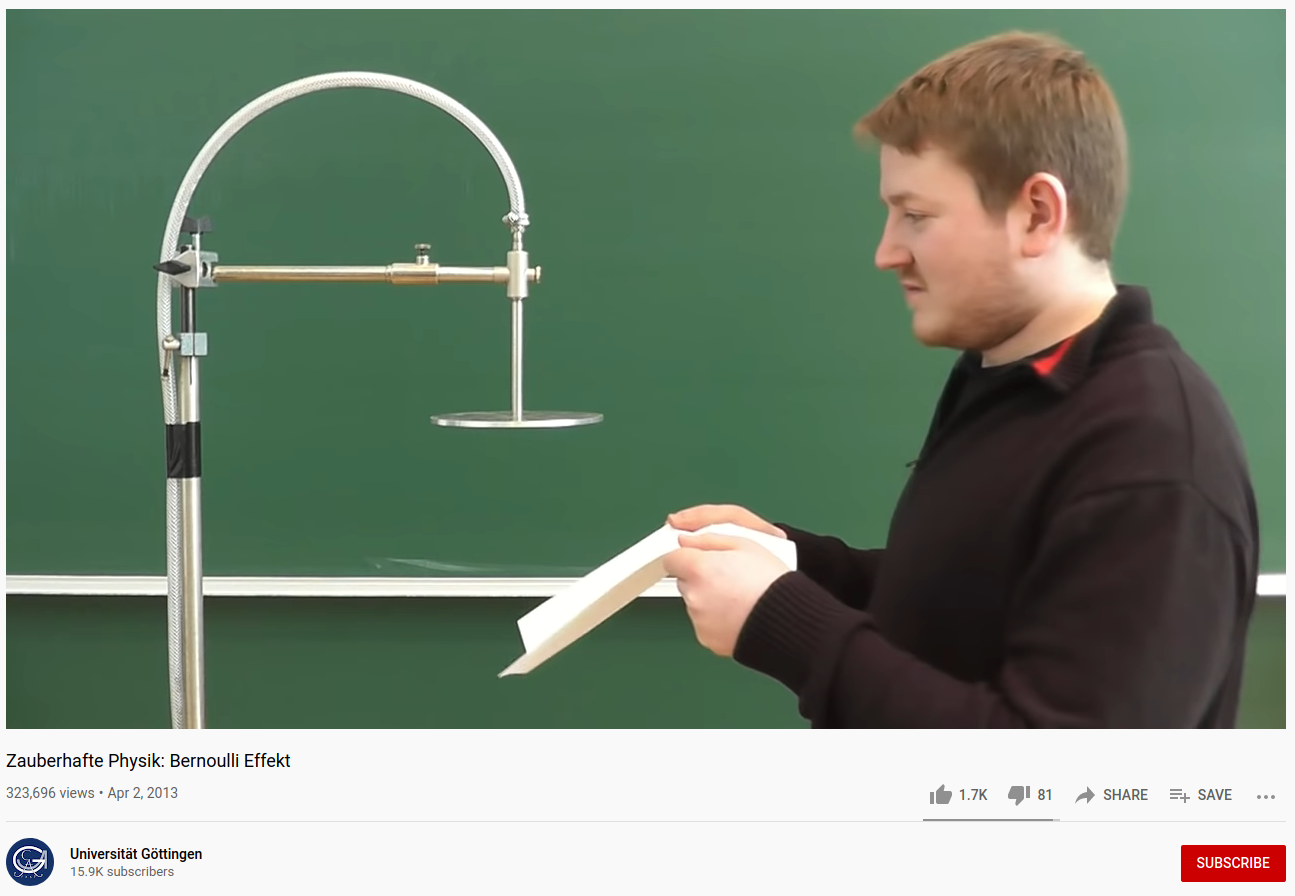
\includegraphics[width=0.3\textwidth]{img/physik-bernoulli.png}}
      \end{block}

      \begin{alertblock}{Alert}
        Block content.
      \end{alertblock}

      \begin{exampleblock}{Example}
        Block content.
      \end{exampleblock}
    % ----------------------------------------------
    \column{0.3\textwidth}

      \metroset{block=fill}

      \begin{block}{Default}
        Block content.
      \end{block}

      \begin{alertblock}{Alert}
        Block content.
      \end{alertblock}

      \begin{exampleblock}{Example}
        Block content.
      \end{exampleblock}
      
    % ----------------------------------------------
    \column{0.3\textwidth}

      \metroset{block=fill}

      \begin{block}{Default}
        Block content.
      \end{block}

      \begin{alertblock}{Alert}
        Block content.
      \end{alertblock}

      \begin{exampleblock}{Example}
        Block content.
      \end{exampleblock}
  \end{columns}
\end{frame}

{\setbeamercolor{palette primary}{fg=black, bg=yellow}
\begin{frame}[standout]
  Questions?
\end{frame}
}

\appendix

\begin{frame}[fragile]{Backup slides}
  Sometimes, it is useful to add slides at the end of your presentation to
  refer to during audience questions.

  The best way to do this is to include the \verb|appendixnumberbeamer|
  package in your preamble and call \verb|\appendix| before your backup slides.

  \themename will automatically turn off slide numbering and progress bars for
  slides in the appendix.
\end{frame}

\begin{frame}[allowframebreaks]{References}

  \bibliography{demo}
  \bibliographystyle{abbrv}

\end{frame}





%------------------------------------------------------------------------------
\begin{frame}[fragile]{Blocks}
  Three different block environments are pre-defined and may be styled with an
  optional background color.

  \begin{columns}[T,onlytextwidth]
    \column{0.4\textwidth}
      \begin{itemize}
          \item info
      \end{itemize}
      
      \begin{block}{Default}
        Block content.
      \end{block}

      \begin{alertblock}{Alert}
        Block content.
      \end{alertblock}

      \begin{exampleblock}{Example}
        Block content.
      \end{exampleblock}

    \column{0.6\textwidth}
\begin{sqlcode}
SELECT DISTINCT column_list
FROM table_list
    JOIN table ON join_condition
WHERE row_filter
ORDER BY column
LIMIT count OFFSET offset
GROUP BY column
HAVING group_filter;
\end{sqlcode}

  \end{columns}
\end{frame}


%------------------------------------------------------------------------------
\begin{frame}[fragile]{Blocks}
  Three different block environments are pre-defined and may be styled with an
  optional background color.

  \begin{columns}[T,onlytextwidth]
    \column{0.5\textwidth}
      \begin{itemize}
          \item info
      \end{itemize}
      
      \begin{block}{Default}
        Block content.
      \end{block}

      \begin{alertblock}{Alert}
        Block content.
      \end{alertblock}

      \begin{exampleblock}{Example}
        Block content.
      \end{exampleblock}

    \column{0.5\textwidth}
      \begin{greysql}
SELECT DISTINCT column_list
FROM table_list
    JOIN table ON join_condition
WHERE row_filter
ORDER BY column
LIMIT count OFFSET offset
GROUP BY column
HAVING group_filter;
\end{greysql}

  \end{columns}
\end{frame}


%------------------------------------------------------------------------------
\begin{frame}{Blocks}
  Three different block environments are pre-defined and may be styled with an
  optional background color.

  \begin{columns}[T,onlytextwidth]
    \column{0.5\textwidth}
      \begin{block}{Default}
        Block content.
      \end{block}

      \begin{alertblock}{Alert}
        Block content.
      \end{alertblock}

      \begin{exampleblock}{Example}
        Block content.
      \end{exampleblock}

    \column{0.5\textwidth}

      \metroset{block=fill}

      \begin{block}{Default}
        Block content.
      \end{block}

      \begin{alertblock}{Alert}
        Block content.
      \end{alertblock}

      \begin{exampleblock}{Example}
        Block content.
      \end{exampleblock}

  \end{columns}
\end{frame}

%------------------------------------------------------------------------------
\begin{frame}[fragile]{Blocks}
TEST
  \begin{columns}[T,onlytextwidth]
    \column{0.5\textwidth}
      \begin{itemize}
          \item info
      \end{itemize}
      
      \begin{block}{Default}
        Block content.
      \end{block}

      \begin{alertblock}{Alert}
        Block content.
      \end{alertblock}

      \begin{exampleblock}{Example}
        Block content.
      \end{exampleblock}

    \column{0.5\textwidth}
      \begin{greysql}
SELECT DISTINCT column_list
FROM table_list
    JOIN table ON join_condition
WHERE row_filter
ORDER BY column
LIMIT count OFFSET offset
GROUP BY column
HAVING group_filter;
\end{greysql}

  \end{columns}
\end{frame}

%------------------------------------------------------------------------------
\begin{frame}[fragile]{Blocks}
  Three different block environments are pre-defined and may be styled with an
  optional background color.

  \begin{columns}[T,onlytextwidth]
    \column{0.4\textwidth}
      \begin{itemize}
          \item info
      \end{itemize}
      
      \begin{block}{Default}
        Block content.
      \end{block}

      \begin{alertblock}{Alert}
        Block content.
      \end{alertblock}

      \begin{exampleblock}{Example}
        Block content.
      \end{exampleblock}

    \column{0.6\textwidth}
\begin{sqlcode}
SELECT DISTINCT column_list
FROM table_list
    JOIN table ON join_condition
WHERE row_filter
ORDER BY column
LIMIT count OFFSET offset
GROUP BY column
HAVING group_filter;
\end{sqlcode}


\begin{columns}
  \column{0.45\textwidth}
  \column{0.55\textwidth}
\end{columns}
  

  \end{columns}
\end{frame}








%------------------------------------------------------------------------------
% MAIN
%------------------------------------------------------------------------------
%\section{Einführung}

\section{Modelling theory: Models in research}
%------------------------------------------------------------------------------
\begin{frame}{Models in research}

    % ----------------------------------------------
  \begin{columns}%[T,onlytextwidth]
  %\metroset{block=fill}
    \column{0.45\textwidth}
        \begin{quote}
        In den Wissenschaften werden Modelle aus den unterschiedlichsten Gründen zur Originalrepräsentation herangezogen.~\parencite[138]{stachowiak}
    \end{quote}
    \bigskip
    
    \begin{itemize}
        \item demonstration models
        \item experimental models
        \item theoretical models
        \item operative models
    \end{itemize}
    \bigskip
    
    \footnotesize
    
    For English summary of Stachowiak see: \protect\url{https://modelpractice.wordpress.com/2012/07/04/model-stachowiak/}
    % ----------------------------------------------

    \column{0.55\textwidth}

      \metroset{block=fill} % transparent

      \begin{alertblock}{All knowledge production happens in the context of models}
        \begin{quote}
Der Gewinn dieser Vorgehensweise \lbrack{}Modellierung\rbrack{} liegt
auf der Hand: Modellseitig gewonnene Einsichten und
Fertigkeiten lassen sich -- bei Erfülltsein gewisser
Transferierungskriterien -- auf das Original übertragen,
der Modellbildner gewinnt neue Kenntnisse über das
modellierte Original, er bekommt dieses besser als
bisher in den Griff, kann es auf neue Weise
zweckdienlich umgestalten oder als verbessertes
Hilfsmittel für neue Aktionen verwenden.~\parencite[140]{stachowiak}
        \end{quote}
      \end{alertblock}
  \end{columns}
\end{frame}

%------------------------------------------------------------------------------
\begin{frame}{Demonstration models}
  \begin{columns}%[T,onlytextwidth]
  \metroset{block=fill}
    \column{0.5\textwidth}
         \begin{quote}
        Als Demonstrationsmodelle werden sie zur
Veranschaulichung von (weniger anschaulichen oder
unanschaulichen) Zusammenhängen benutzt, \punkti.~\parencite[138]{stachowiak}
    \end{quote}\bigskip
    
    {\hfill 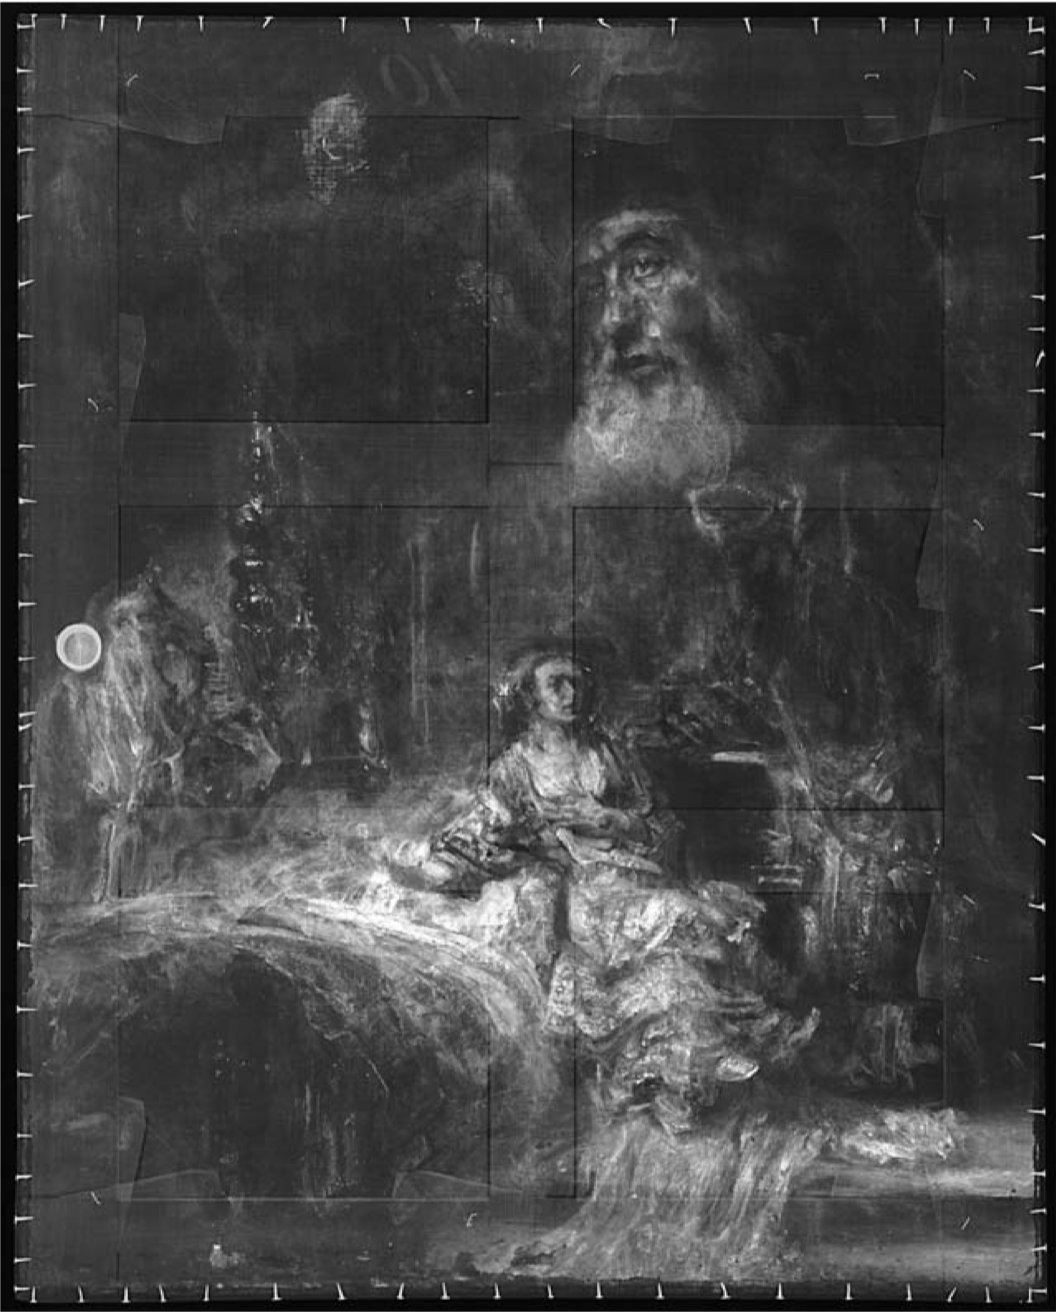
\includegraphics[width=0.5\textwidth]{img/demonstrationsmodell.png} \hfill}
    % ----------------------------------------------
    \column{0.5\textwidth}
    \begin{quote}
        So können etwa Veränderungen sichtbar gemacht
werden, die der Künstler während des Malens an einer
Komposition vorgenommen hat. Auch Manipulationen, die
von anderer Hand und zu einem späteren Zeitpunkt am
Original vorgenommen wurden, können auf diese Weise
„durchschaut“ werden.\\
{\scriptsize \href{https://web.archive.org/web/20140912212745/}{Link:} \href{http://www.arge-
kunstgeschichte.de/fileadmin/user\_upload/pdf/Der\_Blick\_durch\_die\_Bilder.pdf }{Der Blick durch die Bilder: Alte Meister geröntgt}, in: \protect\url{arge-kunstgeschichte.de}, S. 2.}
    \end{quote}

  \end{columns}
\end{frame}

%------------------------------------------------------------------------------

\begin{frame}[allowframebreaks]{Experimental models}
\metroset{block=fill}
\begin{quote}
„\punkti als Experimentalmodelle dienen sie der Ermittlung
oder Überprüfung von Hypothesen \punkti“~\parencite[139]{stachowiak}
\end{quote}
\begin{quote}
        Als Demonstrationsmodelle werden sie zur
Veranschaulichung von (weniger anschaulichen oder
unanschaulichen) Zusammenhängen benutzt, \punkti.~\parencite[138]{stachowiak}
\end{quote}\bigskip
    
    \begin{block}{Example}
    \begin{enumerate}\footnotesize
        \item \textbf{Hypothesis:} „The stronger the current, the lesser the pressure.“
        \item \textbf{Testing the hypothesis} using experiments
    \end{enumerate}
    \end{block}
    
    \framebreak
    
    \begin{columns}
    \column{0.45\textwidth}
    \begin{block}{}
        \href{https://youtu.be/K0aPuLn76H0}{Physics: Bernoulli effect}
    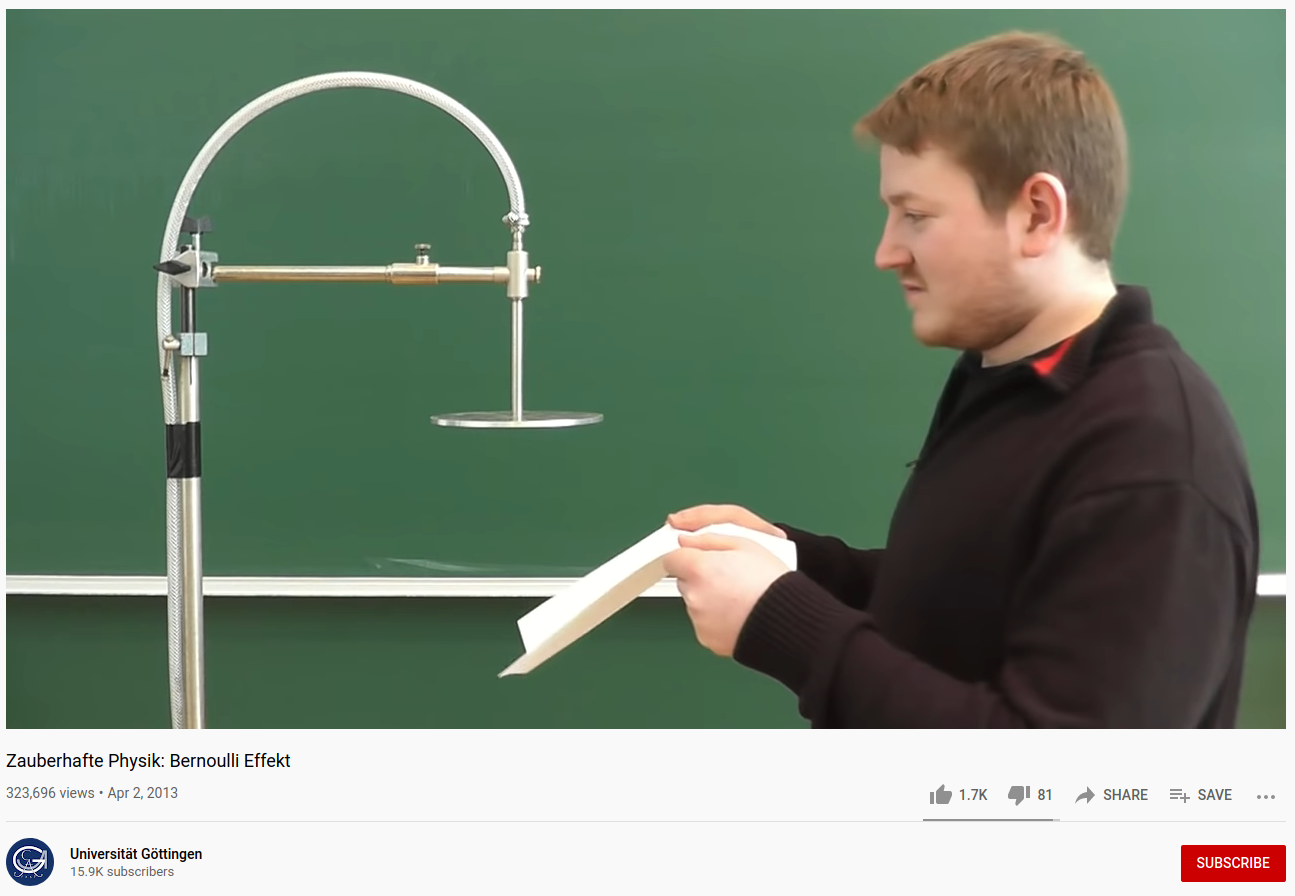
\includegraphics[width=\textwidth]{img/physik-bernoulli.png}
    \end{block}
    
    \column{0.45\textwidth}
    \begin{block}{}
        \href{https://www.youtube.com/watch?v=2vS4aPQI80M}{Recreating historical recipes}
    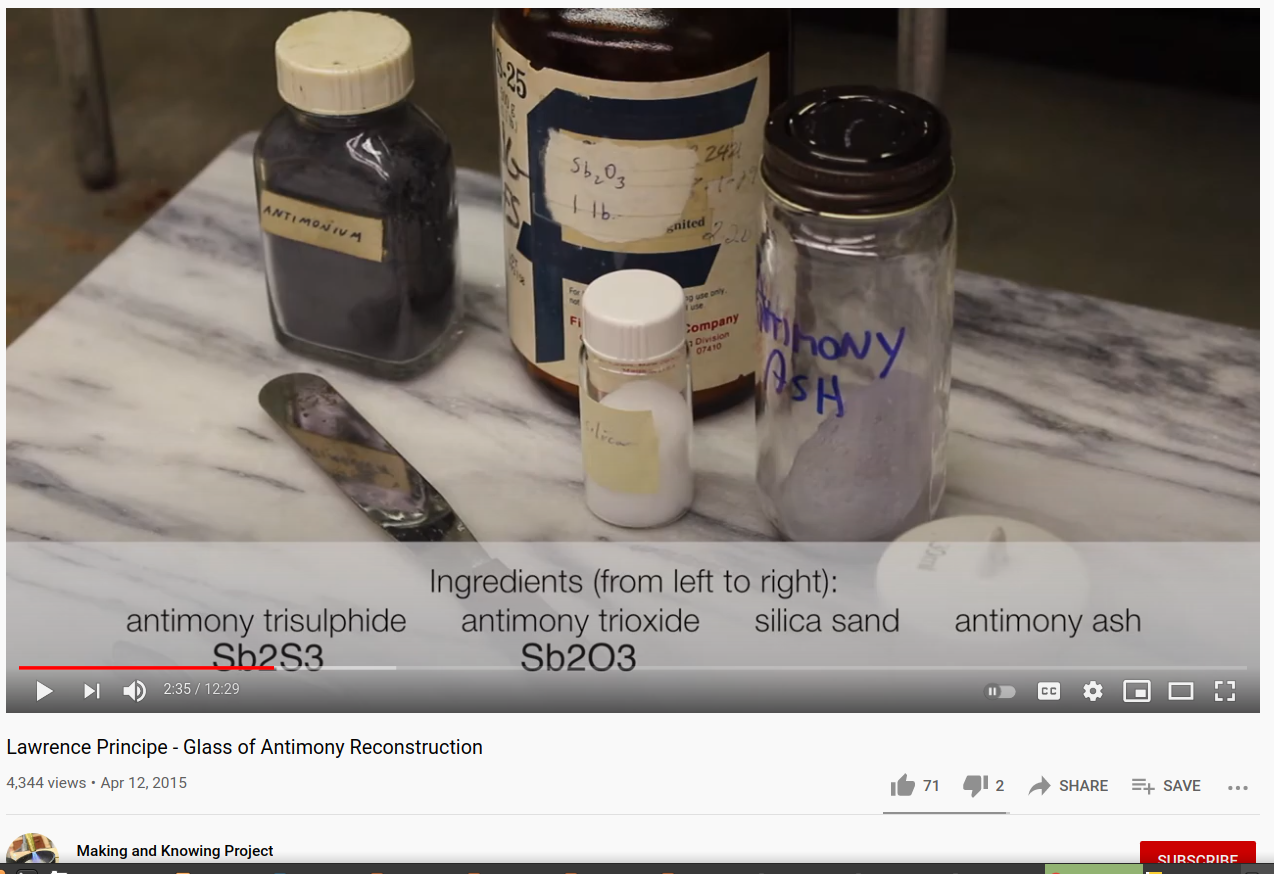
\includegraphics[width=\textwidth]{img/glass-of-antimony-experiment.png}
    
    \end{block}
    \end{columns}
    
\end{frame}

%------------------------------------------------------------------------------
\begin{frame}{Theoretical models}
  \begin{columns}%[T,onlytextwidth]
  \metroset{block=fill}
    \column{0.4\textwidth}
    \begin{block}{Stachowiak}
        \begin{quote}
            „\punkti als theoretische Modelle vermitteln sie in logisch bündiger Form Erkenntnisse über Sachverhalte,~\punkti“~\parencite[139]{stachowiak}.
        \end{quote}
    \end{block}

    % ----------------------------------------------
    \column{0.6\textwidth}
    \bigskip
    
    \begin{enumerate}
        \item \textbf{Rule:} All fish live in water.
        \item \textbf{Example:} Gold fish Hermann is a fish.
        \item \textbf{Result:} Hermann lives in water.
    \end{enumerate}
    \bigskip
    
    \begin{block}{Logic}
    $p \lor \neg p$
    \end{block}

  \end{columns}
\end{frame}

%------------------------------------------------------------------------------
\begin{frame}{Operative models}
  \begin{columns}%[T,onlytextwidth]
  \metroset{block=fill}
    \column{0.5\textwidth}
    \begin{quote} „Der wasserbauliche Modellversuch ist die beste
Methode, um Vorhersagen zu treffen, wie es in der
Natur aussieht, \punkti Die Ergebnisse der Untersuchungen sollen Aufschluss
darüber geben, ob das geplante Einlaufbauwerk
optimal dimensioniert ist und wann und wie die
Verschlüsse zu öffnen sind, um die gewünschte Wirkung
zu erzielen. \\
{\scriptsize \emph{Hochwasserschutz bei Kramsach im Modellversuch}, in: \protect\url{meinbezirk.at}. Stand: 04.02.2017.}
    \end{quote}
    % ----------------------------------------------
    \column{0.5\textwidth}
    \metroset{block=fill}
        \begin{block}{Stachowiak}
        \begin{quote}
            „\punkti und als operative Modelle möglicher Zielaußenwelten stellen sie ihren Benutzern Entscheidungs- und Planungshilfen zur Verfügung.“~\parencite[139]{stachowiak}
        \end{quote}
    \end{block}
    \metroset{block=fill}
      \begin{block}{}
      \href{https://www.youtube.com/watch?v=TbtdXpJvZiA\&t=78s}{Hochwasserschutz Radfeld}
      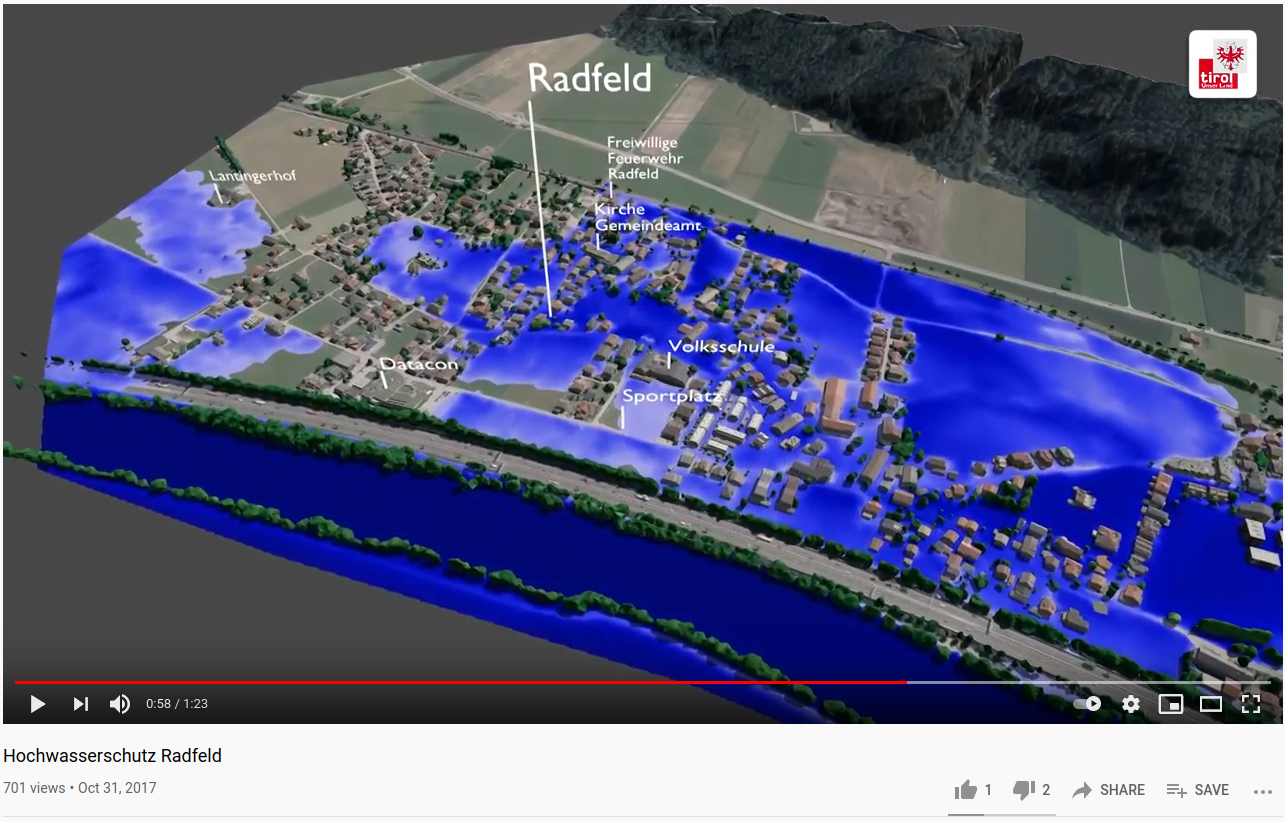
\includegraphics[width=0.95\textwidth]{img/radfeld-hochwasserschutz.png}
      \end{block}

  \end{columns}
\end{frame}

%------------------------------------------------------------------------------


%\begin{frame}[standout]    Homework and lecture\end{frame}
\subsection{Homework \& readings}

\begin{frame}{Homework: globe model}
\begin{itemize}
    \item the globe is a physical model of the world
    \item digital model = \href{https://www.google.at/maps/}{Google Maps}
    \begin{itemize}
        \item go on “Satellite“, zoom out.
        \item \href{https://earth.google.com}{Google Earth}
    \end{itemize}
    \item Which information or (abstract) knowledge is represented in those two models of the world?
    \item For which reasons or for what purpose can models (globe, Google Maps/Earth) be used to represent their original (the world)?
\end{itemize}

\metroset{block=fill}
\begin{alertblock}{Homework} \footnotesize
Take a globe or Google Maps/Earth, read chapters 2.1.3 of „Herbert Stachowiak: Allgemeine Modelltheorie“ (pdfs in the zip under "LEKTUERE", or in EN). If you can read it in German, please do so. 

Try to integrate what you have learned from reading Stachowiak.
Upload your solution (max. 1/2--1 page of text) to Moodle within the time period indicated.
The text should be readable, not bullet points. 
\end{alertblock}
\end{frame}

%------------------------------------------------------------------------------
\begin{frame}[standout]
    \alert{Reading} for next week: \\
    Stachowiak, all texts/PDFs (Nr. 02--04) \\
    \small (ca. 10 pages) 
\end{frame}
\section{General modelling theory II}
%------------------------------------------------------------------------------
\begin{frame}{Homework assignment solution: What knowledge is in a globe?}
\begin{columns}[T,onlytextwidth]
\column{0.45\textwidth}
\metroset{block=fill}
\begin{exampleblock}{\footnotesize What information or (abstract) knowledge is embodied or encoded in a globe or Google Maps/Earth? }
    \begin{itemize}\footnotesize
        \item form, rotation, tilt
        \item sizes, distances, topography: continents, bodies of water, mountains, vegetation 
        \item Borders and names of: states, cities, streets, \dots
        \item Places of Interest = POI (shops, traffic, tourism)
        \item Further information: population, traffic data, time zones
    \end{itemize}
\end{exampleblock}
% Aus welchen Gründen bzw. zu welchem Zweck könnten die Modelle zur Originalrepräsentation herangezogen werden?

\column{0.5\textwidth}
\begin{alertblock}{What can it be used for?}
\begin{enumerate}\small
    \item Navigation: plan your travel route
    \item capture borders, distances and locations
    \item explore the earth and its regions, places, etc.
\end{enumerate}
\end{alertblock}

\begin{alertblock}{How? (operating with the model)}
\begin{enumerate}\small
    \item directions / route planning form
    \item turning
    \item zooming in and out
    \item checking or removing certain layers
\end{enumerate}
\end{alertblock}
\end{columns}
\end{frame}

%------------------------------------------------------------------------------
\begin{frame}[allowframebreaks]{3 proporties of a model following Stachowiak}

\metroset{block=fill}
\begin{alertblock}{1)~ Mapping }
\begin{quote} \scriptsize
    „Modelle sind stets Modelle von etwas, nämlich Abbildungen, Repräsentationen natürlicher oder künstlicher Originale, die selbst wieder Modelle sein können.“ 
    %„Originale und Modelle werden hier ausschließlich als Attributklassen gedeutet, die oft die spezielle Gestalt attributiver Systeme erlangen.“ % 131
    „Der Abbildungsbegriff fällt mit dem Begriff der Zuordnung von Modell-Attributen zu Original-Attributen zusammen.“ \parencite[131--132]{stachowiak} % 132
    
    \alert{Models are always models of something, i.e. mappings from, representations of natural or artificial originals, that can be models themselves.}
\end{quote}
\end{alertblock}
\begin{alertblock}{2)~ Reduction}
\begin{quote} \scriptsize
    „Modelle erfassen im allgemeinen nicht alle Attribute des durch sie repräsentierten Originals, sondern nur solche, die den jeweiligen Modellerschaffern und/oder Modelbenutzern relevant scheinen.“ \parencite[132]{stachowiak}
    
    \alert{Models in general capture not all attributes of the original represented by them, but rather only those seeming relevant to their model creators and/ or model users.}
\end{quote}
\end{alertblock}
\framebreak 

\begin{alertblock}{3)~ Pragmatism}
\begin{quote} \scriptsize
    „Eine pragmatisch vollständige Bestimmung des Modellbegriffs hat nicht nur die Frage zu berücksichtigen, \emph{wovon} etwas Modell ist \lbrack{}Abbildungsmerkmal\rbrack{}, sondern auch, \emph{für wen, wann} und \emph{wozu} bezüglich seiner je spezifischen Funktionen es Modell ist.“ \parencite[132]{stachowiak} % 132
    
    \alert{ Models are not uniquely assigned to their originals per se. They fulfill their replacement function \\
    a) for particular – cognitive and/ or acting, model using subjects, \\
    b) within particular time intervals and \\
    c) restricted to particular mental or actual operations.}
\end{quote}
\end{alertblock}

\end{frame}


%------------------------------------------------------------------------------
\begin{frame}{Mapping using attributes}
  \begin{columns}[T,onlytextwidth]
  \metroset{block=fill}
    \column{0.45\textwidth}
    \begin{exampleblock}{\small Attributes versus predicates}
    \begin{quote}  \scriptsize
    %„Originale und Modelle werden hier ausschließlich als Attributklassen gedeutet, die oft die spezielle Gestalt attributiver Systeme erlangen.“ \parencite[131]{stachowiak}
    „\punkti alle Attribute \lbrack{}sind\rbrack{} als primär perzeptiv-kogitative Gebilde wohlzuunterscheiden von ihren sprachlichen -- gesprochenen oder geschriebenen oder sonstwie symbolisierten -- \emph{Artikulationen}.“ \parencite[135]{stachowiak}\smallskip
    
    „Es sei angenommen, daß es zu jeder Attributklasse wenigstens \emph{eine} sie elementweise repräsentierende Prädikatklasse gibt.“ \parencite[137]{stachowiak}
    
    \alert{$\to$ each attribute of the original has a predicate class in the model representing it.}
    \end{quote}
    \end{exampleblock}

    % ----------------------------------------------
    \column{0.5\textwidth}
    \metroset{block=fill}
    \begin{exampleblock}{Attributes = properties}
    \begin{quote}  \scriptsize
    %„Originale und Modelle werden hier ausschließlich als Attributklassen gedeutet, die oft die spezielle Gestalt attributiver Systeme erlangen.“ \parencite[131]{stachowiak}
    „Unter Attributen sind Merkmale und Eigenschaften von Individuen, Relationen zwischen Individuen, Eigenschaften von Eigenschaften, Eigenschaften von Relationen usw. zu verstehen.“ 
    „Hiernach sind einem beliebigen Original stets wohlunterscheidbare, nicht weiter zu zerlegende Teilobjekte zuzusprechen, die potentielle oder tatsächliche Träger von Eigenschaften sind und denen gegebenenfalls eine Relationenstruktur aufgeprägt werden kann.“ \parencite[134]{stachowiak}
    
    \alert{$\to$ properties should ideally be atomic}
    \end{quote}
    \end{exampleblock}
  \end{columns}
  \metroset{block=fill}
    \begin{block}{Mapping = assigning attributes between modell and original}
        \begin{quote}\scriptsize
            „Der Abbildungsbegriff fällt mit dem Begriff der Zuordnung von Modell-Attributen zu Original-Attributen zusammen.“ \parencite[132]{stachowiak}
        \end{quote}
    \end{block}
\end{frame}

%------------------------------------------------------------------------------
\begin{frame}{Mapping in the globe modell}
  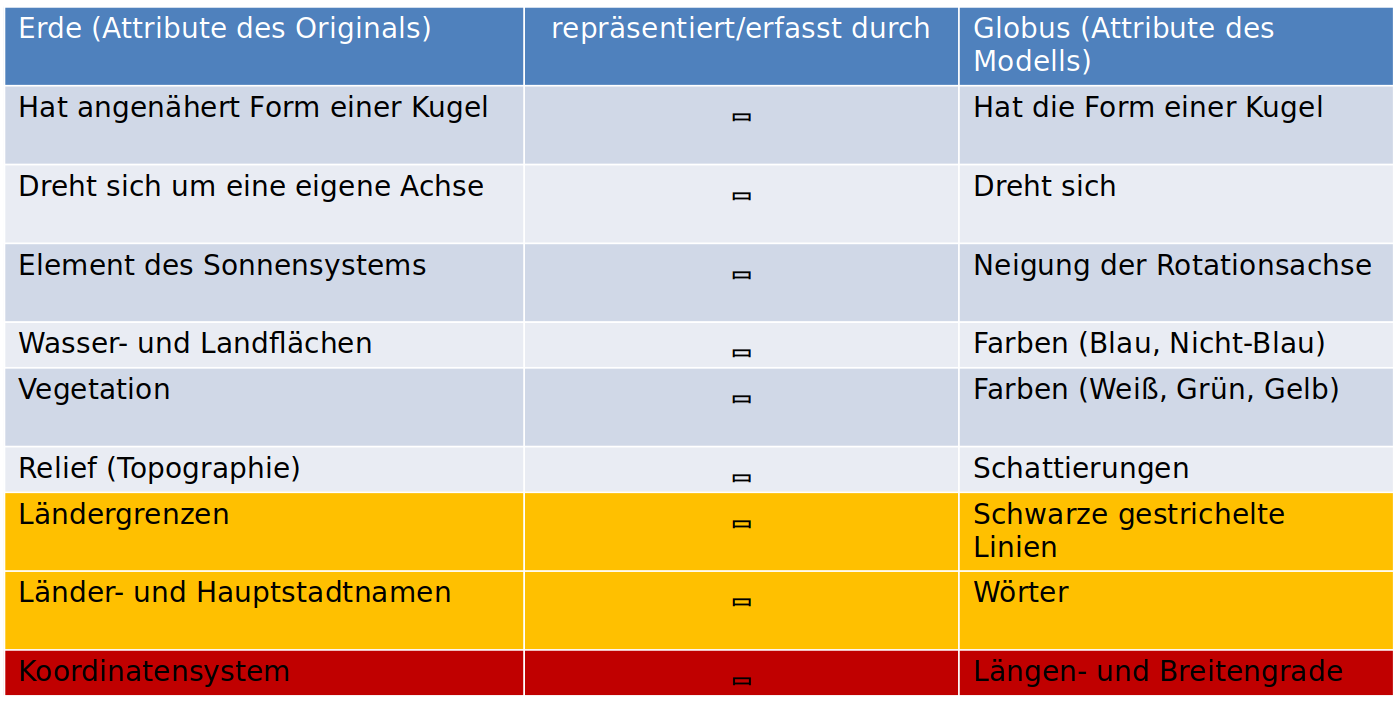
\includegraphics[width=\textwidth]{img/modell-globus.png}  
\end{frame}


%------------------------------------------------------------------------------
\begin{frame}[standout]
    \alert{Discussion:} \small \\  Which originals would you like to model? \\
    Which attributes of the original are to be represented? \\
    What reasons are there for that model?
\end{frame}


%------------------------------------------------------------------------------
\begin{frame}[standout]
    \alert{Reading} for next week: \\
    McCarty, Modelling 
\end{frame}



\section{Data modelling}


%------------------------------------------------------------------------------
\begin{frame}[allowframebreaks]{Data Modelling: Stachowiak's \emph{General Model Theory}}
\small 

\bg{alert}{white}{His notion of a model}
„Alle Erkenntnis ist Erkenntnis in Modellen oder durch Modelle und jede
menschliche Weltbegegnung überhaupt bedarf des Mediums Modell“ (Herbert Stachowiak 1973)
\alert{$\to$ All knowledge-making is knowledge-making in or through models and all human perception of the world needs models as a medium. }
\smallskip


\bg{alert}{white}{Data modelling}
Model = snippet of the real world but it only covers the attributes I chose to be relevant for the task at hand. 
Thus, the model and the aspect of the real world it models (its subject) diverge. 

\smallskip

\bg{alert}{white}{Model = abstraction (=class)}
concrete applications of the model (i.e. one concrete cooking recipe, poem, etc.) are called \emph{instances}.

\smallskip

Standardized models allow us to exchange and analyse data, search/query data. 
 $\to$ only \bg{alert}{white}{formal models} can be processed digitally, i.e. every digital model is a formal model.
\smallskip

\framebreak\small

\bg{alert}{white}{1) Mapping}
 {Models are always models of something, i.e. mappings from, representations of natural or artificial originals, that can be models themselves.}
\smallskip

\bg{alert}{white}{2) Reduction}
Models in general capture not all attributes of the original represented by them, but rather only those seeming relevant to their model creators and/ or model users. For example, I can only photograph (or even see!) a statue from one perspective at a time. I never see `the thing itself' but a partial aspect of all its defining properties. 

\smallskip

\bg{alert}{white}{3) Pragmatism}
 Models are not uniquely assigned to their originals per se. They fulfill their replacement function \\
 \footnotesize
    a) for particular – cognitive and/ or acting, model using subjects, \\
    b) within particular time intervals and \\
    c) restricted to particular mental or actual operations.

\smallskip


%\bg{alert}{white}{Modelle = vereinfachte Repräsentationen von Teilen der realen Welt.}

\end{frame}

%------------------------------------------------------------------------------
\begin{frame}[allowframebreaks]{McCarty}

\bg{alert}{white}{Willard McCarty, „Modeling: A Study in words and Meanings“ (2004)}
\begin{enumerate}
    \item A model is a representation of something, for example for research purposes.
    \item Modelling = hermeneutic process by which models are created and used to solve problems.
    \item \emph{model of} (descriptive) vs. \emph{model for} (i.e. architectural plan for building a house).
    \item modelling as an experimental process with the goal of capturing aspects of reality
\end{enumerate}
\framebreak

\bg{w3schools}{white}{Modelling as an interative process} \\
\begin{itemize}
    \item include present knowledge
    \item create model
    \item use for model to research the subject
    \item learn from discrepancies between model and real world to refine your model. 
    \item re-make the model to integrate new insights
    \item repeat
\end{itemize}

\end{frame}

%------------------------------------------------------------------------------
\begin{frame}[allowframebreaks]{Models = simplified repres. of parts of the real world }
\bg{w3schools}{white}{Model = mapping = representation $\neq$ original}: just parts of the original are represented. Choosing which parts depends on the intended use by which you later measure how useful (i.e. good) the model is. Or is the best model the most accurate? 

\bg{w3schools}{white}{subjective \& abstracted} $\to$ the model has to be created with reference to a specific research question and will only be useful (or the most useful) with regard to this question. Perception and representation are always selective \& subjective. Thus, so are the models. I can never capture all aspects at the same time. A photo of a vase only shows it from one side. 

\bg{w3schools}{white}{Metadata} can be used to enrich data models (supplying additional information, such as administrative or technical) 

\bg{w3schools}{white}{Disambiguation} $\to$ often necessary to represent something in the digital sphere (practical aspect of modelling), for example by using normalization, geonames, GND etc. $\to$ conventions so that we can be sure we are referring to the same thing on the internet.
\medskip

Where does the realistic `mapping' of reality end? At which point are we left with only a subjective perspective of reality ?

\framebreak

\bg{w3schools}{white}{What do we even mean by original?} The book whose materiality gets lost in the digital realm? The idea behind the book?
\smallskip

\bg{alert}{white}{Example Photogrammetry / Structure from Motion}

 (= creating 3D models from overlapping photos): \\
 \textbf{reality} $\to$ more info than on the images. \\
 \textbf{3D model:} you need 8 Pixels (the same pixel on 8 different images) for one point in the model $\to$ less information than the sum of the (at least 50) images used to create the model from. 
\end{frame}
%------------------------------------------------------------------------------

%------------------------------------------------------------------------------
\begin{frame}[standout]
    \alert{Readings} -- summary: \\
    McCarty, Modelling \\[1em]
    {\footnotesize Please \alert{\href{https://docs.google.com/presentation/d/1YrEMpuguN12pY02jj_RKidxV9G88WTt5cCtUQldCe8w/edit?usp=sharing}{create a 1 slide summary for your part per group}}; designate 1 person to present to the group. \\
    }
\end{frame}





%------------------------------------------------------------------------------
\begin{frame}[allowframebreaks]{ER erweitert}
    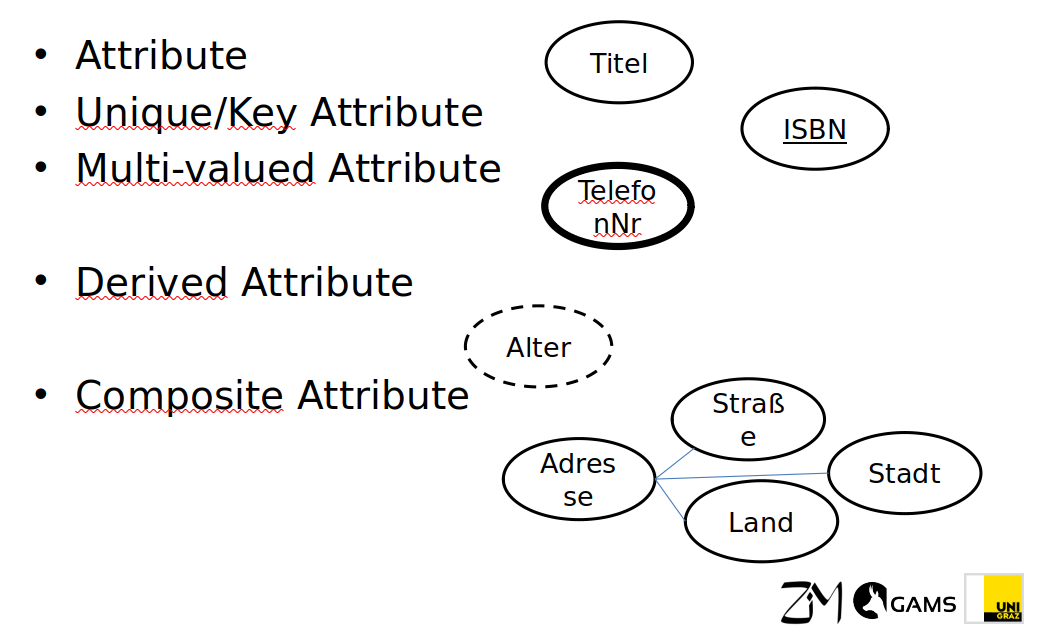
\includegraphics[width=\textwidth]{img/wdh-er-bestandteile.png}
    
    \framebreak
\footnotesize
\begin{tikzpicture}[node distance=6em]
\node[entity](book){book};
\node[attribute](isbn)[left of=book]{\key{ID}} edge(book);
\node[attribute](name)[above left of=book]{Name} edge(book);
\node[multi attribute](phone)[above of=book]{Phone} edge(book);
\node[attribute](address)[above right of=book]{Address} edge(book);
\node[attribute](street)[above right of=address]{Street} edge(address);
\node[attribute](city)[right of=address]{City} edge(address);
\node[derived attribute](age)[right of=book]{Age} edge(book);
\node[relationship](published)[below of=book]{published} edge(book);
\node[entity](tool)[below of=published]{Tool} edge[total](published);
\node[attribute](tid)[left of=tool]{\key{ID}} edge(tool);
\node[attribute](tname)[right of=tool]{Name} edge(tool);
\end{tikzpicture}

\footnotesize
\begin{tikzpicture}[node distance=6.5em]
%--------------------
% the book
%--------------------
\node[entity](book){Book};
\node[attribute](isbn)[left of=book]{\key{ISBN}} edge(book);
\node[attribute](title)[above left of=book]{title} edge(book);
\node[attribute](pagenr)[above of=book]{nr. of pages} edge(book);

%--------------------
% published by publisher
%--------------------
\node[relationship](published)[below of=book, yshift =-2em]{published} edge node[above right]{N}(book);
\node[entity](publisher)[below of=published, yshift =-2em]{publisher} edge node[above right]{1}(published);
\node[attribute](tid)[left of=publisher]{\key{ID}} edge(publisher);
\node[attribute](tname)[right of=publisher]{Name} edge(publisher);
\node[attribute](address)[above right of=publisher]{address} edge(publisher);
\node[attribute](street)[above right of=address]{Street} edge(address);
\node[attribute](city)[right of=address]{City} edge(address);
\node[multi attribute](phonenr)[below right of=publisher]{phone number} edge(publisher);

%--------------------
% written by author
%--------------------
\node[relationship](written)[right of=  book, xshift =3em]{written} edge node[above right]{N}(book);
\node[entity](author)[right of= written, xshift =3em]{author} edge node[above right]{M}(written);
\node[attribute](birthday)[above  of=author]{birthday} edge(author);
\node[attribute](name)[above right of=author]{name} edge(author);
\node[derived attribute](age)[right of=author]{Age} edge(author);
\end{tikzpicture}


\end{frame}


%------------------------------------------------------------------------------
\section{Entity-Relationship Model (ERM)}
%------------------------------------------------------------------------------

%------------------------------------------------------------------------------
\begin{frame}{Das Entity-Relationship Model nach Peter Chen}
\metroset{block=fill}
\begin{block}{\cite[9]{chen1976}}
    \begin{quote}
        The entity-relationship model can be used as a basis for unification of different views of data: the network model, the relational model, and the entity set model.~
    \end{quote}
\end{block}
\begin{block}{\cite[10]{chen1976}}
    \begin{quote}
        \lbrack{}Der Text\rbrack{} analyzes the network model, the relational model, and the entity set model, and describes how they may be derived from the entity relationship model.~
    \end{quote}
\end{block}
\begin{block}{\cite[19]{chen1976}}
    \begin{quote}
        \lbrack{}Der Text stellt vor:\rbrack{} a diagrammatic technique for exhibiting entities and relationships: the entity-relationship diagram.~%\parencite[19]{chen1976}
    \end{quote}
\end{block}
$\to$ \alert{Konzeptuelles Modell}

\end{frame}

%------------------------------------------------------------------------------
\begin{frame}{ER-Begriffe~\parencite[9--12]{chen1976}}
    % ----------------------------------------------
  \begin{columns}[T,onlytextwidth]
  \metroset{block=fill}
    \column{0.55\textwidth}\footnotesize
      \begin{block}{Entität (Entity)}
       An entity is a „thing“ which can be distinctly identified. A specific person, company, or event is an example of en entity.
      \end{block}

      \begin{alertblock}{Beziehung (Relationship)}
        A relationship is an association among entites. For instance, „father-son“ is a relationship between two „person“ enitities.
      \end{alertblock}

      \begin{exampleblock}{Entitätsmenge (Entity Set)}
        Alle Entitäten derselben Entitätsmenge haben dieselben Eigenschaften (properties). 
        
        „Entities are classified into different entity sets such as EMPLOYEE, PROJECT, and DEPARTMENT.“
      \end{exampleblock}

    % ----------------------------------------------

    \column{0.4\textwidth}

      \metroset{block=fill}

      \begin{block}{ER-Modell-Bestandteile}
      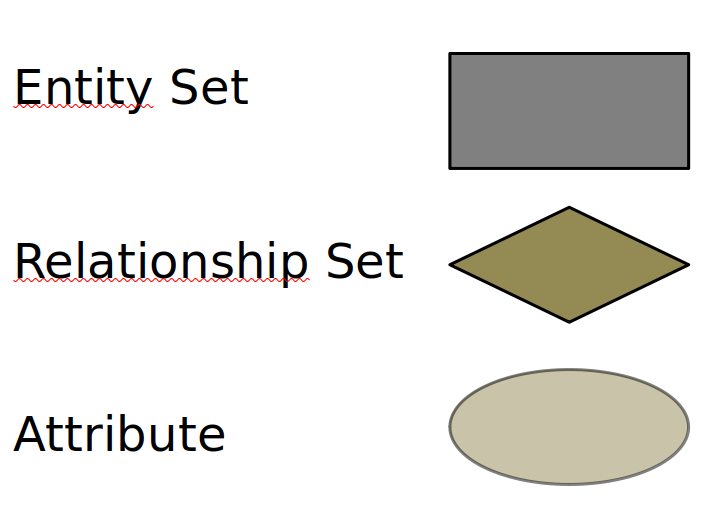
\includegraphics[width=0.9\textwidth]{img/er-modell.png}
      \end{block}
      
      \begin{block}{ER-Modell-Bestandteile}
      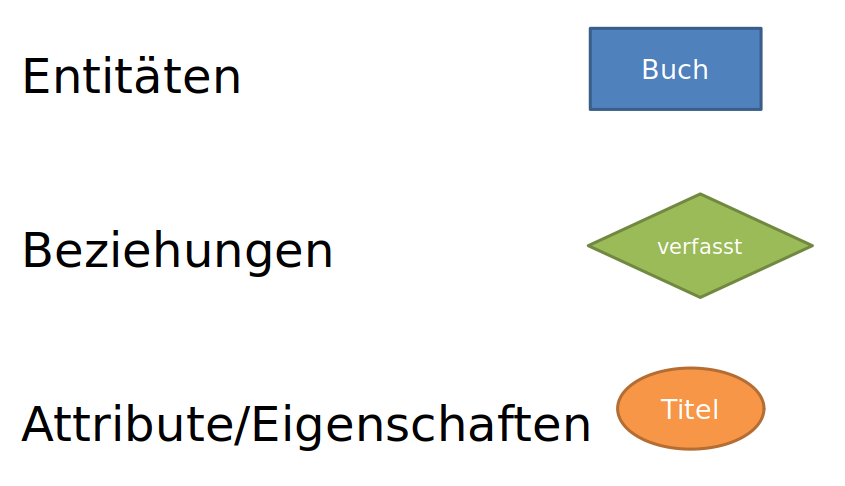
\includegraphics[width=0.9\textwidth]{img/er-bsp2.png}
      \end{block}
  \end{columns}

\end{frame}

%------------------------------------------------------------------------------
\begin{frame}{ER-Begriffe~\parencite[9--12]{chen1976}}
    % ----------------------------------------------
  \begin{columns}[T,onlytextwidth]
  \metroset{block=fill}
    \column{0.48\textwidth}\footnotesize
      \begin{exampleblock}{Menge von Beziehungen (Relationship Set)}
        Gleiche Beziehungen zwischen Entitäten, die jeweils aus derselben Entitätsmenge stammen, lassen sich in einer Menge von Beziehungen zusammenfassen. 
      \end{exampleblock}

    % ----------------------------------------------

    \column{0.48\textwidth}

      \metroset{block=fill}
      \begin{block}{Rolle (Role)} \footnotesize
        The role of an entity in a relationship is the function that it performs in the relationship.
      \end{block}
      
      \begin{alertblock}{Eigenschaften (Properties)}\footnotesize
        Mithilfe von Eigenschaften lassen sich Entitäten (Entities) und Beziehungen (Relationships) beschreiben. 
      \end{alertblock}
  \end{columns}
  \begin{center}
      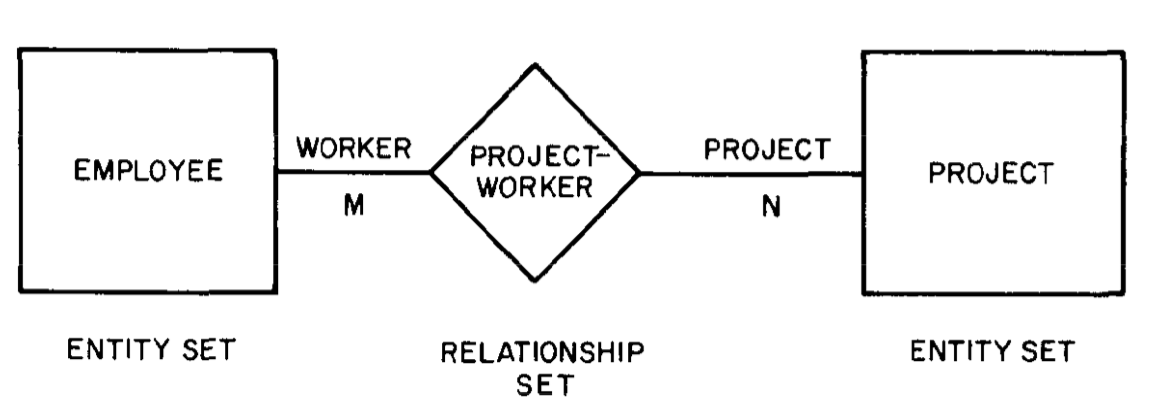
\includegraphics[width=0.6\textwidth]{img/er-bsp.png}
  \end{center}
\end{frame}

%------------------------------------------------------------------------------
\begin{frame}{Attribut-Wert-Paare und Primary Keys}
    Eigenschaften (Properties) werden stets durch eine Kombination von Attribut und Wert ausgedrückt. Beispiel: 
    \begin{enumerate}
        \item Der Stift ist blau = Die Entität `Stift' hat das Attribut „Farbe“ mit dem Attributwert „blau“ 
        \item Der Stift ist rot = Die Entität `Stift' hat das Attribut „Farbe“ mit dem Attributwert „rot“
    \end{enumerate}

\metroset{block=fill}
\begin{exampleblock}{Primary Key: Identifizierende Eigenschaften}
Entitäten und Beziehungen lassen sich über den Wert eines oder mehrerer Attribute identifizieren. 
Das oder die identifizierenden Attribute werden als Primary Key bezeichnet.
\end{exampleblock}
\end{frame}
%------------------------------------------------------------------------------
\begin{frame}[allowframebreaks,fragile]{Beispiel ER-Modell für ein Buch}
\begin{comment}
    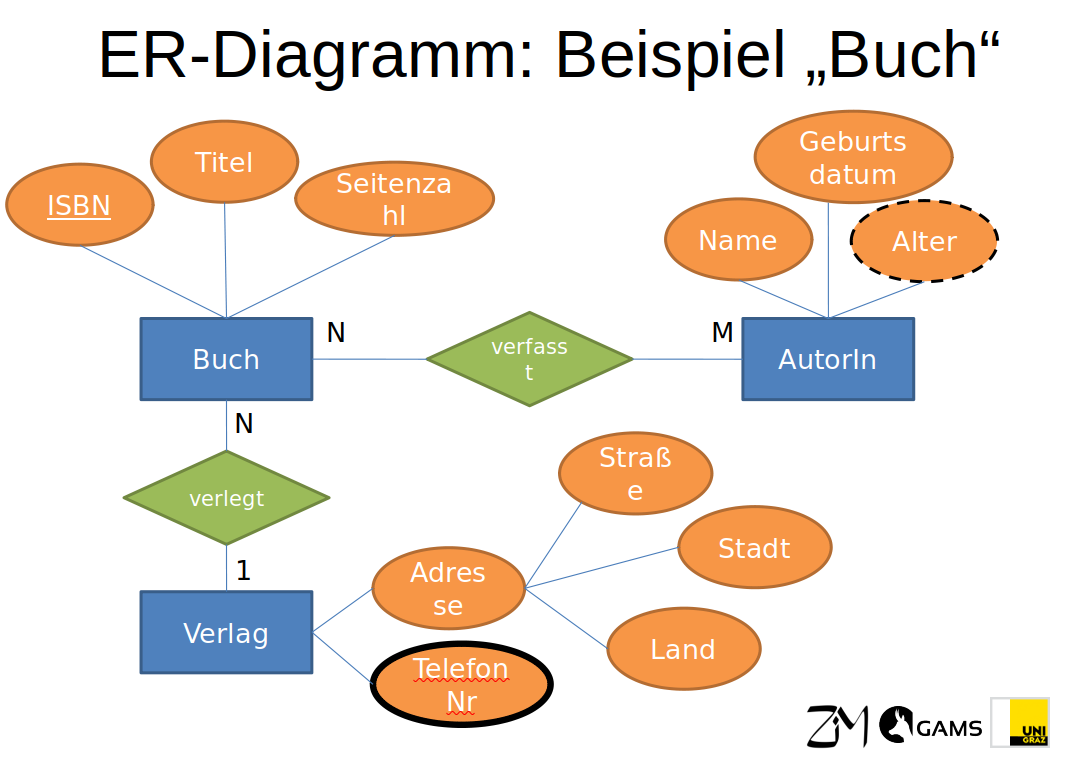
\includegraphics[width=0.9\textwidth]{img/er-bsp3.png} 
    
    \framebreak
\end{comment}

\footnotesize
\begin{tikzpicture}[node distance=5.5em]
%--------------------
% the book
%--------------------
\node[entity](book){Book};
\node[attribute](isbn)[left of=book]{\key{ISBN}} edge(book);
\node[attribute](title)[above left of=book]{title} edge(book);
\node[attribute](pagenr)[above of=book]{nr. of pages} edge(book);

%--------------------
% published by publisher
%--------------------
\node[relationship](published)[below of=book, yshift =-2em]{published} edge node[above right]{N}(book);
\node[entity](publisher)[below of=published, yshift =-2em]{publisher} edge node[above right]{1}(published);
\node[attribute](tid)[left of=publisher]{\key{ID}} edge(publisher);
\node[attribute](tname)[right of=publisher]{Name} edge(publisher);
\node[attribute](address)[above right of=publisher]{address} edge(publisher);
\node[attribute](street)[above right of=address]{Street} edge(address);
\node[attribute](city)[right of=address]{City} edge(address);
\node[multi attribute](phonenr)[below right of=publisher]{phone number} edge(publisher);

%--------------------
% written by author
%--------------------
\node[relationship](written)[right of=  book, xshift =3em]{written} edge node[above right]{N}(book);
\node[entity](author)[right of= written, xshift =3em]{author} edge node[above right]{M}(written);
\node[attribute](birthday)[above  of=author]{birthday} edge(author);
\node[attribute](name)[above right of=author]{name} edge(author);
\node[derived attribute](age)[right of=author]{Age} edge(author);
\end{tikzpicture}

\end{frame}


%------------------------------------------------------------------------------
\begin{frame}[fragile]{Beispiele}
\metroset{block=fill}
\begin{block}{Entitäten: Unikurs}
    \begin{itemize}
        \item \textbf{Entitäten:} Kurs, Dozent:in, Studierende, Raum
        \item \textbf{Attribute:} Kurs (Nr, Titel), Dozent:in (Name), Studierende (Name, Matrikelnummer, Studium, Fach), Raum (Nr, Gebäude, Sitzplätze)
        \item \textbf{Relationen:}
        \begin{itemize}
            \item Ein Kurs wird abgehalten von Dozent:in.
            \item Er findet in einem Raum statt.
            \item Die Studierenden nehmen am Kurs teil.
        \end{itemize}
    \end{itemize}
\end{block}

\begin{block}{CSV: Geburtsort}\scriptsize
\begin{verbatim}
    "Name","Address","Description","Longitude","Latitude"
    "Vorname Nachname","Teststr. 1, PLZ","Geburtsort","7.018242","50.678667"
\end{verbatim}
\end{block}
\end{frame}


%------------------------------------------------------------------------------
\begin{frame}[allowframebreaks]{(Materialien für die) Hausübung}
\metroset{block=fill}
\begin{exampleblock}{Ressourcen}
    \begin{itemize}\footnotesize
        \item \href{https://erdplus.com/standalone}{Tool zum Entity-Relationship-Modelle erstellen}
        \item \href{https://www.geeksforgeeks.org/introduction-of-er-model/}{GeeksforGeeks-Tutorial/Intro to ER Models}
        \item \href{https://geobrowser.de.dariah.eu/}{DARIAH Geobrowser}

    \end{itemize}
\end{exampleblock}

\begin{alertblock}{Angabe HÜ ER-Model}
    \begin{enumerate}\footnotesize
        \item Konzipieren und visualisieren Sie das Model Ihres Originals (Attributklasse) mithilfe des Entity-Relationship-Diagramms. (z.B. ERDplus siehe oben)
        \item Exportieren Sie ihr Diagramm als Bild und laden es auf Moodle hoch.
        \item Bei Problemen können Sie sich auch gegenseitig im Hilfe-Forum unterstützen.
        %\item Schauen Sie sich das Thema `Kardinalität' an bzw. erarbeiten es sich aus den Unterlagen und bauen Sie es in Ihr Modell ein. 
    \end{enumerate}
\end{alertblock}
\end{frame}

%------------------------------------------------------------------------------
%\begin{frame}[standout]
%    \alert{Lektüre} auf nächste Einheit: \\
%    Chen, ER-Modelle 
%\end{frame}

%\section{ER-Modelle (Wiederholung und Fortsetzung)}
\begin{frame}[allowframebreaks]{Kardinalitäten}
\metroset{block=fill}
    "Kardinalität" =  Anzahl der an einer Beziehung beteiligten Entitäten
    Dabei stehen \textit{n} und \textit{m} für eine beliebig hohe Anzahl.

\begin{block}{Typen von Relationen}
 \textbf{1:1} $\to$ Es gibt genau je eine Entität, die an der Beziehung beteiligt ist.
 
 \textbf{1:n} $\to$ Für jede Entität auf der 1-Seite der Beziehung kann es beliebig viele Entitäten auf der n-Seite geben.
 
 \textbf{n:m} $\to$ Für jede Entität auf der n-Seite der Beziehung kann es beliebig viel Entitäten auf der m-Seite geben und umgekehrt.
\end{block}

\begin{center}
  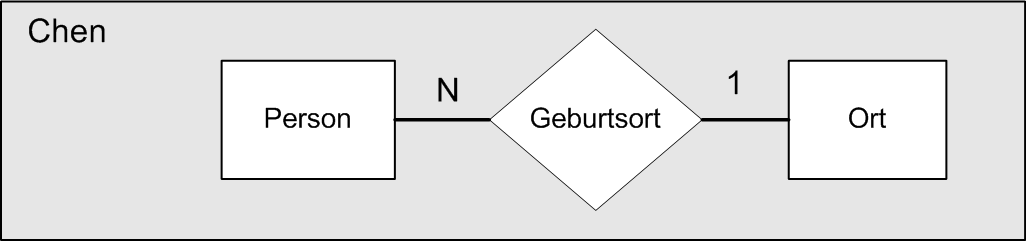
\includegraphics[width=0.7\textwidth]{img/ERD_Darstellungen_Chen.png}
\end{center}

\framebreak
\begin{block}{Minimale Kardinalitäten}
\textbf{0} $\to$ Es muß keine Entität auf dieser Seite der Beziehung geben. (=\textit{optional})

\textbf{1} $\to$ Es muß mindestens eine Entitäten auf dieser Seite der Beziehung geben. (=\textit{verpflichtend})
\end{block}

\begin{center}
    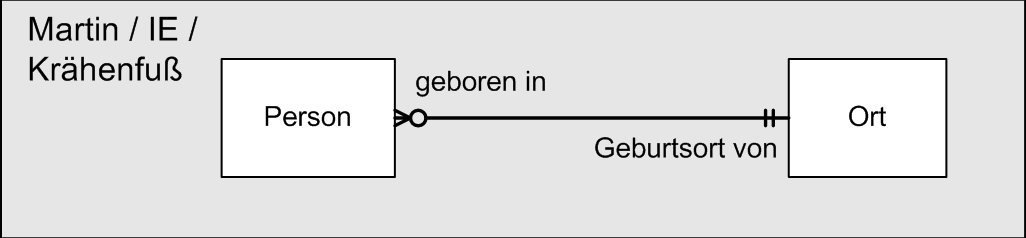
\includegraphics[width=0.7\textwidth]{img/ERD_Darstellungen_Crowfoot.png}
    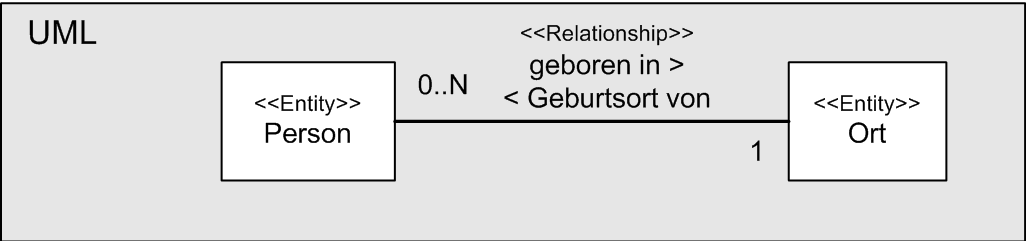
\includegraphics[width=0.7\textwidth]{img/ERD_Darstellungen_UML.png}
\end{center}

\end{frame}

%------------------------------------------------------------------------------
\begin {comment}
\begin{frame}{Wiederholung: ER-Begriffe~\parencite[9--12]{chen1976}}
    % ----------------------------------------------
  \begin{columns}[T,onlytextwidth]
  \metroset{block=fill}
    \column{0.55\textwidth}\footnotesize
      \begin{block}{Entität (Entity)}
       An entity is a „thing“ which can be distinctly identified. A specific person, company, or event is an example of en entity.
      \end{block}

      \begin{alertblock}{Beziehung (Relationship)}
        A relationship is an association among entites. For instance, „father-son“ is a relationship between two „person“ enitities.
      \end{alertblock}

      \begin{exampleblock}{Entitätsmenge (Entity Set)}
        Alle Entitäten derselben Entitätsmenge haben dieselben Eigenschaften (properties). 
        
        „Entities are classified into different entity sets such as EMPLOYEE, PROJECT, and DEPARTMENT.“
      \end{exampleblock}

    % ----------------------------------------------

    \column{0.4\textwidth}

      \metroset{block=fill}

      \begin{block}{ER-Modell-Bestandteile}
      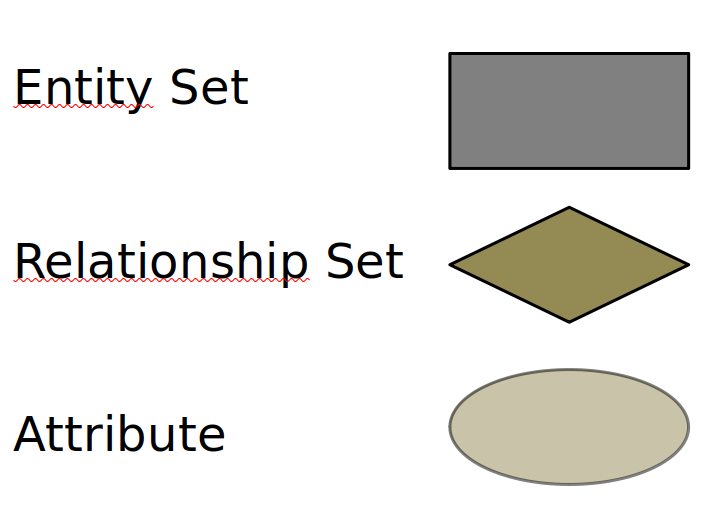
\includegraphics[width=0.9\textwidth]{img/er-modell.png}
      \end{block}
      
      \begin{block}{ER-Modell-Bestandteile}
      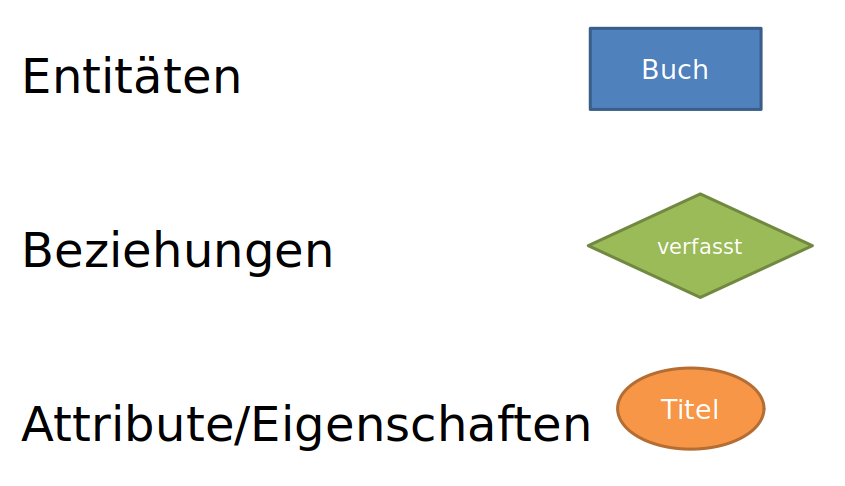
\includegraphics[width=0.9\textwidth]{img/er-bsp2.png}
      \end{block}
  \end{columns}

\end{frame}
\end{comment}

%------------------------------------------------------------------------------
\begin{frame}[allowframebreaks]{ER erweitert}
    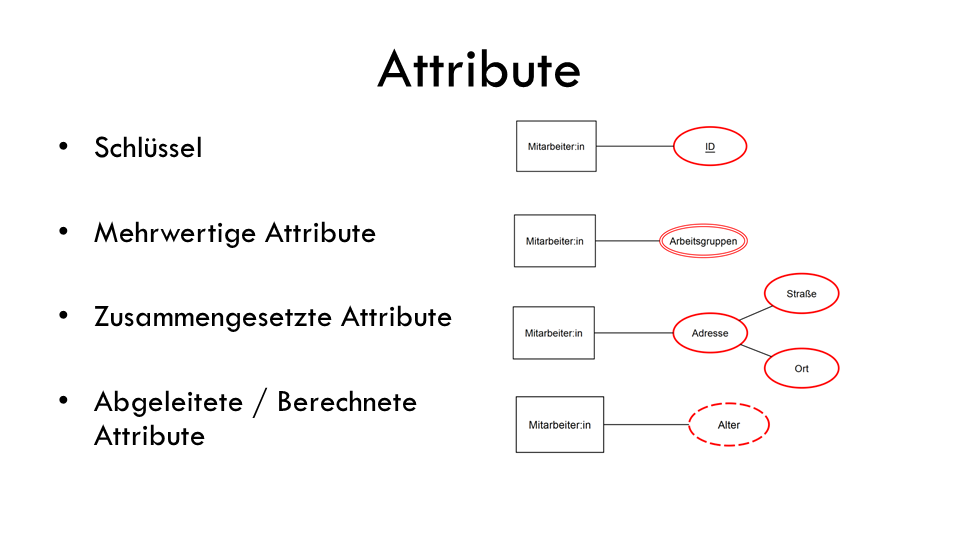
\includegraphics[width=\textwidth]{img/attribute.png}
\end{frame}



%\begin{comment}
\begin{frame}[allowframebreaks]{ER erweitert}
    \begin{itemize}
        \item \textbf{identifizierende Attribute (``Schlüssel``)}: Innerhalb der Entitätsklasse gibt es die Werte dieses Attributs nur genau einmal. Sie können damit die einzelne Entität identifizieren.
        \item \textbf{Mehrwertige Attribute}: Attribute, die mehr als einen Wert enthalten können.
        \item \textbf{abgeleitete Attribute}: Attribute, die sich aus einem anderen Attribut berechnen.
        \item \textbf{zusammengesetzte Attribute}: Attribute, die aus mehreren Teilen bestehen.
    \end{itemize}
    \begin{itemize}
        %\item \textbf{Attribute von Beziehungen}: Auch Beziehungen können Attribute haben.
        \item \textbf{n-äre Beziehungen}: ein Relationship-Set kann prinzipiell mehrere Entity-Sets mit einander verbinden.
        \item \textbf{Schwache Entität}: Kann nur existieren, wenn eine Relation zu einer anderen Entity existiert (Raum in Gebäude), Schlüssel ist abhängig vom Schlüssel einer Relationship (Chen-Notation: Doppelter Rand). Besitzen keine Eigenschaften, anhand derer man sie identifizieren könnte (besitzen keinen Primary Key). Sie werden nur über die Beziehung der schwachen Entität zu einer starken Entität identifiziert. Beispiel: der Angehörige eines Mitarbeiters eines Unternehmens
    \end{itemize}
\end{frame}
%\end{comment}

%-------------------------------------------------
    
\begin{frame}{n-äre Beziehungen}
\begin{center}
    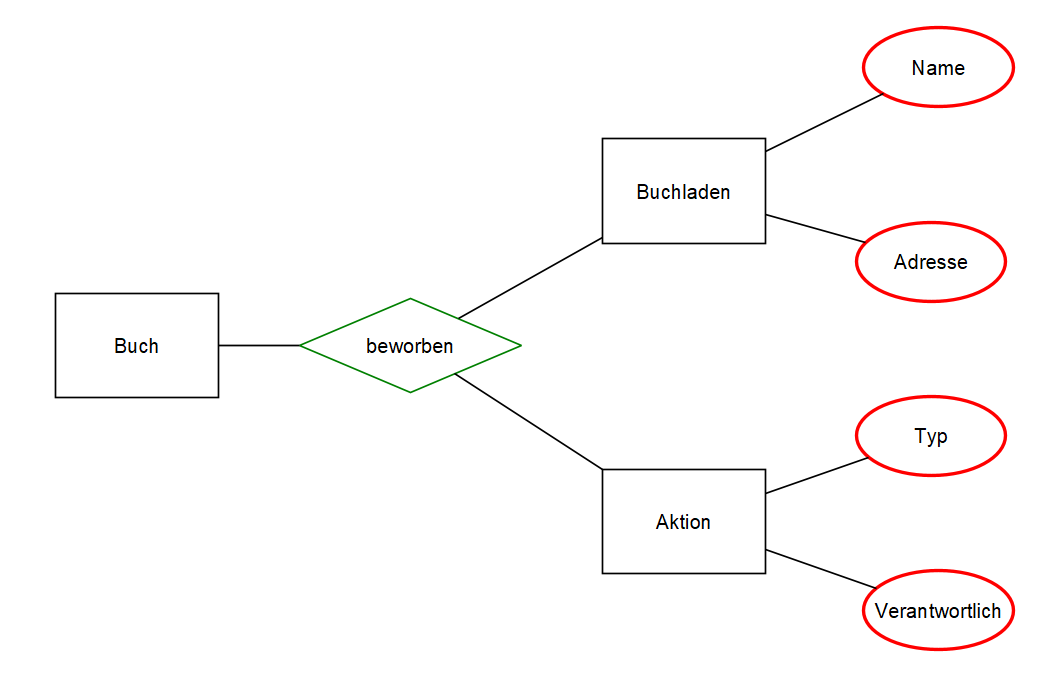
\includegraphics[width=0.9\textwidth]{img/n-ary-relationship.png}
\end{center}    
\end{frame}


%------------------------------------------------------------------------------
\begin{frame}{Übung ER-Modell}
    % ----------------------------------------------
  \begin{columns}%[T,onlytextwidth]
  \metroset{block=fill}
    \column{0.4\textwidth}\footnotesize
    \begin{block}{Eine Kurseinheit einer Lehrveranstaltung}
    Eine Kurseinheit besteht aus folgenden Enitäten:
    \begin{enumerate}
        \item Studierende
        \item Lehrende
        \item Sitzplatz
        \item Kursraum
        \item Gebäude
    \end{enumerate}
    \end{block}

    % ----------------------------------------------

    \column{0.55\textwidth}
      \metroset{block=fill}\footnotesize
      \begin{exampleblock}{Übung}
      \begin{enumerate}
          \item Mit welchen Attributen lassen sich diese Entitäten beschreiben?
          \item Anhand welcher Attribute lassen sich die Entitäten jeweils identifizieren?
          \item Welche Beziehungen existieren zwischen den Entitäten?
      \end{enumerate}
      $\to$ bezogen auf normalen Präsenzunterricht
      \end{exampleblock}
      \begin{exampleblock}{Übung 2}
      Wie müsste man das jetzt umändern, um auch Distance Learning einzukalkulieren?
      \end{exampleblock}
      \footnotesize
      $\to$ Übung in Gruppen. Erstellen Sie, wenn möglich, eine Zeichnung / einen Screenshot der Resultate, der dann vorgestellt wird.
  \end{columns}

\end{frame}


%------------------------------------------------------------------------------
\begin{frame}{Musterlösung Kurseinheit als ER}
    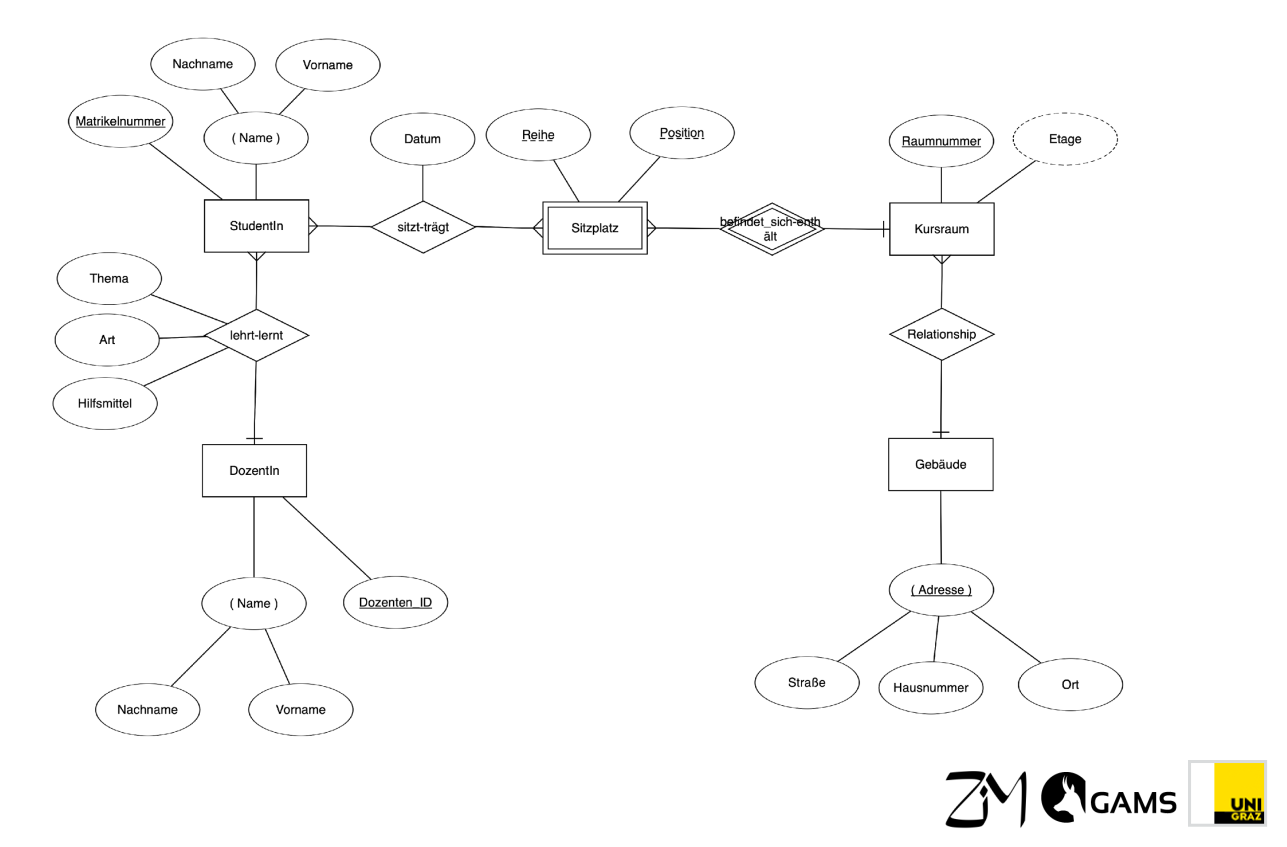
\includegraphics[width=\textwidth]{img/wdh-er-kursmodellierung.png}
\end{frame}


\subsection{ERM -- Tabellen und Relationen}
%------------------------------------------------------------------------------

%------------------------------------------------------------------------------
\begin{frame}{Von ER zur Tabelle?}
    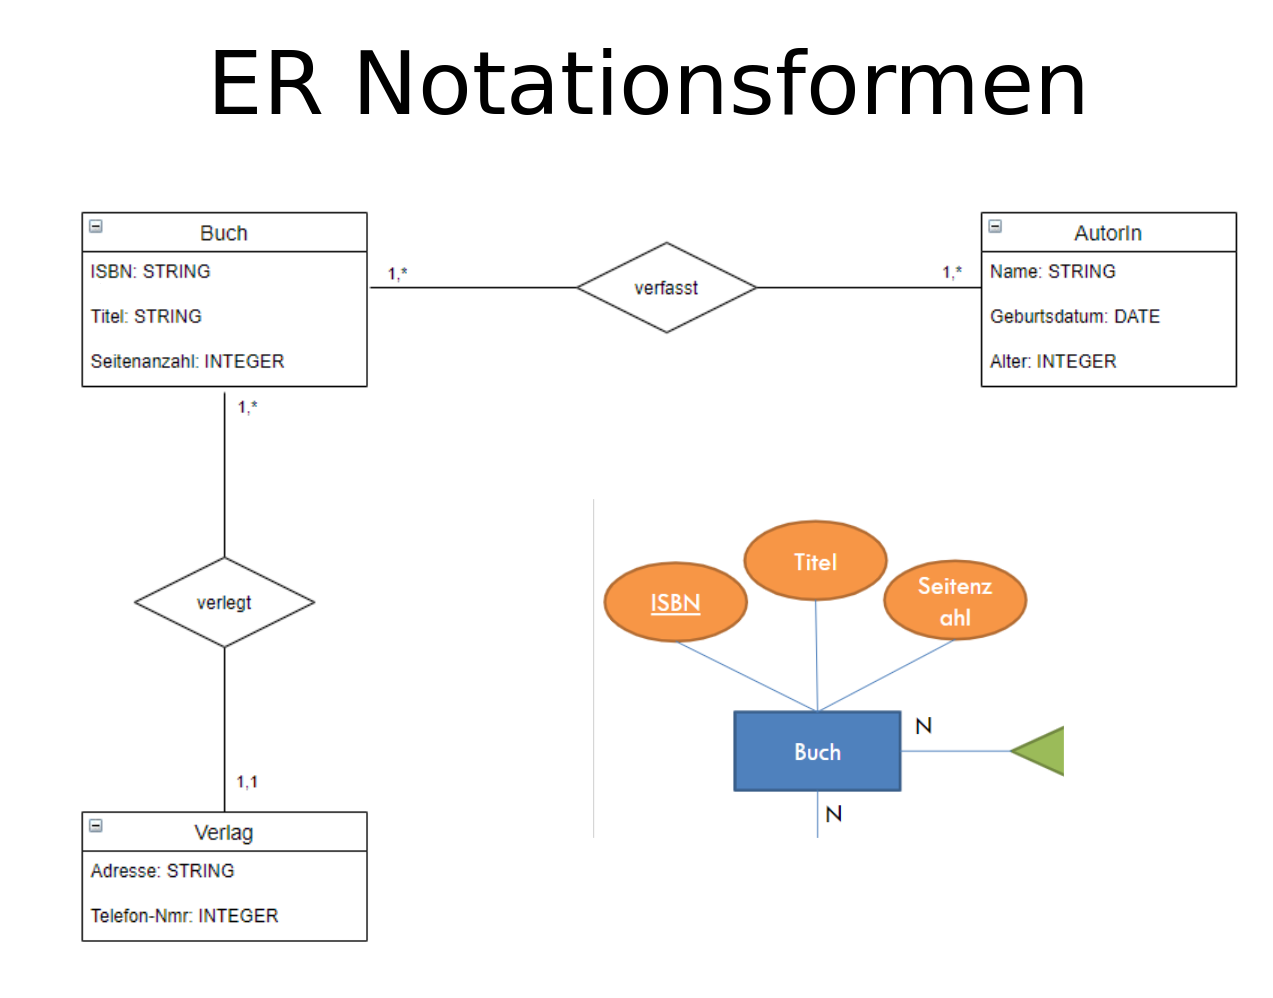
\includegraphics[width=\textwidth]{img/er-notation-buch.png}
\end{frame}

%------------------------------------------------------------------------------
\begin{frame}{Repräsentation von ER-Modellen als Tabellen}
    % ----------------------------------------------
  \begin{columns}[T,onlytextwidth]
  \metroset{block=fill}
    \column{0.4\textwidth}\footnotesize
    \begin{block}{Repräsentation als Tabellen}
    Entitäten und deren Beziehungen können als Tabellen repräsentiert werden. \\
    Die Attribute sind dann die Spalten
    \end{block}

    % ----------------------------------------------

    \column{0.55\textwidth}
      \metroset{block=fill}
      \begin{exampleblock}{Umgang mit Kardinalitäten}
      \begin{enumerate}\small
          \item Gleiches Buch aber mehrere Autoren? (Wieso nicht einfach als Attribut?)
          \item Gleiches Buch mehrere Genre? (Entität oder Attribut)
          \item Wie würde ich den Inhalt eines Buches modellieren?
      \end{enumerate} \small
      %$\to$ diese Leitfragen bitte in der Lektüre-Diskussion später auch beachten (beim Thema Kardinatlität)
      \end{exampleblock}

  \end{columns}
\end{frame}

%------------------------------------------------------------------------------
\begin{frame}{Entitäten und Attribute in Tabelle(n) überführen: Bsp. Kursmodellierung}
    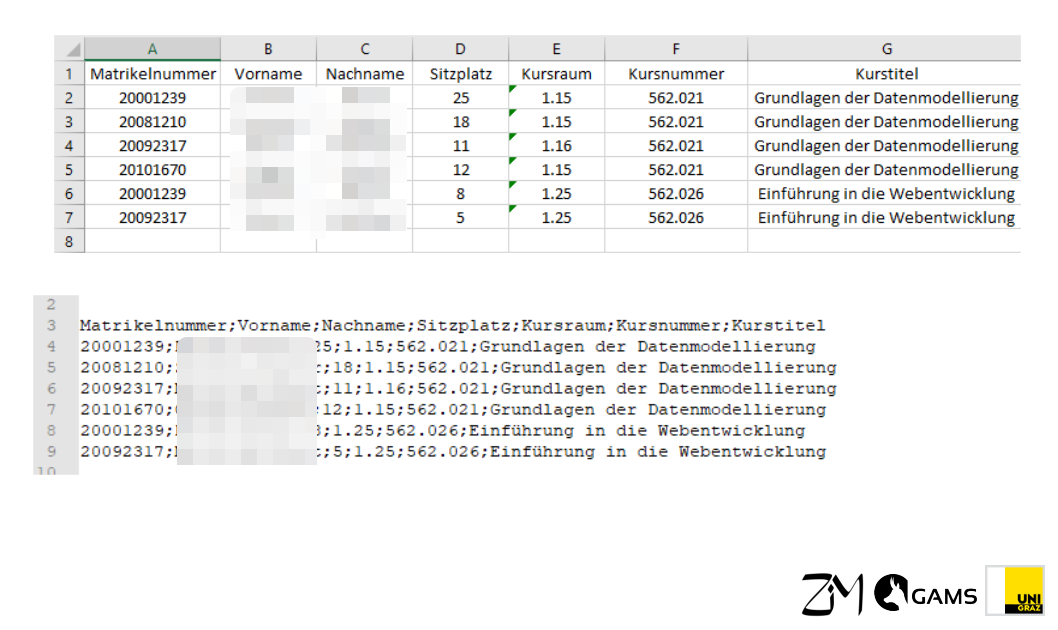
\includegraphics[width=\textwidth]{img/wdh-studierende-csv.png}
\end{frame}

%------------------------------------------------------------------------------
\begin{frame}[allowframebreaks]{Repräsentation von ER-Modellen als Tabellen}
    \begin{itemize}
        \item Entitätsklasse $\to$ Tabelle
        \item Attributklasse $\to$ Spalte
        \begin{itemize}
            \item mehrwertige Attribute $\to$ eigene Tabelle
        \end{itemize}
        \item Relation
            \begin{itemize}
                \item 1:1 $\to$ Schlüssel der einen Entität (Tabelle) wird als Referenz ("foreign key"/"Fremdschlüssel") in der anderen Tabelle eingefügt (eigene Spalte). 
                \item 1:n $\to$ Schlüssel der 1-seitigen Entität (Tabelle) wird als Referenz ("foreign key"/"Fremdschlüssel") in der n-seitigen Tabelle eingefügt (eigene Spalte)
                \item n:m $\to$ eigene Tabelle, die die Schlüssel der beiden Entitäten als Spalten enthält
                \item n-äre Relationen $\to$ eigene Tabelle, die die Schlüssel aller Entitäten als Spalten enthält
                \item Attribute zu Relationen $\to$ eigene Tabelle, die die Schlüssel der beteiligten Entitäten als Spalten und Spalten für die Attribute enthält
                \item mehrwertige Attribute $\to$ eigene Tabelle, die den Schlüssel der Entität als Fremdschlüssel enthält (also wie eine 1:n-Relation modelliert wird) und eine Spalte für das Attribut enthält.
                \item zusammengesetzte Attribute $\to$ eigene Tabelle, die den Schlüssel der Entität als Fremdschlüssel enthält (also wie eine 1:n-Relation modelliert wird) und Spalten für die  Teilattribute enthält.
            \end{itemize}
    \end{itemize}
\end{frame}

%------------------------------------------------------------------------------
\begin{comment}
\begin{frame}[standout]
    \alert{Lektüre}-Zusammenfassung: \\
    Chen, ER-Modelle \\[1em]
    {\footnotesize Bitte \alert{\href{https://docs.google.com/presentation/d/1v_j9Jms21hZokX9hLJ_7kcnV63FJPHTHNowfLVLiYys/edit?usp=sharing}{hier im Google Slides zusammenfassen}}; 1 Person stellt dann vor. \\
    Themen 1 und 2 für jene ohne größere DB-Vorwissen; 3 und 4 bitte möglichst, falls schon gewisses Programmierungs-/DB-Wissen vorhanden ist. \\
    Aufgabe ist nicht, Details herauszupicken -- stark Technisches kann man auch weglassen. \alert{Bitte um Fokus auf die Verständnis-Aspekte.} Man kann gern zur Hilfe andere Materialien dazunehmen. Versuchen, den Mitstudierenden den Text möglichst verständlich aufzubereiten/zusammenzufassen. \\
    Zeit ca. 20min}
\end{frame}
\end{comment}
%------------------------------------------------------------------------------
\begin{frame}{Vom realweltichen Ding zur relationalen Datenbank?}
    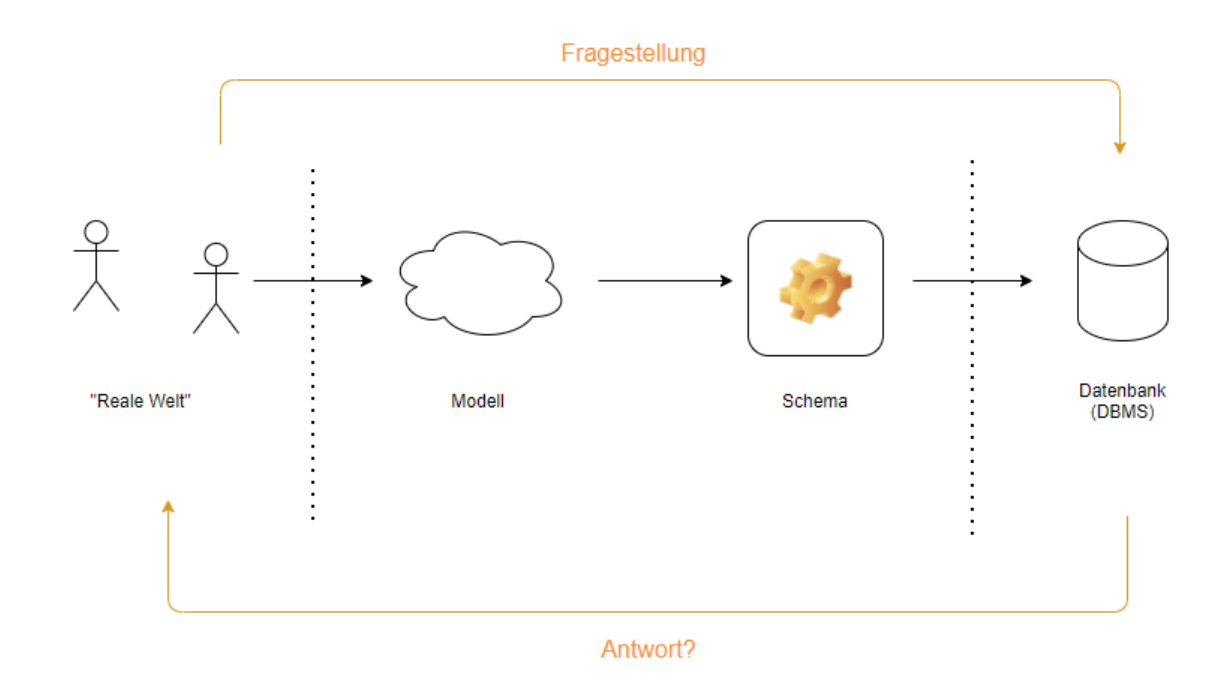
\includegraphics[width=\textwidth]{img/von-welt-zu-db.png}
\end{frame}

%------------------------------------------------------------------------------
\begin{frame}{Der Übergang zur Datenbank}
    % ----------------------------------------------
  \begin{columns}[T,onlytextwidth]
  \metroset{block=fill}
    \column{0.4\textwidth}\footnotesize
    \begin{block}{Datenanalyse Bsp: Tabelle aus Orten}
    \begin{itemize}
        \item Sind die Koordinatenpaare in der Tabelle einzigartig (oder gibt es Dopplungen)?
        \item Gruppiere und zähle die Orte nach Anzahl der Nachkommastellen des Längengrades etc. 
        \item Was gibt es für Abfragen an Visualisierungsmöglichkeiten?
    \end{itemize}
    \end{block}

    % ----------------------------------------------

    \column{0.55\textwidth}
      \metroset{block=fill}
      \begin{exampleblock}{Vorschau: Themenblock relationale Datenbanken}
      \begin{enumerate}\small
          \item  \textbf{Informations- und Datenmodellierung} = Der Weg in die Datenbank
          \item \textbf{Datenanalyse} = Informationen aus der Datenbank wieder herausholen, um Fragestellungen zu beantworten / Strukturierte Information repräsentiert durch Daten abfragen
      \end{enumerate} 
      \end{exampleblock}
  \end{columns}
\end{frame}

%------------------------------------------------------------------------------
\begin{comment}
\begin{frame}[standout]
    \alert{Lektüre} auf nächste Einheit: \\
    McCarty, Modelling
\end{frame}
\end{comment}

%------------------------------------------------------------------------------
\begin{frame}[standout]
    \alert{Hausübung:} Installation von \alert{\href{https://sqlitebrowser.org/dl/}{SQLite}} \\[1em]
    {\footnotesize
    \begin{enumerate}
        \item ggf. in Gruppen zusammenfinden nach Betriebssystem (Linux, Windows, Mac)
        \item wer es schon hat, kann gehen
        \item von mir aus braucht man nicht den Browser, sondern nur SQLite 
        \item wer es noch nicht hat, jetzt geht und dann doch Probleme hat, muss es sich selbst organisieren
        \item $\to$ Möglichkeit bei der Installation Hilfe zu bekommen, falls was nicht klappt
        \item \alert{Tutorials: \href{https://www.tutorialspoint.com/sqlite/sqlite_installation.htm}{Tutorialspoint} | \href{https://www.sqlitetutorial.net/download-install-sqlite/}{SQLiteTutorial} | \href{https://github.com/sqlitebrowser/sqlitebrowser}{SQLiteBrowser Github}}
    \end{enumerate}
    }
\end{frame}
 %DONE


\section{Data modelling II}
%------------------------------------------------------------------------------
\begin{frame}[standout]
    Re: \\ \alert{Data modelling} \\
    (but more technical now)
\end{frame}
%------------------------------------------------------------------------------
\begin{frame}{Data modelling}
\subsection{Definitions and theory}
\metroset{block=fill}
\begin{block}{Representation of originals (attributes)}
\begin{itemize}
    \item image (photo, drawing, diagram etc.)
    \item text 
    \item lists, tables
    \item audio 
    \item objects (experimental setup, sculpture, 3D print, etc.)
\end{itemize}
\end{block}


\begin{block}{What is data modelling?}
\begin{itemize}
    \item \textbf{data:} What does `data' mean?
    \item \textbf{modelling:} What does `data modelling' mean?
\end{itemize}
\end{block}

\end{frame}

%------------------------------------------------------------------------------
\begin{frame}[allowframebreaks]{Data}
\metroset{block=fill}
\begin{block}{Definitions of `data'}
    \begin{enumerate}\footnotesize
        \item Plural of Latin \emph{datum} ('given'): data often isn't exactly a given but a construct: data is created rather than given
        \item  \lbrack{}number\rbrack{}values, findings features, statements, details (collected/created through observation, measurement, statistical polls, phenomenotechnical devices)
        \item (IT) digital numbers, information 
        \item (maths) values given to solve an equation 
    \end{enumerate}
\end{block}

\begin{block}{ISO definitions = standard}\scriptsize
\begin{itemize}
    \item ISO/IEC 2382:2015(en): Information technology -- Vocabulary 2121272 data
    \item \textbf{Reinterpretable representation of information in a formalized manner suitable for communication, interpretation, or processing}
    \item Note 1 to entry: Data can be processed by humans or by automatic means (\href{https://www.iso.org/obp/ui/\#iso:std:iso-iec:2382:ed-1:v1:en}{source})
\end{itemize}
\end{block}

\framebreak
    \begin{block}{Data models}
    \begin{quote}
        Data models are models in the sense of Stachowiak's three main features of a mode but they have one more property: Models generally aren't necessarily computer-processable. To achieve this, they need to be given in an unambiguous, explicit way. Only then can they be machine-processed and only then are they formal models. 
        ~\parencite[100][translated from German]{JannidisIntroDatamod}
        %Datenmodelle sind Modelle in diesem Sinne \lbrack{}3 Hauptmerkmale nach Stachowiak\rbrack{}, aber es kommt eine weitere Eigenschaft hinzu. Modelle im Allgemeinen sind nicht automatisch von Computern prozessierbar. Um das zu erreichen, müssen sie in einer eindeutigen und expliziten Form vorliegen. Erst so können sie vom Computer verarbeitet werden und erst dann sind es formale Modelle. ~\parencite[100][translated from German]{JannidisIntroDatamod}
    \end{quote}
    \end{block}
\end{frame}

%------------------------------------------------------------------------------
\begin{frame}[allowframebreaks]{Digital data representation}
$\to$ i.e. \alert{computer processable}
\metroset{block=fill}
\begin{block}{Digital representation}
    \begin{itemize}
        \item \textbf{images} 
        \begin{itemize}
            \item raster graphics (\texttt{.png}, \texttt{.jpeg}) 
            \item vector graphics (\texttt{.svg})
        \end{itemize}
        \item \textbf{Text}
        \begin{itemize}
            \item plain text (\texttt{.txt})
            \item formatted text (\texttt{.docx})
        \end{itemize}
        \item \textbf{Lists, tables} (\texttt{.csv}, \texttt{.xlsx})
        \item \textbf{Audio} (\texttt{.wav}, \texttt{.midi})
        \item \textbf{Objects:} (Simulation of) three dimensionality and physical attributes
    \end{itemize}
\end{block}
\framebreak 

\begin{block}{For advanced froms of digital representation $\to$ see other ZIM classes}
\begin{itemize}
    \item \textbf{markup languages/OHCO} (\texttt{.xml}, etc.)
    \item \textbf{data objects} (\texttt{.json}, etc.) 
    \item \textbf{graph databases} (\texttt{.rdf}, etc.)
    \item \textbf{relational databases} $\to$ SQL (will follow soon\dots)
\end{itemize}
\end{block}
\end{frame}

%------------------------------------------------------------------------------
\begin{frame}{Fotis Jannidis' phases of data modelling}
\metroset{block=fill}
    \begin{alertblock}{1) conceptual data model}\footnotesize
        \begin{enumerate}
            \item identify relevant entities and their attributes and relations	$\to$ relevant concerning their intended use
            \item visualize entities, attributes and relations in a suitable format $\to$ lists, tables, diagrams (e.g. Entity Relationship Diagramm)
        \end{enumerate}
    \end{alertblock}
    \begin{alertblock}{2) logical data model}
        Map the conceptual model onto the structure of a specific technology, e.g. database schema or XML schema 
    \end{alertblock}
    \begin{alertblock}{3) physical data model}
        Implementation and physical representation of the data model in the memory of a computer as a specific data structure 
    \end{alertblock}
\end{frame}
%------------------------------------------------------------------------------
\begin{frame}{Jannidis, example diagram}
    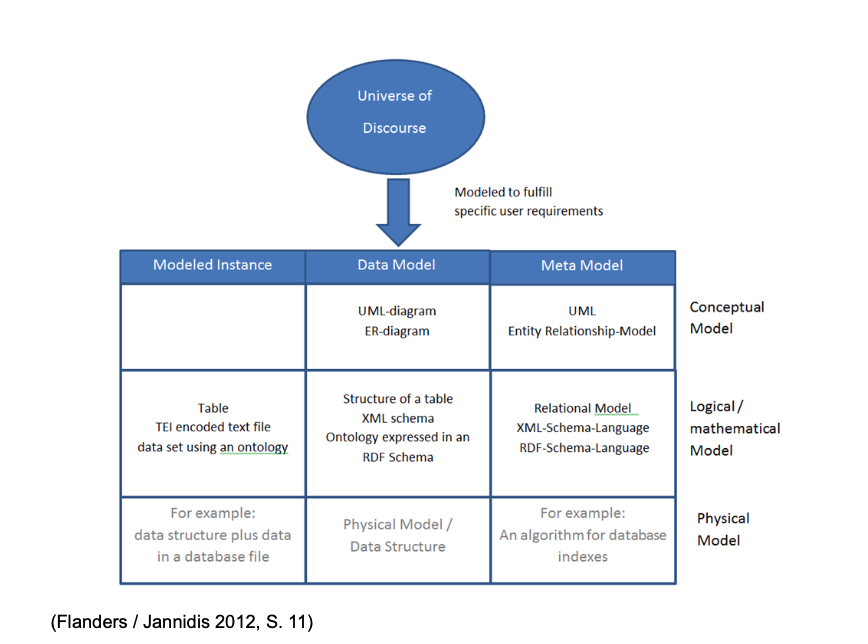
\includegraphics[width=\textwidth]{img/jannidis-modell.png}
\end{frame}

%------------------------------------------------------------------------------
\begin{frame}[fragile]{Example: csv data format (=comma separated values)}
\subsection{csv data format (=comma separated values \texttt{.csv})}
    \begin{enumerate}
        \item simple exchange format for sheet calculation software 
        \item cells (attributes) are separated by a separator character (such as comma, semicolon, tab, etc.)
        \item entries (datasets) separated by newline/line break
        \item fields can be named using headers (optional)
    \end{enumerate}
    \textbf{Source:} \protect\url{ietf.org}, \protect\url{https://tools.ietf.org/html/rfc4180}
    
    \metroset{block=fill}
    \begin{block}{csv example: birth place}\scriptsize
    \begin{verbatim}
    "Name","Address","Description","Longitude","Latitude"
    "forname surname","example street 1, postcode","birth place","7.018242","50.678667"
    \end{verbatim}
    \end{block}
\end{frame}



%------------------------------------------------------------------------------
\section{Entity Relationship Model (ERM)}
%------------------------------------------------------------------------------

%------------------------------------------------------------------------------
\begin{frame}{Entity Relationship Model (by Peter Chen)}
\metroset{block=fill}
\begin{block}{\cite[9]{chen1976}}
    \begin{quote}
        The entity-relationship model can be used as a basis for unification of different views of data: the network model, the relational model, and the entity set model.~
    \end{quote}
\end{block}
\begin{block}{\cite[10]{chen1976}}
    \begin{quote}
        \lbrack{}His article\rbrack{} analyzes the network model, the relational model, and the entity set model, and describes how they may be derived from the entity relationship model.~
    \end{quote}
\end{block}
\begin{block}{\cite[19]{chen1976}}
    \begin{quote}
        \lbrack{}The article presents:\rbrack{} a diagrammatic technique for exhibiting entities and relationships: the entity-relationship diagram.~%\parencite[19]{chen1976}
    \end{quote}
\end{block}
$\to$ \alert{Conceptual model}

\end{frame}

%------------------------------------------------------------------------------
\begin{frame}{ER terminology~\parencite[9--12]{chen1976}}
    % ----------------------------------------------
  \begin{columns}[T,onlytextwidth]
  \metroset{block=fill}
    \column{0.55\textwidth}\footnotesize
      \begin{block}{Entity (Entität)}
       An entity is a „thing“ which can be distinctly identified. A specific person, company, or event is an example of en entity.
      \end{block}

      \begin{alertblock}{Relationship (Beziehung)}
        A relationship is an association among entites. For instance, „father-son“ is a relationship between two „person“ enitities.
      \end{alertblock}

      \begin{exampleblock}{Entity Set (Entitätsmenge)}
        All entities of the same entity set have the same properties.
        %Alle Entitäten derselben Entitätsmenge haben dieselben Eigenschaften (properties). 
        
        „Entities are classified into different entity sets such as EMPLOYEE, PROJECT, and DEPARTMENT.“
      \end{exampleblock}

    % ----------------------------------------------

    \column{0.4\textwidth}

      \metroset{block=fill}

      \begin{block}{ER model elements}
      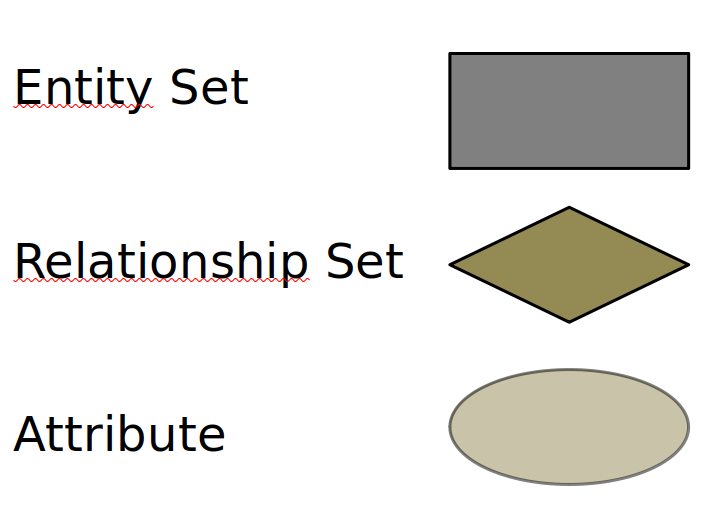
\includegraphics[width=0.9\textwidth]{img/er-modell.png}
      \end{block}
      
      \begin{block}{ER elements}
      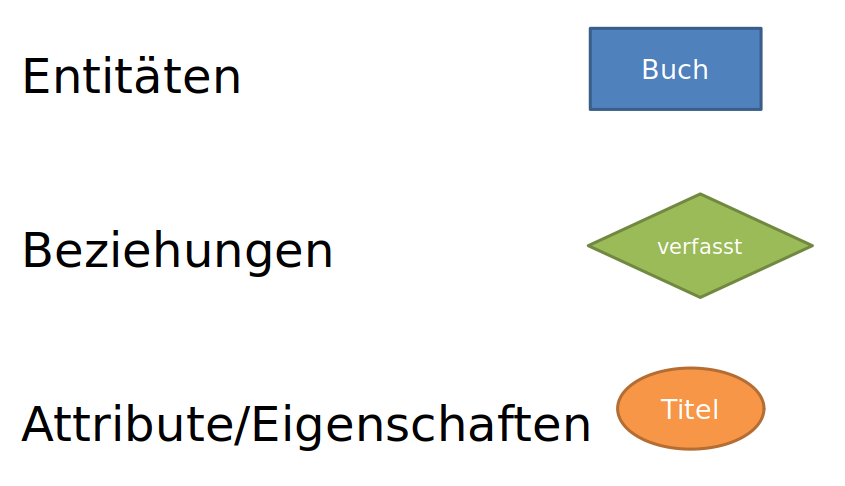
\includegraphics[width=0.9\textwidth]{img/er-bsp2.png}
      \end{block}
  \end{columns}

\end{frame}

%------------------------------------------------------------------------------
\begin{frame}{ER terminology~\parencite[9--12]{chen1976}}
    % ----------------------------------------------
  \begin{columns}[T,onlytextwidth]
  \metroset{block=fill}
    \column{0.48\textwidth}\footnotesize
      \begin{exampleblock}{set of relations (Relationship Set)}
        Same relationships between entities from the same entity sets: can be summarized in a set of relationships.
        %Gleiche Beziehungen zwischen Entitäten, die jeweils aus derselben Entitätsmenge stammen, lassen sich in einer Menge von Beziehungen zusammenfassen. 
      \end{exampleblock}

    % ----------------------------------------------

    \column{0.48\textwidth}

      \metroset{block=fill}
      \begin{block}{Role (Rolle)} \footnotesize
        The role of an entity in a relationship is the function that it performs in the relationship.
      \end{block}
      
      \begin{alertblock}{Properties (Eigenschaften)}\footnotesize
        Using properties, entities and relationships can be described. 
        %Mithilfe von Eigenschaften lassen sich Entitäten (Entities) und Beziehungen (Relationships) beschreiben. 
      \end{alertblock}
  \end{columns}
  \begin{center}
      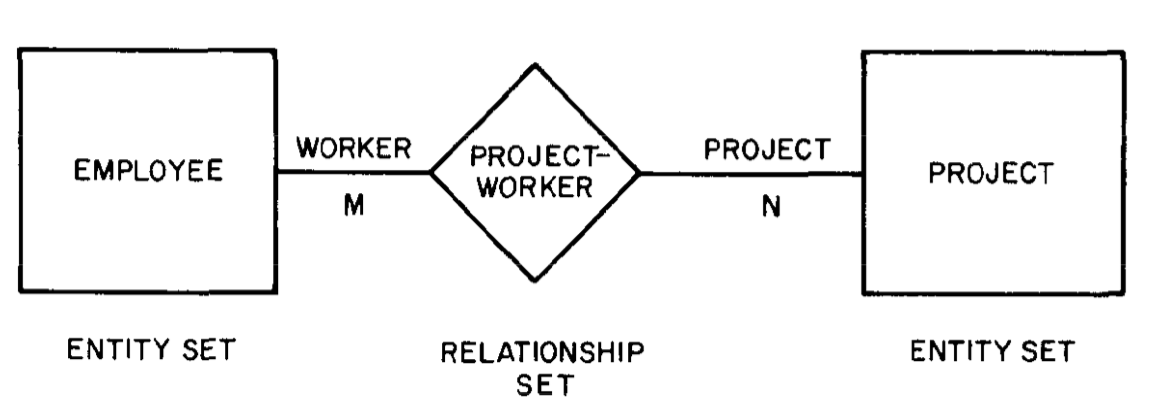
\includegraphics[width=0.6\textwidth]{img/er-bsp.png}
  \end{center}
\end{frame}


%------------------------------------------------------------------------------
\begin{frame}{ER example for a book}

\footnotesize
\begin{tikzpicture}[node distance=6.5em]
%--------------------
% the book
%--------------------
\node[entity](book){Book};
\node[attribute](isbn)[left of=book]{\key{ISBN}} edge(book);
\node[attribute](title)[above left of=book]{title} edge(book);
\node[attribute](pagenr)[above of=book]{nr. of pages} edge(book);

%--------------------
% published by publisher
%--------------------
\node[relationship](published)[below of=book, yshift =-2em]{published} edge node[above right]{N}(book);
\node[entity](publisher)[below of=published, yshift =-2em]{publisher} edge node[above right]{1}(published);
\node[attribute](tid)[left of=publisher]{\key{ID}} edge(publisher);
\node[attribute](tname)[right of=publisher]{Name} edge(publisher);
\node[attribute](address)[above right of=publisher]{address} edge(publisher);
\node[attribute](street)[above right of=address]{Street} edge(address);
\node[attribute](city)[right of=address]{City} edge(address);
\node[multi attribute](phonenr)[below right of=publisher]{phone number} edge(publisher);

%--------------------
% written by author
%--------------------
\node[relationship](written)[right of=  book, xshift =3em]{written} edge node[above right]{N}(book);
\node[entity](author)[right of= written, xshift =3em]{author} edge node[above right]{M}(written);
\node[attribute](birthday)[above  of=author]{birthday} edge(author);
\node[attribute](name)[above right of=author]{name} edge(author);
\node[derived attribute](age)[right of=author]{Age} edge(author);
\end{tikzpicture}

\framebreak 

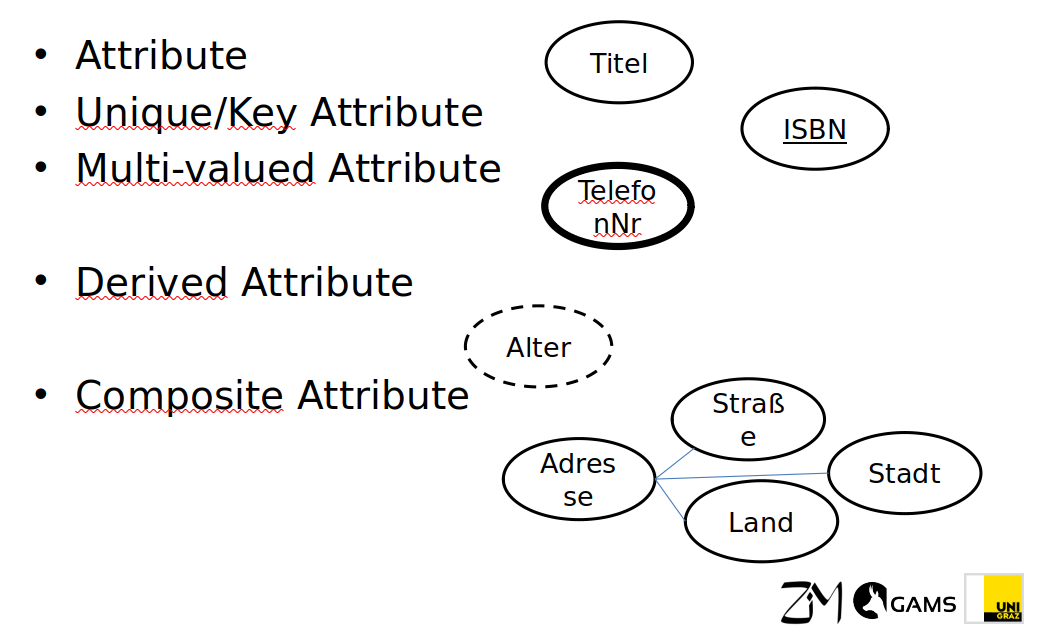
\includegraphics[width=\textwidth]{img/wdh-er-bestandteile.png}

\end{frame}

%------------------------------------------------------------------------------
\begin{frame}{ER example for a book}
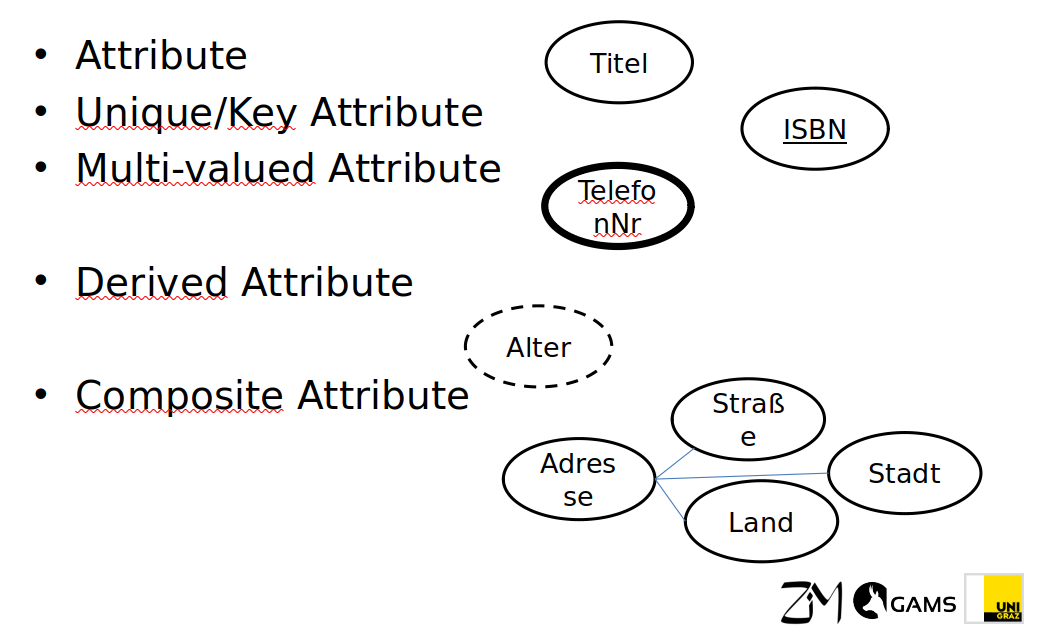
\includegraphics[width=\textwidth]{img/wdh-er-bestandteile.png}

\end{frame}



%------------------------------------------------------------------------------
\begin{frame}[fragile]{Examples}
\metroset{block=fill}
\begin{block}{Entities: university class}
    \begin{itemize}
        \item \textbf{entities:} class, teacher, students, room 
        \item \textbf{attributes:} class (nr., title), teacher (name), students (name, student nr, degree programme, module), room (nr, building, seats) 
        \item \textbf{relations:}
        \begin{itemize}
            \item Teacher teaches class. Ein Kurs wird abgehalten von Dozent:in.
            \item Class happens in room.
            \item Students participate in class. 
        \end{itemize}
    \end{itemize}
\end{block}

\begin{block}{csv example: birth place}\scriptsize
    \begin{verbatim}
    "Name","Address","Description","Longitude","Latitude"
    "forname surname","example street 1, postcode","birth place","7.018242","50.678667"
    \end{verbatim}
    \end{block}
\end{frame}
%------------------------------------------------------------------------------
\begin{frame}{Homework: CSV}
\metroset{block=fill}
    \begin{alertblock}{Assignment}
    \begin{enumerate}\footnotesize
        \item Represent attributes (properties and relations) of your original in a computer processable table (\texttt{.csv} file).
        %Repräsentieren Sie die Attribute (Eigenschaften und Relationen) Ihres Originals mithilfe einer vom Computer zu verarbeitenden Tabelle (CSV-Datei).
        \item To do that, put your attributes in a simple text-only file in a simple text editor (don't do this in MS Word or the like!), saving the file as \texttt{.txt} or \texttt{.csv} (UTF-8 encoding) or export from a table/sheet software like GoogleSheets, LIbre/OpenOffice Calc or Excel. 
    \end{enumerate}
\end{alertblock}

\begin{block}{Please note:}\tiny
Keep in mind that you can only represent attributes in a limited way using CSV:

You can representt the type of relatinship (e.g. `made of', `instance-class-relationship', `bigger-than', etc.) using suitable labels in the CSV header and true/false answers as values for the cells -- but you can't (at this point) say which relationships link entities (such as molecule -- made of -- H).

Relational databases allow for this more complete form of representation between entities using their relationships. For this homework, picking something that will easily fit in to this list / Excel sheet type format will suffice. 
\end{block}
\end{frame}


%------------------------------------------------------------------------------
\begin{frame}[standout]
    \alert{Action!} \\
    Let's install SQLite3 and try out the terminal.
\end{frame}



\section{ER models (repetition \& continuation)}

%------------------------------------------------------------------------------
\begin{frame}{Repetition: ER terminology~\parencite[9--12]{chen1976}}
    % ----------------------------------------------
  \begin{columns}[T,onlytextwidth]
  \metroset{block=fill}
    \column{0.55\textwidth}\footnotesize
      \begin{block}{Entity (Entität)}
       An entity is a „thing“ which can be distinctly identified. A specific person, company, or event is an example of en entity.
      \end{block}

      \begin{alertblock}{Relationship (Beziehung)}
        A relationship is an association among entites. For instance, „father-son“ is a relationship between two „person“ enitities.
      \end{alertblock}

      \begin{exampleblock}{Entity Set (Entitätsmenge)}
        All entities of the same entity set have the same properties.
        %Alle Entitäten derselben Entitätsmenge haben dieselben Eigenschaften (properties). 
        
        „Entities are classified into different entity sets such as EMPLOYEE, PROJECT, and DEPARTMENT.“
      \end{exampleblock}

    % ----------------------------------------------

    \column{0.4\textwidth}

      \metroset{block=fill}

      \begin{block}{ER model elements}
      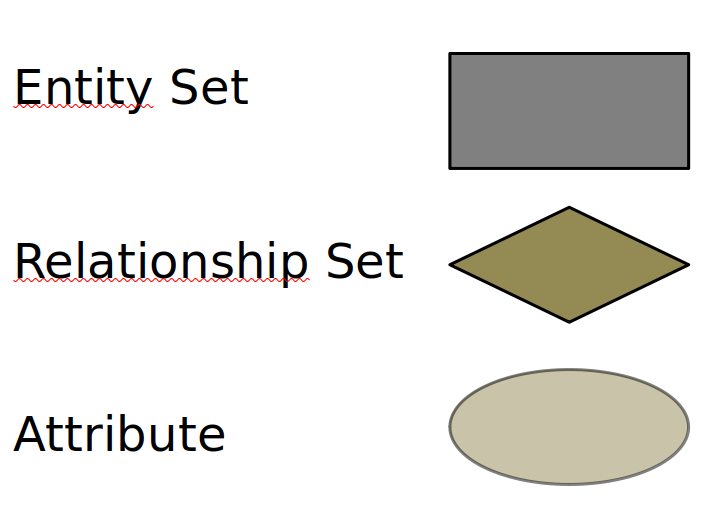
\includegraphics[width=0.9\textwidth]{img/er-modell.png}
      \end{block}
      
      \begin{block}{ER elements}
      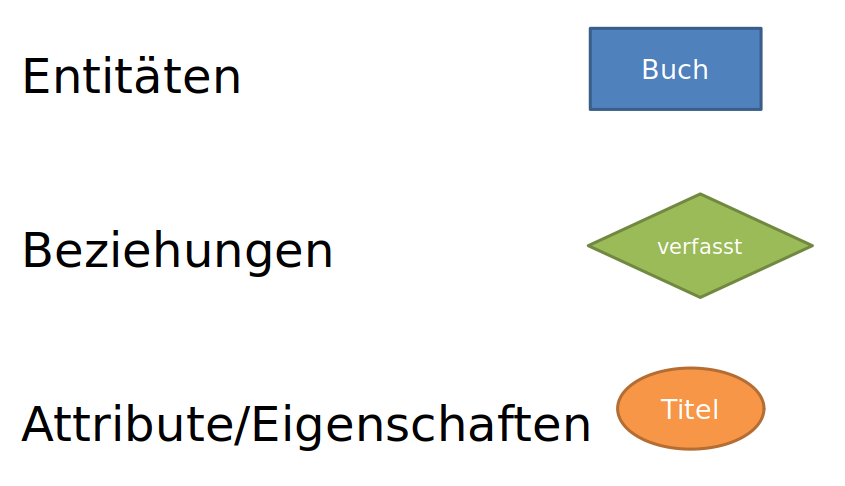
\includegraphics[width=0.9\textwidth]{img/er-bsp2.png}
      \end{block}
  \end{columns}

\end{frame}

%------------------------------------------------------------------------------
\begin{frame}{Repetition ER}
    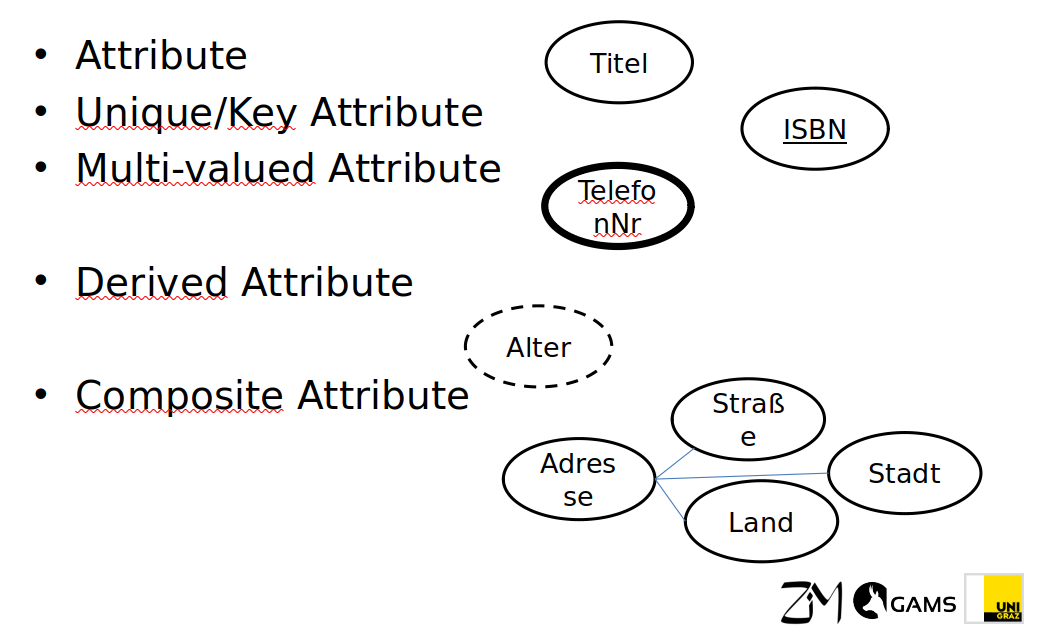
\includegraphics[width=\textwidth]{img/wdh-er-bestandteile.png}
\end{frame}


%------------------------------------------------------------------------------
\begin{frame}{Attribute values pairs and Primary Keys}
    Properties (Eigenschaften) are expressed by a attribute-value combination like so: 
    \begin{enumerate}
        \item The pen is blue = The `pen' entity has the attribute `color' with the value `blue'. 
        \item The pen is red = The `pen' entity has the attribute `color' with the value `red'. 
    \end{enumerate}

\metroset{block=fill}
\begin{exampleblock}{Primary Key: Identifying properties}
Entities and relationships can be uniquely identified via the value of one or multiple attributes combined. This attribute / the attribute combination is then called `primary key'. 
\end{exampleblock}
\end{frame}
%------------------------------------------------------------------------------
%\begin{frame}{Beispiel ER-Modell für ein Buch}    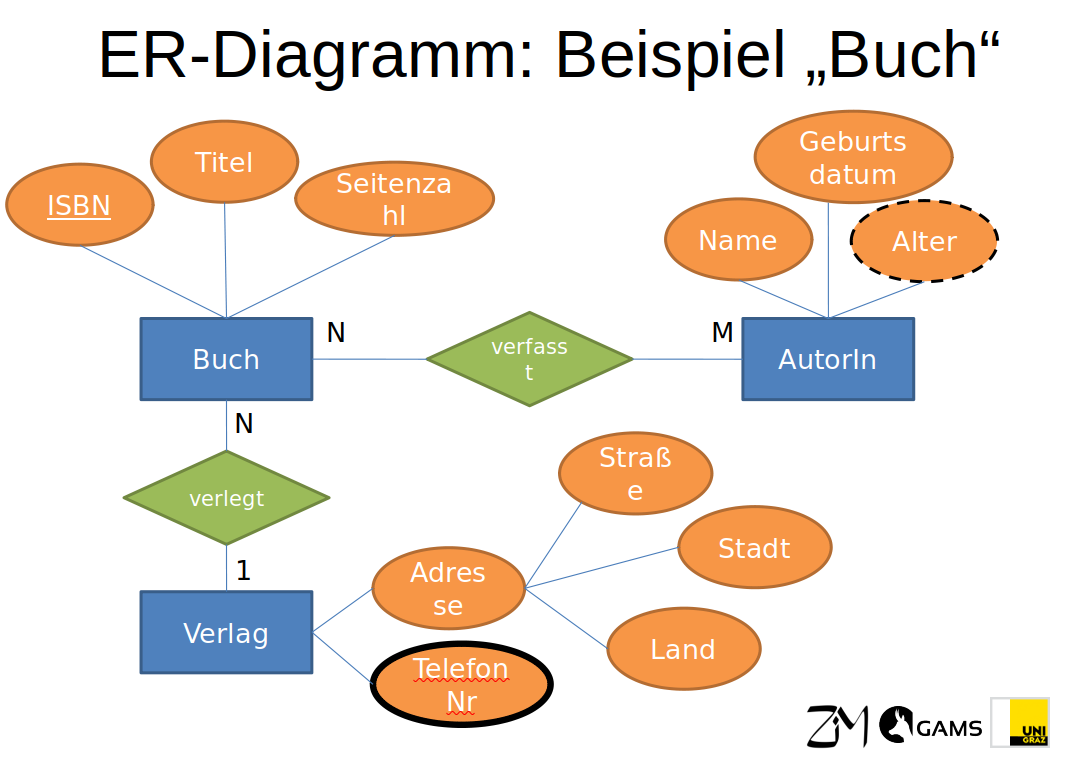
\includegraphics[width=\textwidth]{img/er-bsp3.png}\end{frame}


%------------------------------------------------------------------------------
\begin{frame}{Repetition exercise}
    % ----------------------------------------------
  \begin{columns}%[T,onlytextwidth]
  \metroset{block=fill}
    \column{0.45\textwidth}\footnotesize
    \begin{block}{A session of a university course}
    Such a session is defined by having:
    \begin{enumerate}
        \item students
        \item teachers
        \item seats
        \item a room
        \item in a building
    \end{enumerate}
    \end{block}

    % ----------------------------------------------

    \column{0.55\textwidth}
      \metroset{block=fill}\footnotesize
      \begin{exampleblock}{Exercise 1}
      \begin{enumerate}
          \item Which attribute can be used to describe these entities? %Mit welchen Attributen lassen sich diese Entitäten beschreiben?
          \item Using which attributes can the entities be uniquely identified? %Anhand welcher Attribute lassen sich die Entitäten jeweils identifizieren?
          \item Which relationships do they have amongst each other? %Welche Beziehungen existieren zwischen den Entitäten?
      \end{enumerate}
      $\to$ related to a normal in-person class % bezogen auf normalen Präsenzunterricht
      \end{exampleblock}
      \begin{exampleblock}{Exercise 2}
      How do we have to change this to accomodate distance learning or even a hybrid setting? % Wie müsste man das jetzt umändern, um auch Distance Learning einzukalkulieren?
      \end{exampleblock}
      \footnotesize
      $\to$ do this exercise in groups/pairs and create a visualisation of the results, for example using \href{https://erdplus.com/standalone}{the erdplus.com tool} (be ready to present this briefly) % Übung in Gruppen. Erstellen Sie, wenn möglich, eine Zeichnung / einen Screenshot der Resultate, der dann vorgestellt wird.
  \end{columns}

\end{frame}


%------------------------------------------------------------------------------
\begin{frame}{Solution: class session in ER (in-person) }
    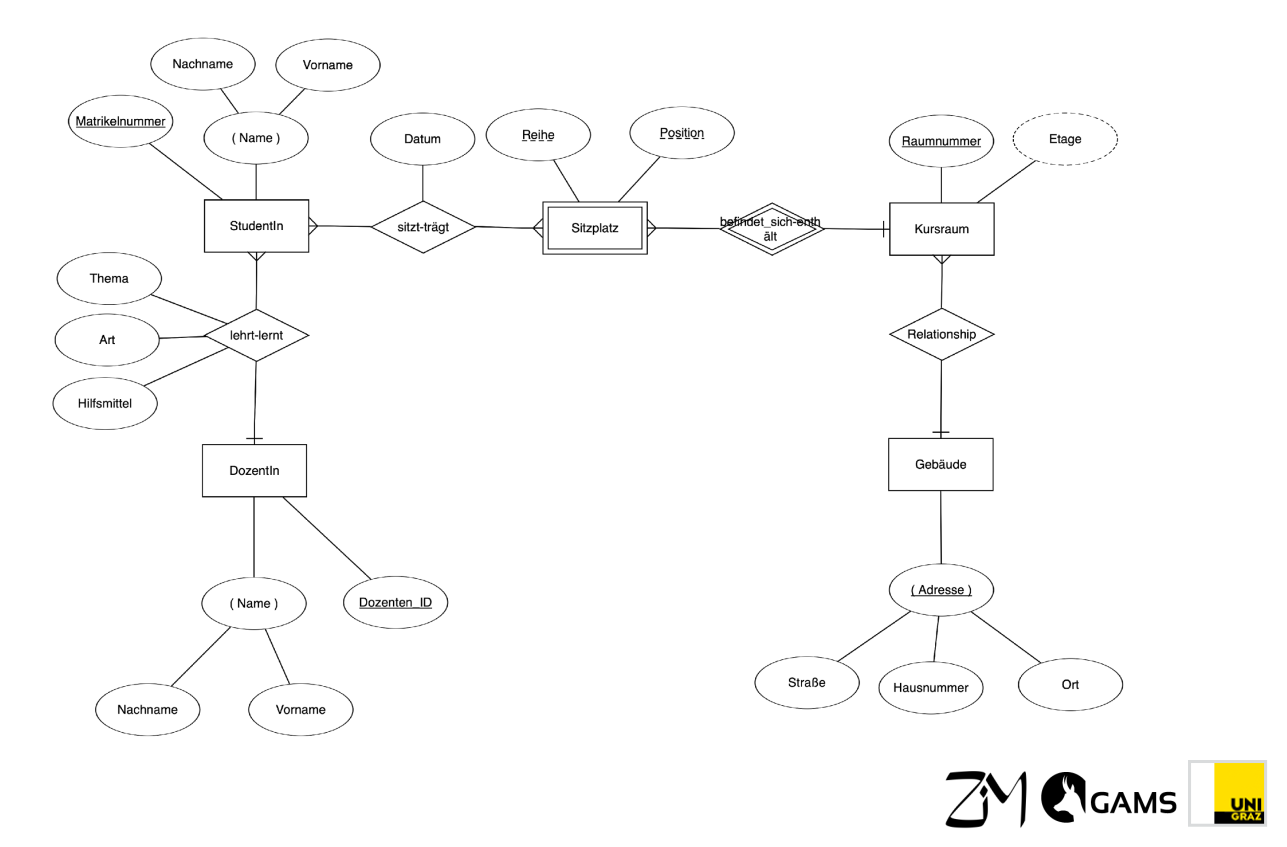
\includegraphics[width=\textwidth]{img/wdh-er-kursmodellierung.png}
\end{frame}


\subsection{ERM -- Tables \& relations}
%------------------------------------------------------------------------------

%------------------------------------------------------------------------------
\begin{frame}{From ER model to table format?}
    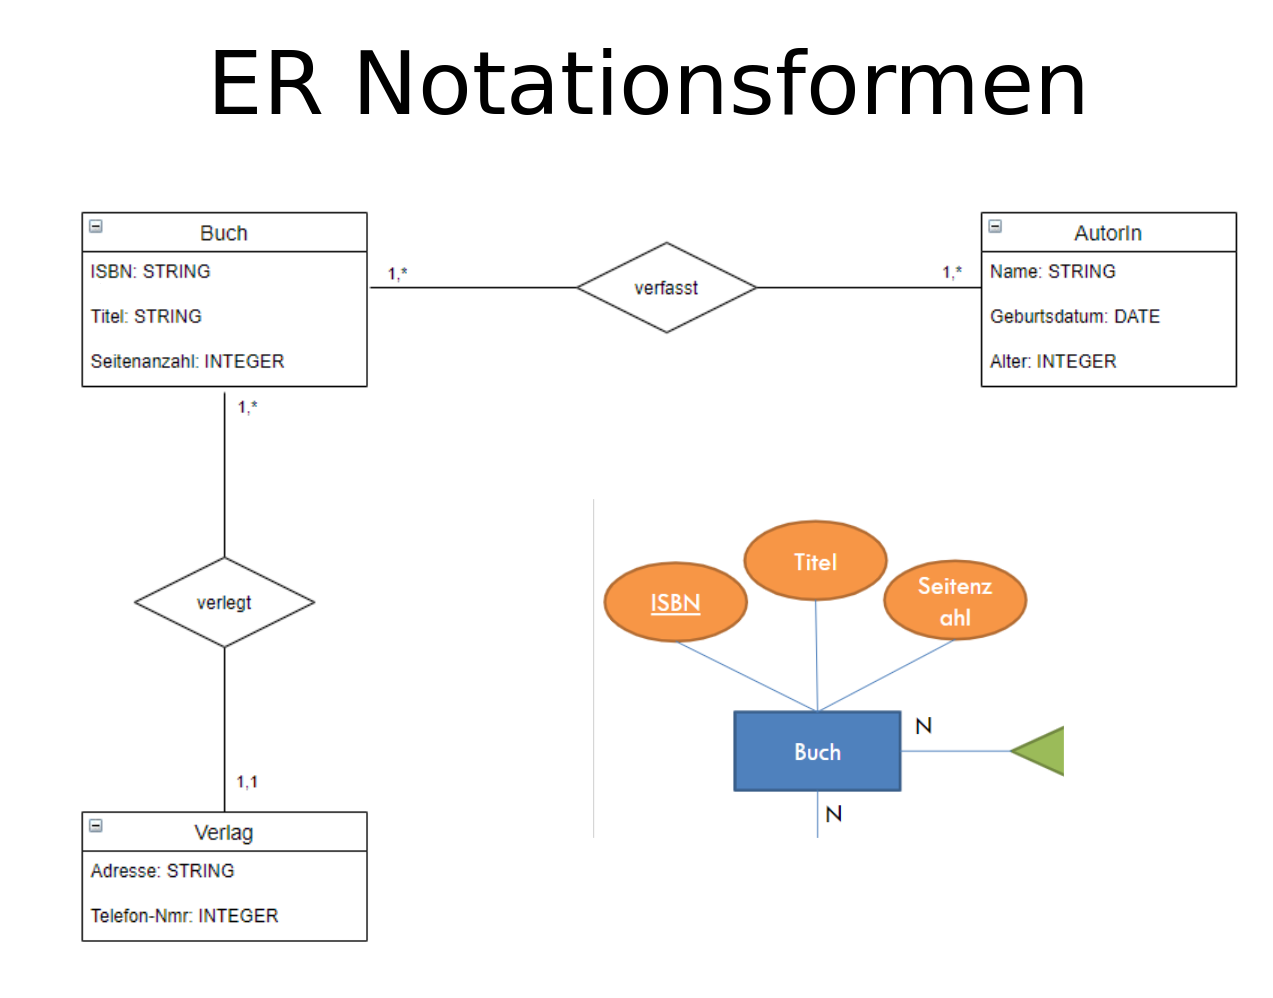
\includegraphics[width=\textwidth]{img/er-notation-buch.png}
\end{frame}

%------------------------------------------------------------------------------
\begin{frame}{Representation of ER models as tables}
    % ----------------------------------------------
  \begin{columns}[T,onlytextwidth]
  \metroset{block=fill}
    \column{0.4\textwidth}\footnotesize
    \begin{block}{Representation as tables}
    Entities and their relationships can be represented as tables. \\
    But where to put the attributes? 
    
    \end{block}

    % ----------------------------------------------

    \column{0.55\textwidth}
      \metroset{block=fill}
      \begin{exampleblock}{Handeling cardinalities}
      \begin{enumerate}\small
          \item Same book, multiple authors? (Why not just as an attribute?) 
          \item Same book, multiple genres? (entity or attribute?) 
          \item How to model the content of the book? (if at all?)
      \end{enumerate} \small
      $\to$ keep these questions in mind for a discussion later (on cardinality)
      \end{exampleblock}

  \end{columns}
\end{frame}

%------------------------------------------------------------------------------
\begin{frame}{Transform entities \& attributes to tables: e.g. class}
    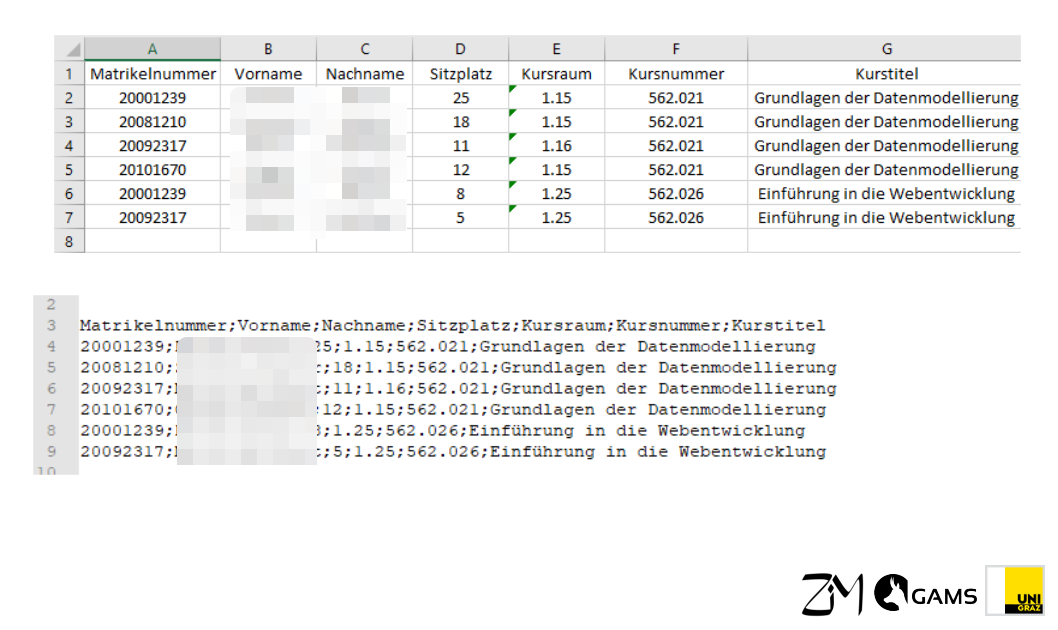
\includegraphics[width=\textwidth]{img/wdh-studierende-csv.png}
\end{frame}


%------------------------------------------------------------------------------
%\begin{frame}[standout]
    %\alert{Lektüre}-Zusammenfassung: \\
    %Chen, ER-Modelle \\[1em]
    %{\footnotesize Bitte \alert{\href{https://docs.google.com/presentation/d/1v_j9Jms21hZokX9hLJ_7kcnV63FJPHTHNowfLVLiYys/edit?usp=sharing}{hier im Google Slides zusammenfassen}}; 1 Person stellt dann vor. \\
    %Themen 1 und 2 für jene ohne größere DB-Vorwissen; 3 und 4 bitte möglichst, falls schon gewisses Programmierungs-/DB-Wissen vorhanden ist. \\
    %Aufgabe ist nicht, Details herauszupicken -- stark Technisches kann man auch weglassen. \alert{Bitte um Fokus auf die Verständnis-Aspekte.} Man kann gern zur Hilfe andere Materialien dazunehmen. Versuchen, den Mitstudierenden den Text möglichst verständlich aufzubereiten/zusammenzufassen. \\
    %Zeit ca. 20min}
%\end{frame}

%------------------------------------------------------------------------------
\begin{frame}{From real-world object to relational database?}
    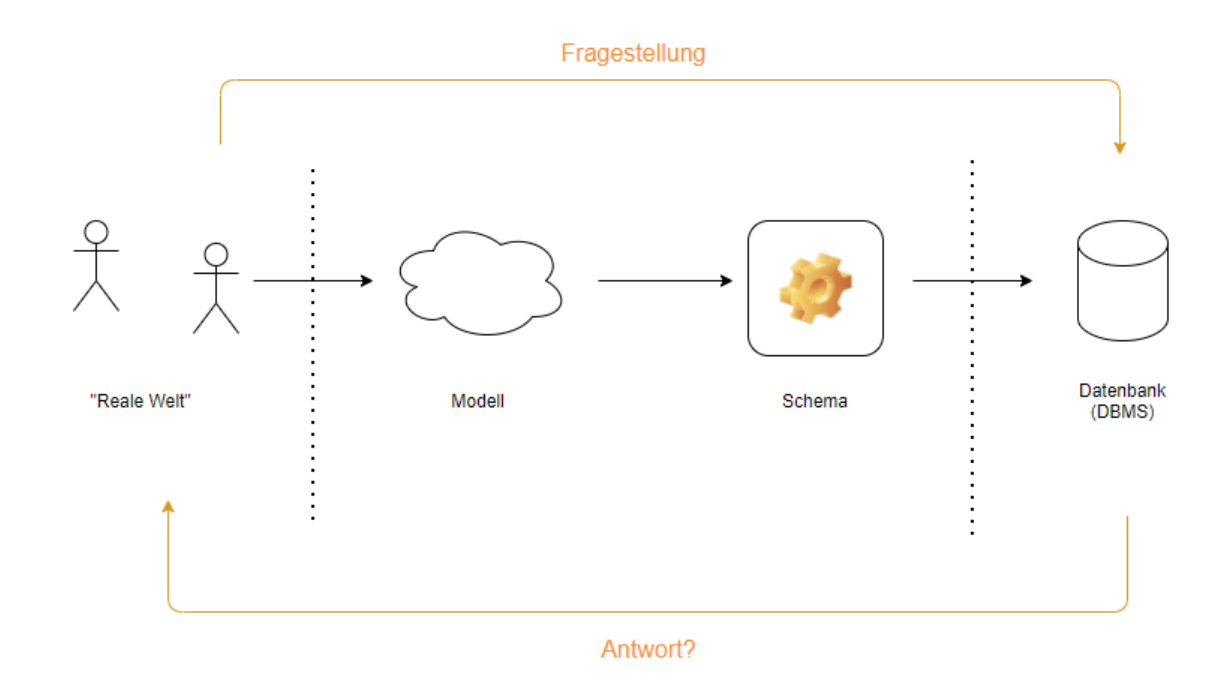
\includegraphics[width=\textwidth]{img/von-welt-zu-db.png}
\end{frame}

%------------------------------------------------------------------------------
\begin{frame}{Moving towards databases\dots}
    % ----------------------------------------------
  \begin{columns}[T,onlytextwidth]
  \metroset{block=fill}
    \column{0.4\textwidth}\footnotesize
    \begin{block}{Data analysis example: table of places}
    \begin{itemize}
        \item Are coordinates unique in the table or do some appear more than once? 
        \item Group and count places using the last digits of the latitude values, etc. 
        \item What visualizations would work for this data?
    \end{itemize}
    \end{block}

    % ----------------------------------------------

    \column{0.55\textwidth}
      \metroset{block=fill}
      \begin{exampleblock}{Preview: Relational Databases}
      \begin{enumerate}\small
          \item  \textbf{information and data modelling} = the way into the database
          \item \textbf{data analysis and retrieval} = query/retrieve information from the DB to answer questions: query structured data 
      \end{enumerate} 
      \end{exampleblock}
  \end{columns}
\end{frame}


%------------------------------------------------------------------------------
\begin{frame}[standout]
    \alert{Homework:} Install \alert{\href{https://sqlitebrowser.org/dl/}{SQLite}} \\[1em]
    {\footnotesize
    \begin{enumerate}
        \item maybe work in groups with those sharing your operating system (Linux, Windows, Mac)
        \item if you already have it, you can leave early -- but then figure it out yourself
        \item we don't necessarily need SQLiteBrowser (sometimes causes trouble)
        \item $\to$ there are tutorials; you can ask me or the others
        \item \alert{Tutorials: \href{https://www.tutorialspoint.com/sqlite/sqlite_installation.htm}{Tutorialspoint} | \href{https://www.sqlitetutorial.net/download-install-sqlite/}{SQLiteTutorial} | \href{https://github.com/sqlitebrowser/sqlitebrowser}{SQLiteBrowser Github}}
    \end{enumerate}
    }
\end{frame}



%------------------------------------------------------------------------------
%\begin{frame}[standout]
    %\alert{Reading:} \\ \small Bitte formieren Sie sich in Grupppen. Jede Gruppe erarbeitet eine Zusammenfassung eines Unterpunkts der Lektüre \alert{\href{https://docs.google.com/presentation/d/12w3XqjDO0IsLFwT0aFYiWED08WupCPxaswAEaxhqmuY/edit?usp=sharing}{in diesem GoogleDoc}} (Kapitel \emph{Grundlagen der Datenmodellierung}). \\ Jede Gruppe hat dafür max. 1 Slide zur Verfügung. Eine Person aus der Gruppe stellt diese am Ende dem Plenum vor. 
%\end{frame}


%------------------------------------------------------------------------------
%\begin{frame}[standout]
    %\alert{Reading} for next week: \\
    %DH-Einführung, Kapitel \emph{Datenmodellierung}
%\end{frame}

%------------------------------------------------------------------------------


%------------------------------------------------------------------------------
\begin{frame}{(materials for the) homework assignment}
\metroset{block=fill}
\begin{exampleblock}{Resources}
    \begin{itemize}\footnotesize
        \item \href{https://erdplus.com/standalone}{Tool for creating ER models}
        \item \href{https://www.geeksforgeeks.org/introduction-of-er-model/}{GeeksforGeeks tutorial/Intro to ER Models}
        \item \href{https://geobrowser.de.dariah.eu/}{DARIAH Geobrowser}
        \item \href{https://www.cloudbakers.com/blog/everything-you-didnt-want-to-have-to-know-about-csv}{Everything you didn't want to know about CSV}
    \end{itemize}
\end{exampleblock}

\begin{alertblock}{ER model homework assignment}
    \begin{enumerate}\footnotesize
        \item Create and visualize the model for your original (attribute class) using an ER diagram (like ERDplus) %Konzipieren und visualisieren Sie das Model Ihres Originals (Attributklasse) mithilfe des Entity-Relationship-Diagramms. (z.B. ERDplus siehe oben)
        \item Export it as an image and upload it on Moodle %Exportieren Sie ihr Diagramm als Bild und laden es auf Moodle hoch.
        \item In case of problems, help each other via Slack or in-person. %Bei Problemen können Sie sich auch gegenseitig im Hilfe-Forum unterstützen.
        \item \textbf{Bonus:} Look into the subject of cardinality and work it into your model. %Schauen Sie sich das Thema `Kardinalität' an bzw. erarbeiten es sich aus den Unterlagen und bauen Sie es in Ihr Modell ein. 
    \end{enumerate}
\end{alertblock}
\end{frame}

%------------------------------------------------------------------------------
%\begin{frame}[standout]
    %\alert{Lektüre} auf nächste Einheit: \\
    %Chen, ER-Modelle 
%\end{frame}


%------------------------------------------------------------------------------
\section{Cardinality}
\begin{frame}[allowframebreaks]{Cardinalities}
\metroset{block=fill}
    "cardinality" =  the number of entities participating in a relationship where  \textit{n} \& \textit{m} stand for an arbitrary number.

\begin{block}{Types of relationships}
 \textbf{1:1} $\to$ exactly one entity participates in the relationship. %Es gibt genau je eine Entität, die an der Beziehung beteiligt ist.
 
 \textbf{1:n} $\to$ There can be an arbitrary number of entities (on the n-side) for each single entity on the 1-side. %Für jede Entität auf der 1-Seite der Beziehung kann es beliebig viele Entitäten auf der n-Seite geben.
 
 \textbf{n:m} $\to$ There can be an arbitrary number for each entity on the n-side on the m-side and vice versa. %Für jede Entität auf der n-Seite der Beziehung kann es beliebig viel Entitäten auf der m-Seite geben und umgekehrt.
\end{block}

\begin{center}
  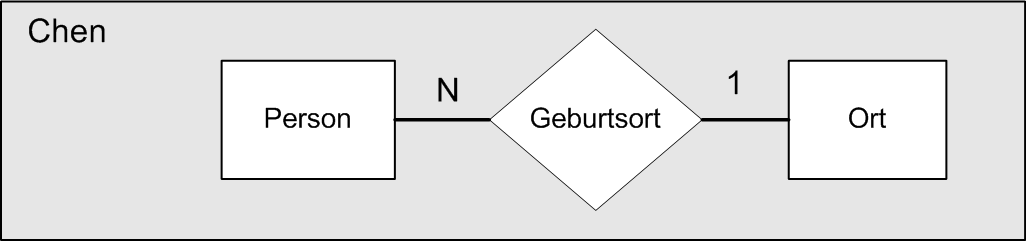
\includegraphics[width=0.7\textwidth]{img/ERD_Darstellungen_Chen.png}
\end{center}

\framebreak
\begin{block}{Minimal cardinalities} 
\textbf{0} $\to$ there doesn't have to be an entity on this side of the relationship. (=\textit{optional})

\textbf{1} $\to$ There has to be at least one entity on this side of the relationship.  (=\textit{obligatory})
\end{block}

\begin{center}
    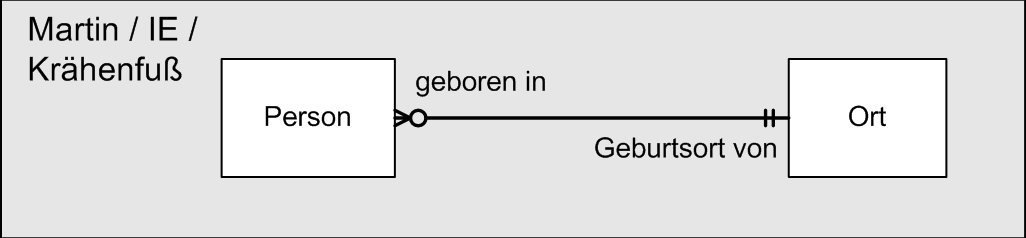
\includegraphics[width=0.7\textwidth]{img/ERD_Darstellungen_Crowfoot.png}
    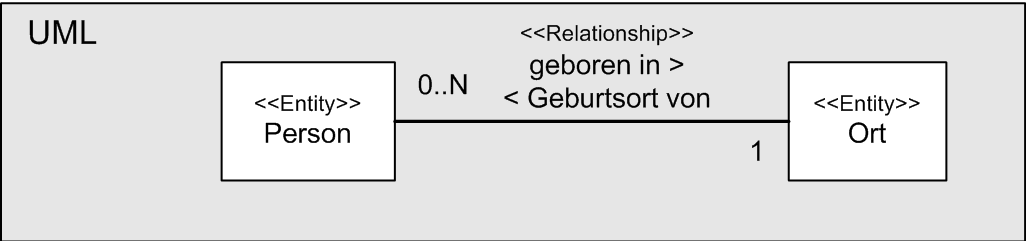
\includegraphics[width=0.7\textwidth]{img/ERD_Darstellungen_UML.png}
\end{center}

\end{frame}



%------------------------------------------------------------------------------
\begin{frame}{ER advanced}
    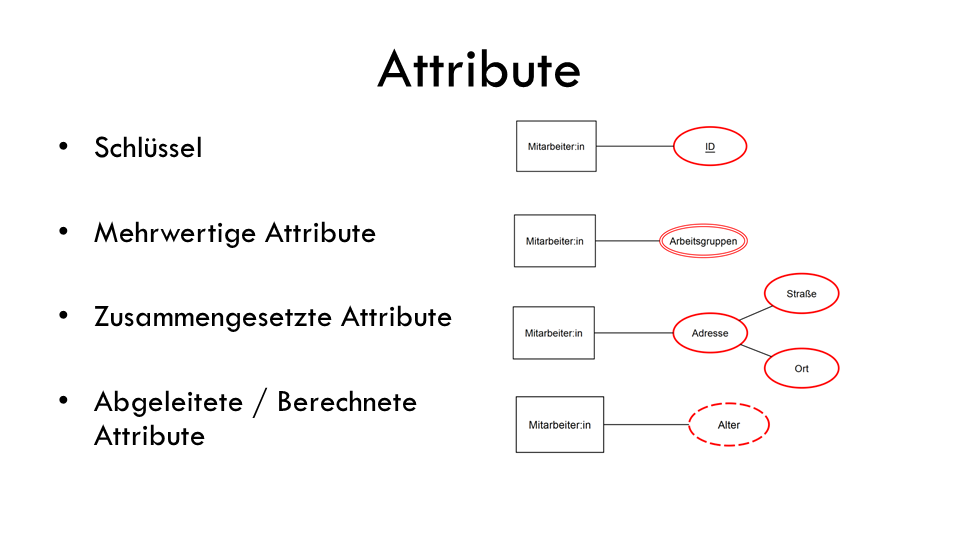
\includegraphics[width=\textwidth]{img/attribute.png}
\end{frame}


%-------------------------------------------------
\begin{frame}[allowframebreaks]{ER advanced}
    \begin{itemize}
        \item \textbf{identifying attributes (``keys``)}: these values are unique within the entity class and can thus be used to identify single entities. 
        \item \textbf{multivalued attributes}: attributes containing more than one atomic value.
        \item \textbf{derived attributes}: attributes which can be calculated from other attributes.
        \item \textbf{composite attributes}: attributes consisting of multiple parts.
    \end{itemize}
    
    \framebreak
    
    \begin{itemize}
        %\item \textbf{Attribute von Beziehungen}: Auch Beziehungen können Attribute haben.
        \item \textbf{n-ary relationships}: a relationship set can connect multiple entity sets (in principle). 
        \item \textbf{weak entity}: can only exist if there is a relation to another entity (room in building) but the key depends on the key of another relationship (Chen notation: double border). They have no properties of their own by which they can be identified (have no primary key). They are defined only by their relationship to a strong entity. Example: relatives of an employee in a company.
    \end{itemize}
\end{frame}
%\end{comment}

%-------------------------------------------------
    
\begin{frame}{n-ary relationships}
\begin{center}
    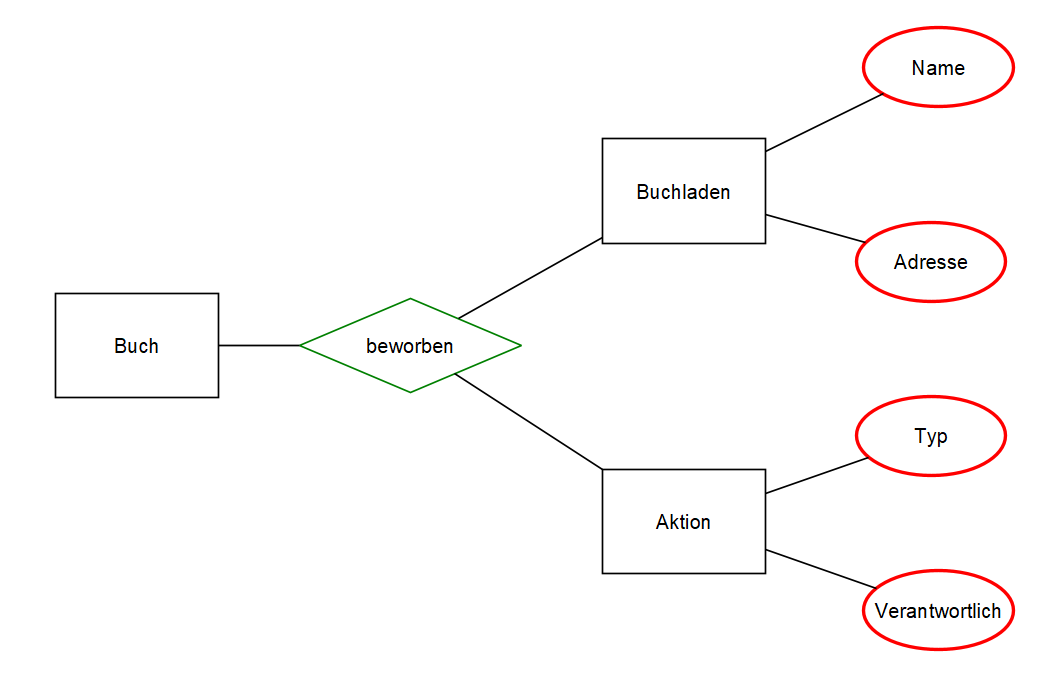
\includegraphics[width=0.9\textwidth]{img/n-ary-relationship.png}
\end{center}    
\end{frame}

%------------------------------------------------------------------------------
\begin{frame}{How to represent entities going from ER to table?}
    \begin{itemize}
        \item \textbf{entity} $\to$ table
        \item \textbf{attribute} $\to$ column
        \begin{itemize}
            \item multi-valued attributed $\to$ helper table
        \end{itemize}
        \item \textbf{relationship}
            \begin{itemize}\footnotesize
                \item \textbf{1:1} $\to$ Key of one entity (table) is stored as reference (`foreign key'/`Fremdschlüssel') in the other table as a column/attribute of its own 
                \item \textbf{1:n} $\to$ key of the 1-ary entity/table stored as reference in the n-ary table/entity 
                \item \textbf{n:m} $\to$ table of its own containing the keys of both related entities
                \item \textbf{n-ary relations} $\to$ helper table containing the keys of all entities as columns 
                \item \textbf{relationship attributes} $\to$ helper table with the keys of participating entities and columns for the attributes 
                \item \textbf{multi-valued attributes} $\to$ helper table with entity key as foreign key (like a 1:n relation) and a column for the attribute 
                \item \textbf{composite attributes} $\to$ helper table with entity key as foreign key (like a 1:n relation) and columns for the partial attributes 
            \end{itemize}
    \end{itemize}
\end{frame}


\section{Using the commandline / terminal}
% ----------------------------------
\begin{frame}[fragile,allowframebreaks]{Terminal/Commandline basics}
\footnotesize
\metroset{block=fill}

\begin{columns}
\column{0.55\textwidth}

\begin{block}{Navigating in the terminal}
\begin{enumerate}
    \item search for ``terminal''/``cmd''. The prompt will tell you your current location in the file system, e.g. \texttt{c:} in Windows 
\item To show contents of current directory:
\begin{itemize}\scriptsize
    \item \texttt{dir} (Windows)
    \item \texttt{ls} (Linux/Unix)
\end{itemize}
\item change directory = \texttt{cd directoryname} or use absolute path:
\begin{itemize}\scriptsize
    \item \texttt{cd my/path} (Windows)
    \item \verb|cd my\path| (Unix)
\end{itemize} 
\item back one directory: \texttt{cd ..}
\item open Sqlite3 (you have to be in the folder where \texttt{sqlite3.exe} lies or is accessible from): 
\begin{verbatim}
    sqlite3
\end{verbatim}
\end{enumerate}
\end{block}

\column{0.5\textwidth}

\begin{alertblock}{Most important commands for navigating the filesystem in the terminal}
\begin{description}
    \item[dir/ls] show directory contents:
    \begin{itemize}\footnotesize
    \item \texttt{dir} (Windows)
    \item \texttt{ls} (Linux/Unix)\end{itemize}
    \item[cd path] change directory (\texttt{cd directoryname} or absolute path):
    \begin{itemize}\footnotesize
    \item \texttt{cd my/path} (Windows)
    \item \verb|cd my\path| (Unix)
    \end{itemize} 
    \item[cd ..] back one directory
\end{description}
\end{alertblock}
\end{columns}

%---

\framebreak

\begin{columns}
\column{0.61\textwidth}

E.g.. Linux / Unix / \textasciitilde Mac
\begin{shell-sessioncode}
sary@laptop:~$ cd Desktop
sary@laptop:~/Desktop$ ls
 studis.db 
sary@laptop:~/Desktop$ sqlite3 studis.db
SQLite version 3.32.3 2020-06-18 14:00:33
sqlite> .quit
sary@laptop:~/Desktop$ sqlite3 
SQLite version 3.32.3 2020-06-18 14:00:33
Enter ".help" for usage hints.
Connected to a transient in-memory database.
Use ".open FILENAME" to reopen on a
persistent database.
sqlite> .open studis.db
sqlite> .tables
fachgebiet
\end{shell-sessioncode}

If no success: install first or\dots 
\begin{shell-sessioncode}
sary@laptop:~/Desktop$ which sqlite3
/home/oem/anaconda3/bin/sqlite3
sary@laptop:~/Desktop$ sqlite3 -version
3.32.3 2020-06-18 14:00:33 ...
\end{shell-sessioncode}

\column{0.45\textwidth}

E.g. Windows

\begin{block}{Search: `Terminal/cmd'}
Show contents of currenct directory
\begin{shell-sessioncode}
C:\> dir
 Datenträger in Laufwerk C: 
 ist System ....
 Verzeichnis von C:\Users 
 18.01.2022 14:22 <DIR> sarah
 22.03.2022 10:07 <DIR> test
\end{shell-sessioncode}

Change directory
\begin{shell-sessioncode}
C:\> cd Users\sarah
\end{shell-sessioncode}

Change harddrive
\begin{shell-sessioncode}
C:\Users\sarah> Z:
\end{shell-sessioncode}
\end{block}
\end{columns}
\end{frame}

\section{Open SQLite3 in the terminal}
% ----------------------------------
\begin{frame}[fragile,allowframebreaks]{Sqlite3 Setup}
\footnotesize
\metroset{block=fill}

\begin{block}{How to get (to) Sqlite3?}
\begin{itemize}
    \item Installation: \protect\url{https://www.tutorialspoint.com/sqlite/sqlite_installation.htm}
    \item If Windows: \protect\url{https://www.sqlite.org/download.html} > Precompiled Binaries for Windows > \texttt{sqlite-tools-win32-x86-3360000.zip}
    \item Unzip file, in case of Windows: put \texttt{sqlite3.exe} in the same directory as \texttt{studis.db} \& \texttt{ urlaub.db } 
    \begin{itemize}
        \item best not a complicated long file path 
        \item best no spaces/special characters in the filenames or paths
    \end{itemize}
    \item \texttt{Alternatively:} Just use the \texttt{.zip} from Moodle, unzip (!), put all data in one same directory (\texttt{sqlite.exe} \& \texttt{.db} files have to be in the same directory!). 
\end{itemize}
\end{block}

\framebreak

Example ouput from a fromer student under Windows: 

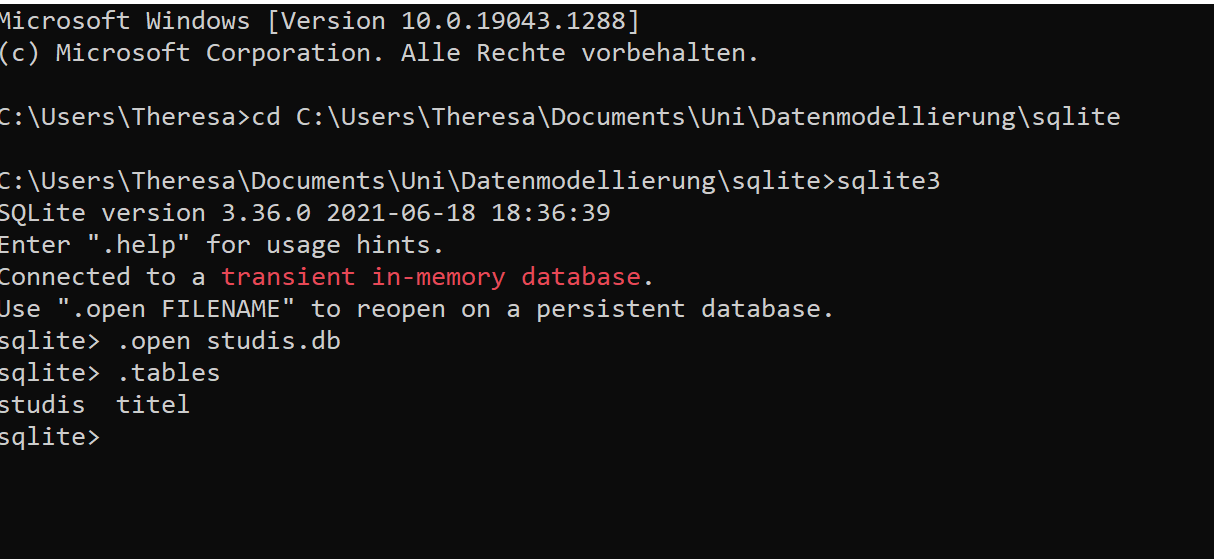
\includegraphics[width=\textwidth]{img/how_to_open_file_in_windows_sqlite3.png}

\framebreak
%---

In Sqlite3 (you can tell you're in because it says \texttt{sqlite3>} in front):
\begin{sqlcode}
.open studis.db
.tables
SELECT * FROM studis;
\end{sqlcode}
Don't forget the semicolon at the end!

Maybe before that run:
\begin{sqlcode}
.mode columns
.headers on
\end{sqlcode}

\framebreak

\begin{block}{Troubleshooting}
\begin{itemize}\small
    \item After \texttt{.open studis.db} ideally there is no output $\to$ check using \texttt{.tables} if there's any database content yet. 
    \item If there's nothing, maybe try \texttt{which sqlite3} in Mac (might not open the file you wanted but another path $\to$ navigate to correct location). 
    \item Upon clicking \texttt{sqlite3.exe } this should work under Windows but your database \texttt{studis.db} file really has to be in the same directory!
    \item Does \texttt{studis.db} seem empty? Did you open it with DB-Browser previously? This can sometimes delete the contents $\to$ re-download from Moodle and open directly via the terminal. 
\end{itemize}
\end{block}

\framebreak

\begin{block}{Potential problems}
\begin{enumerate}\small
    \item There is no data where you currently are, meaning that SQLite3 will not find anything. 
    \item You are where the data are but from there, SQLite3 cannot be accessed (maybe set environment variable or put \texttt{sqlite3.exe} into the folder). 
\end{enumerate}
\end{block}

\end{frame}

% ----------------------------------
\begin{frame}[fragile,allowframebreaks]{First SQL exercise}
\footnotesize
\metroset{block=fill}


Try these commands for the first exercise:

\begin{enumerate}
    \item First open a \texttt{.db} file as indicated above:
\begin{sqlcode}
.tables -- 2 should appear
.headers on -- maybe improve the visuals
.mode column
\end{sqlcode}

\item We create a table called \texttt{disciplines/fachgebiete}:
\begin{sqlcode}
CREATE TABLE fachgebiete (id INT, name TEXT);
.tables
\end{sqlcode}
\item $\to$ a new table should appear but it's still empty when you try the following command:
\begin{sqlcode}
SELECT * FROM fachgebiete;
\end{sqlcode}
\item  Add a new column \texttt{fachgebiet\_id}  to \texttt{studis}:  
\begin{sqlcode}
ALTER TABLE studis 
ADD COLUMN fachgebiet_id INT;
\end{sqlcode}
\item Then add both values:
\begin{sqlcode}
INSERT INTO studis (name, fachgebiet_id) 
VALUES ("Max Mara", 1);
\end{sqlcode}
or update if this row already exists (all get overwritten with value 1): 
\begin{sqlcode}
UPDATE studis SET fachgebiet_id=1;
\end{sqlcode}

\item You can put conditions $\to$ e.g.. update \texttt{studis} with \texttt{id=1} \& \texttt{id=4}, then set their discipline id to \texttt{1}:
\begin{sqlcode}
UPDATE studis SET fachgebiet_id=1 
WHERE (id = 1) AND (id = 4);
\end{sqlcode}
\item Using \texttt{.schema} I can check the setup of a table again. And save like so:
\begin{sqlcode}
.save studis_neu.db
\end{sqlcode}
\end{enumerate}

%------------------------

\begin{columns}
\column{0.5\textwidth}
$\to$ Pressing the arrow-up key gives you your last commands so you don't need to retype them each time.

$\to$ Youtube-Video to go along with the SQL basics exercise: \protect\url{https://www.youtube.com/watch?v=TpY1D13J7So} 

\column{0.43\textwidth}
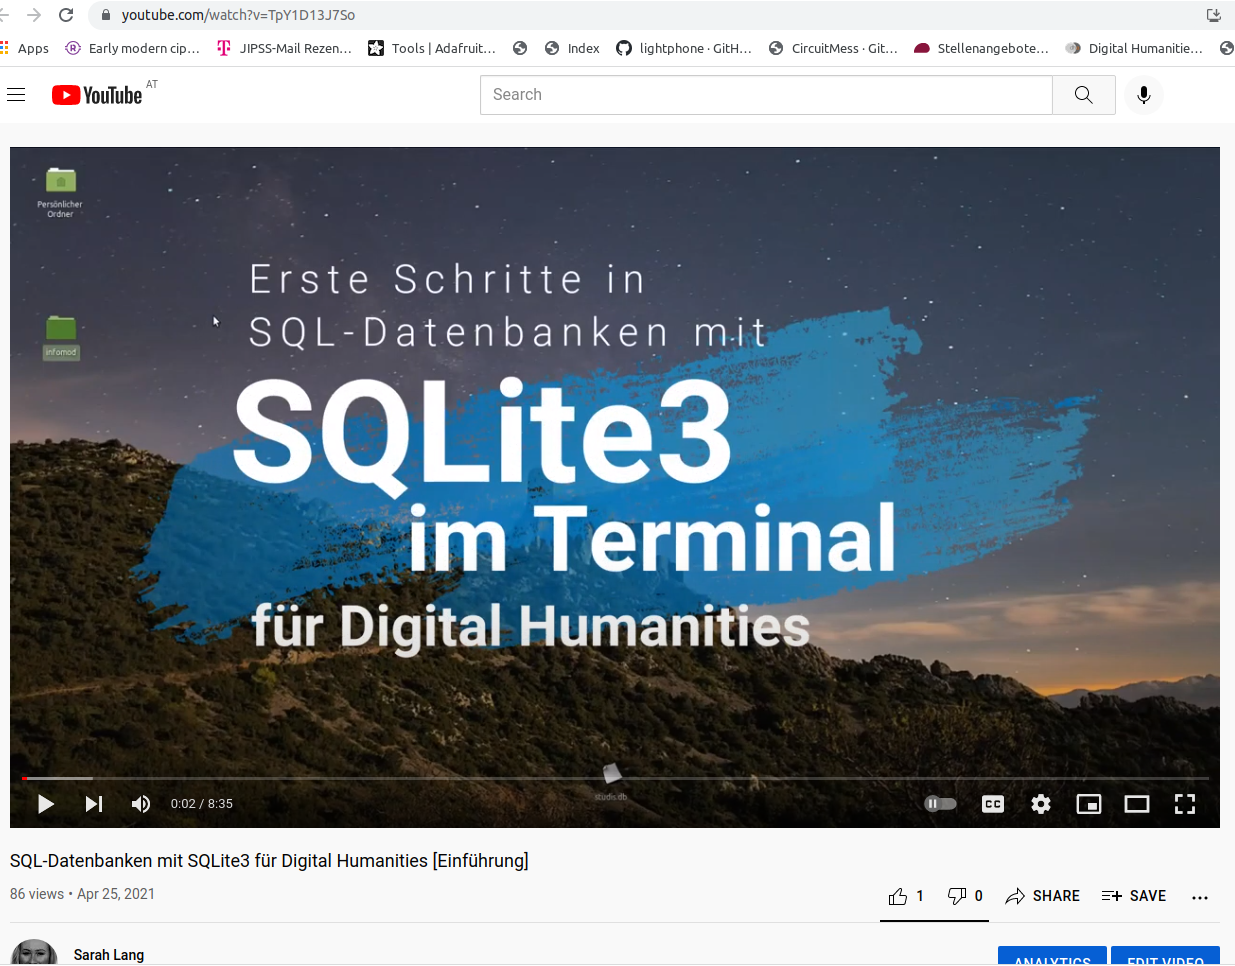
\includegraphics[width=\textwidth]{img/sql-basics-video-youtube.png}

\end{columns}

\end{frame}

%--------------------------------------------------
\begin{frame}[fragile]{CSV Import}
\small \metroset{block=fill}
    Usually you can download/export spreadsheets as \texttt{.csv}.
    You should be able to import this in SQLite3 as a table using the following command (example \texttt{city.csv} imported as a newly created table called \texttt{cities}).
\begin{sqlcode}
sqlite> .import c:/sqlite/city.csv cities
\end{sqlcode}

\begin{columns}
\column{0.48\textwidth}
Create table
\begin{sqlcode}
CREATE TABLE cities (
  name TEXT NOT NULL,
  population INTEGER NOT NULL 
);
\end{sqlcode}

\column{0.48\textwidth}
CSV Import
\begin{sqlcode}
.mode csv
.import c:/sqlite/city.csv cities
\end{sqlcode}
\end{columns}

\textbf{Tutorial:} \protect\url{https://www.sqlitetutorial.net/sqlite-import-csv/}


\end{frame}
%--------------------------------------------------

\begin{frame}[fragile]{Saving your database}
\metroset{block=fill}

    
\begin{shell-sessioncode}
oem@sary-ThinkPad-X270:~$ sqlite3
SQLite version 3.32.3 2020-06-18 14:00:33
Enter ".help" for usage hints.
Connected to a transient in-memory database.
Use ".open FILENAME" to reopen on a persistent database.
sqlite> 
\end{shell-sessioncode}


\begin{block}{Save results}
How to use \texttt{.dump} / \texttt{.save} and \texttt{.open} again
\begin{itemize}\footnotesize
    \item \protect\url{https://www.sqlitetutorial.net/sqlite-dump/}
    \item \protect\url{https://sqlite.org/cli.html}
\end{itemize}
\end{block}

\begin{sqlcode}
.save example.db
\end{sqlcode}
\protect\url{https://sqlite.org/cli.html} $\to$ under \texttt{.save}

% ----------------------------------

\end{frame}
%\section{Datenbanken}


%------------------------------------------------------------------------------
\begin{frame}{Von der Entität zur Entitätsmenge = Logisches Datenmodell Bsp. See}
  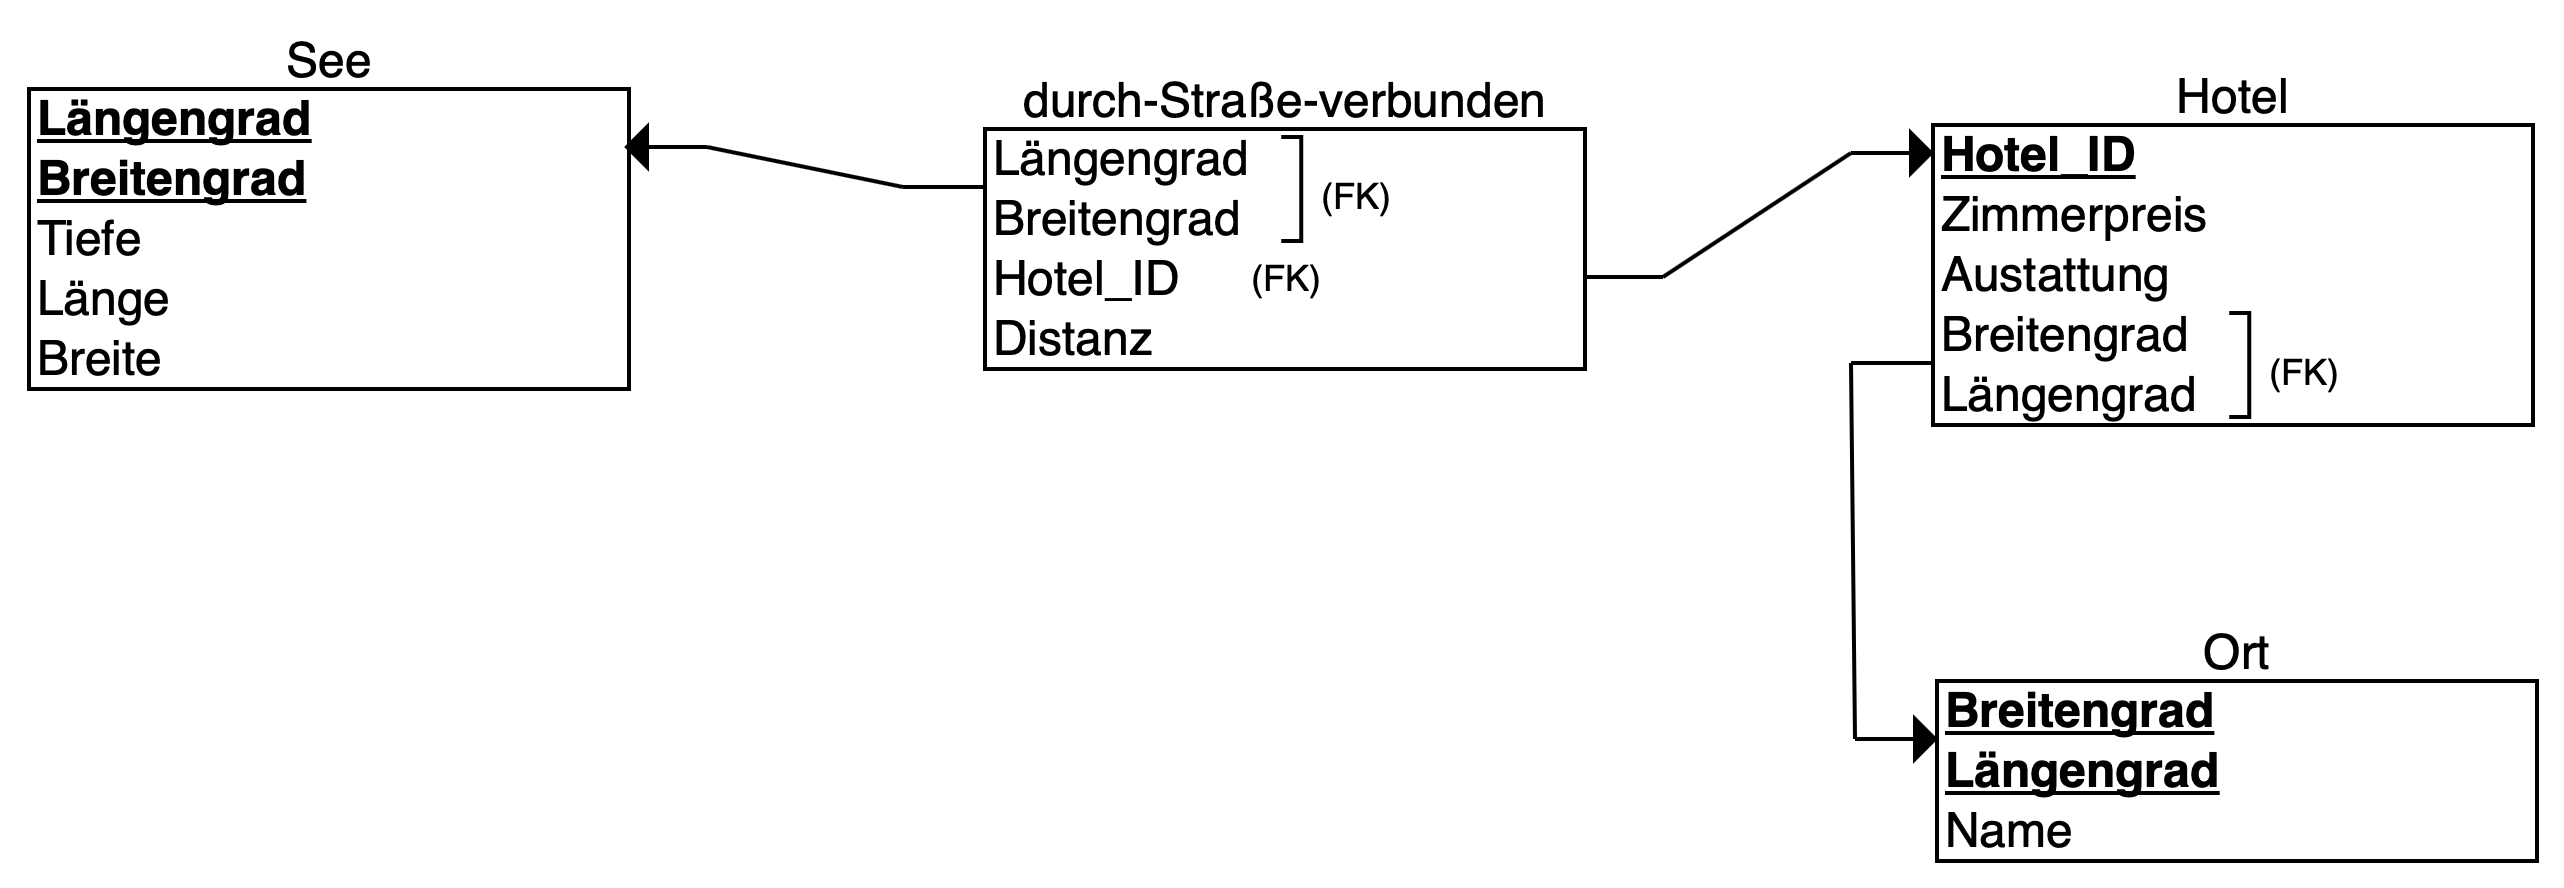
\includegraphics[width=\textwidth]{img/logisches-datenmodell-see.png} 
\end{frame}

%------------------------------------------------------------------------------
\begin{frame}{Datenbank-Schema und Beispiele}
  \metroset{block=fill}
\begin{alertblock}{1) Konzeptionelles Datenmodell}
Entity-Relationship-Diagramm
\end{alertblock}

\begin{alertblock}{2) Logisches Datenmodell }
\begin{itemize}
    \item relationales Schema
    \item hierarchisches Schema, usw.
\end{itemize}
\end{alertblock}

\begin{alertblock}{3) Physisches Datenmodell}
\begin{enumerate}
    \item \textbf{Relationale Datenbank:} SQLite, MySQL, PostgreSQL, Oracle, Microsoft SQL Server
    \item \textbf{Graphdatenbank:} Blazegraph, Neo4j
    \item \textbf{XML-Datenbank:} existdb
\end{enumerate}
\end{alertblock} 
\end{frame}

%------------------------------------------------------------------------------
\begin{frame}{Datenbank-Definitionen}
  \metroset{block=fill}
\begin{block}{Datenbasis}
Sammlung von Daten, die von einem DBMS verwaltet werden (der Datenbestand in
einem Datenbanksystem)
\end{block}

\begin{block}{Datenbankmanagementsystem (DBMS)}
Software zum Verwalten von Datenbanken
\end{block}

\begin{block}{Datenbanksystem}
Ein Datenbankmanagementsystem und die von ihm verwalteten Daten. \\
Umgangssprachlich ist oft das mit dem Begriff `Datenbank' gemeint.
\end{block}

\end{frame}


%------------------------------------------------------------------------------
\begin{frame}[allowframebreaks]{DBMS}
  \metroset{block=fill}
\begin{alertblock}{Was ist ein Datenbankmanagementsystem (DBMS)?}
Ein Datenbankmanagementsystem ist eine Software zum Betrieb von
Datenbanksystemen, also zur Verwaltung von Datenbasen
\end{alertblock}

\begin{exampleblock}{Basisfunktionalität}
\begin{enumerate}
    \item Definition von Datenstrukturen (via Data Definition Language)
    \item Manipulation von Daten (Einfügen, Ändern, Löschen) (via Data Manipulation Language)
    \item Abfrage  eines Datenausschnitts (via Query Language)
    \item Dauerhafte Speicherung der Daten (nicht zwingend bei jeder DB)
\end{enumerate}
\end{exampleblock}


\end{frame}


%------------------------------------------------------------------------------
\begin{frame}{Historische Datenbankmodelle}
Quelle: DB-LV Slides (Gunter Vasold)
  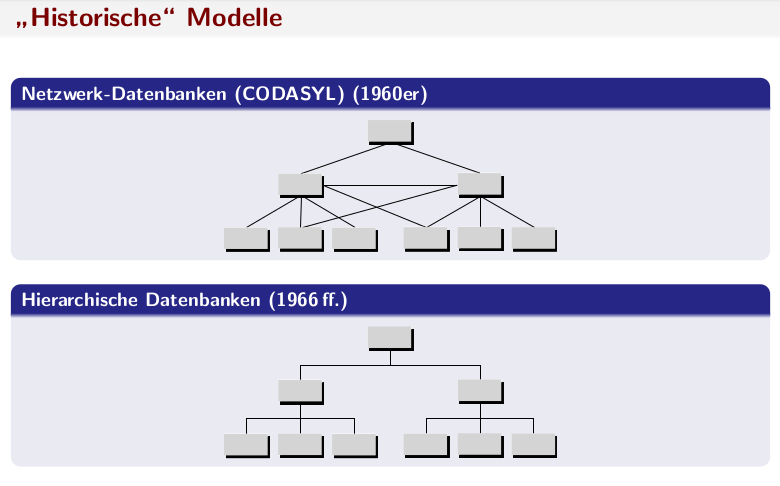
\includegraphics[width=\textwidth]{img/gunther-histor-db-modelle.png}
\end{frame}


%------------------------------------------------------------------------------
\begin{frame}{Relationale Datenbankmodelle}
Quelle: DB-LV Slides (Gunter Vasold)
  \includegraphics[width=\textwidth]{img/gunter-rel-db.png}
\end{frame}


%------------------------------------------------------------------------------
\begin{frame}{Datenbankmodelle: Historische Entwicklung}
\begin{enumerate}
    \item Objektorientierte Datenbanken (v.a. 1990er-Jahre)
    \item Objektrelationale Datenbanken (1990er-Jahre ff.)
    \item NoSQL-Datenbanken (2000er-Jahre f.)
    \item XML-Datenbanken
    \item Document Stores
    \item Wide Column Stores
    \item Key-Value Stores
    \item Graphenbasierte Datenbanken
\end{enumerate}
\end{frame}


%------------------------------------------------------------------------------
\begin{frame}[standout]
    \alert{Lektüre}-Zusammenfassung: \\
    McCarty, Modelling \\[1em]
    {\footnotesize Bitte \alert{\href{https://docs.google.com/presentation/d/1v_j9Jms21hZokX9hLJ_7kcnV63FJPHTHNowfLVLiYys/edit?usp=sharing}{hier im Google Slides zusammenfassen}}; 1 Person stellt dann vor. \\
    }
\end{frame}


%------------------------------------------------------------------------------
\begin{frame}[standout]
    \alert{Übung:} \\ \small Erklären Sie Ihren Gruppenteilnehmern, welche Entitätstypen in Ihrem Original vorkommen. \\
    Erklären Sie Ihren Gruppenteilnehmern, welchen Zweck ein Filtern und Sortieren der Entitäten für den Modellbenutzer haben könnte.
\end{frame}

 %TODO - wasnt done in this class


\section{SQL}

\begin{frame}[fragile,allowframebreaks]{Structured Query Language (SQL)}
  \metroset{block=fill}
\begin{block}{Database functions}
\begin{itemize}
    \item \textbf{SQL:} \emph{standardized} query language for relational databases
    \item \textbf{Data Definition Language (DDL):} create database
    \item \textbf{Data Manipulation Language (DML):} query and modify data 
    \item \textbf{Data Storage Description Language (DSDL):} write data on physical storage structure
\end{itemize}
\end{block}

\begin{exampleblock}{Ressources/Tutorials}
\begin{itemize}\footnotesize
    \item  \textbf{SQL:} \protect\url{ https://www.w3schools.com/sql/ }
    \item  \textbf{SQLite:} \protect\url{https://www.sqlitetutorial.net }
    \item \protect\url{https://sqlite.org/cli.html}
\end{itemize}
\end{exampleblock}


\begin{alertblock}{Good to know}
\mycommand{*}{sog. \emph{Wildcard}, matches/means: everything}
\mycommand{;}{expected as an end marker for SQL statements (not just ENTER)}
\end{alertblock}


\begin{alertblock}{\texttt{.dot} commands versus \texttt{;}}
\footnotesize
Using \texttt{.} tells the software to use an internal command from a fixed set of commands and not wait for \texttt{;} $\to$ only works for this predetermined set of commands!
\end{alertblock}

\begin{alertblock}{Open SQLite-shell (SQL commands)}
\mycommand{.shell cd directory }{change directory}
\mycommand{.save dbname }{save database}
\mycommand{.open dbname }{open previously saved db}
\end{alertblock}

\begin{exampleblock}{Using SQL}
\begin{enumerate}
    \item via the \alert{Terminal} (=commandline); in Windows \texttt{cmd} (search for it) $\to$ click \texttt{sqlite3.exe} or type \texttt{sqlite3}: 
    \begin{itemize}
        \item if there is no error, it's working and waiting for prompts!
        \item more info on SQLite CLI: \protect\url{https://sqlite.org/cli.html}
    \end{itemize}
    \item via \alert{SQLiteBrowser} (not recommended)
    \item possible \alert{file endings} to import: \texttt{.csv}, \texttt{.db}, \texttt{.sql}
\end{enumerate}
\end{exampleblock}


\begin{alertblock}{Special commands to sqlite3 (dot commands)}
 \mycommand{.help}{overview over dot commands}
\mycommand{.open ?OPTIONS? ?FILE? }{open or create db}
\mycommand{.databases }{show existing dbs}
\mycommand{.tables ?TABLE? }{show existing tables}
\mycommand{.import FILE TABLE }{import data to table}
\mycommand{.mode MODE ?TABLE? }{how to display output}
\mycommand{.mode column}{show \texttt{SELECT} results as tabular format}
\mycommand{.headers on}{show \texttt{SELECT} results with headers}
\mycommand{.schema ?TABLE? }{displays \texttt{CREATE} command used}
\mycommand{.save ?FILE? }{save the db}
\mycommand{.dump ?TABLE?}{show database contents as SQL commands}
\end{alertblock}

\end{frame}


%------------------------------------------------------------------------------
\begin{frame}[fragile]{Tutorial: Beginner SQL using SQLiteBrowser or Terminal}
\small
%oder einfach:
\begin{verbatim}
    > sqlite3 studis.db
\end{verbatim}
 
\begin{columns}
\column{0.45\textwidth}
\includegraphics[width=0.8\textwidth]{img/youtube-sqlitebrowser.png}

ca. 10min Video \\
\protect\url{https://www.youtube.com/watch?v=Pni6WxHFTUg} \\

\column{0.45\textwidth}
\includegraphics[width=0.8\textwidth]{img/sql-basics-video-youtube.png}

ca. 8min \\
\protect\url{https://www.youtube.com/watch?v=TpY1D13J7So&t=413s} \\

\end{columns}
\end{frame}


%------------------------------------------------------------------------------
\begin{frame}[fragile]{Some more SQL}
  \metroset{block=fill}
  \begin{columns}[T,onlytextwidth]
    \column{0.4\textwidth}
    
      \begin{block}{selection criteria}
        \begin{itemize}\footnotesize
            \item %Testausdruck: Feldname Operator Wert; Operator kann sein z.B. 
            Use operators like \texttt{=, !=, >, <, LIKE, REGEX, MATCH, ISNULL, NOTNULL}
            \item %Verknüpfung von mehreren Testausdrücken mit 
            Combine using \texttt{AND} or \texttt{OR}
        \end{itemize}
      \end{block}
      
    \column{0.55\textwidth}
\begin{block}{Print results}
\begin{sqlcode}
SELECT content 
FROM Tabelle 
WHERE selectionCriteriaMatch
\end{sqlcode}
\end{block}

\begin{block}{Reduce set of results}
  \begin{sqlcode}
SELECT content 
FROM Tabelle 
WHERE selectionCriteriaMatch
LIMIT max number of results
OFFSET results starting from...
\end{sqlcode}
\end{block}

  \end{columns}
\end{frame}


%------------------------------------------------------------------------------
\begin{frame}[fragile]{Delete or modify tables (DDL)}

\begin{block}{Delete table }
  \begin{sqlcode}
  DROP TABLE tableName;
  \end{sqlcode}
\end{block}

\begin{block}{Rename table }
  \begin{sqlcode}
  ALTER TABLE tableName RENAME TO tableName;
  \end{sqlcode}
\end{block}

\begin{block}{Add column}
  \begin{sqlcode}
  ALTER TABLE tableName 
  ADD COLUMN columnname1 datatype options;
  \end{sqlcode}
\end{block}
\end{frame}

%------------------------------------------------------------------------------
\begin{frame}[fragile]{Insert data = data representation (DML)}

\begin{block}{Add new row}
  \begin{sqlcode}
INSERT INTO tableName 
       (columnname1, columnname2, columnname3 [etc.]) 
       VALUES (value1, value2, value3 [etc.]);
\end{sqlcode}
\end{block}

\begin{block}{add multiple rows at a time}
  \begin{sqlcode}
VALUES (value1, value2, value3 [etc.]), 
       (value1, value2, value3 [etc.]), 
       (value1, value2, value3 [etc.]) [etc.]; 
\end{sqlcode}
\end{block}

\end{frame}


%------------------------------------------------------------------------------
\begin{frame}[fragile, allowframebreaks]{Example: delete or change entries (DML) }
\begin{block}{Change entries}
    \begin{sqlcode}
UPDATE tableName 
SET columnname_to_modify = new_value
WHERE columnname = referenceValue;
\end{sqlcode}
\end{block}

\begin{block}{Delete entries}
  \begin{sqlcode}
DELETE FROM tableName 
WHERE columnname = value;
\end{sqlcode}
\end{block}

\framebreak

\begin{block}{Query the db (DML) }
  \begin{sqlcode}
SELECT * FROM tableName;
SELECT table1, table3 FROM tableName;
\end{sqlcode}
\end{block}

\framebreak

German video slowly showing all steps from the first basic example: 

\includegraphics[width=0.65\textwidth]{img/sql-basics-video-youtube.png}

\framebreak

Our example from the intro.

\begin{columns}
\column{0.42\textwidth}
\begin{sqlcode}
.tables

ALTER TABLE studis
ADD COLUMN fachgebiet_id INT;

CREATE TABLE fachgebiet (
name TEXT,
id INT PRIMARY KEY
);

.tables
\end{sqlcode}

\column{0.58\textwidth}
\begin{sqlcode}
INSERT INTO fachgebiet (name, id)
VALUES ('dh', 1), ('geschichte', 2);

UPDATE studis 
SET fachgebiet = 2
WHERE id = 1;

SELECT * FROM studis;

SELECT name, fachgebiet 
FROM studis;
\end{sqlcode}
\end{columns}

\end{frame}

% Erstellen Sie mind. eine Entitätenmenge oder Beziehungsmenge (Tabelle) Ihres Originals mithilfe von SQL in der Kommandozeile. Laden Sie die Datenbank (.db) auf Moodle hoch.


%------------------------------------------------------------------------------
\begin{frame}[standout]
    What can you do with \alert{\texttt{urlaub.db}}?
\end{frame}

%------------------------------------------------------------------------------
\begin{frame}[standout]
    \alert{Homework 4: } Get started creating your database! \\[0.5em]
    \small Create a project database for your final project in SQL. 
    Write 1/2-1 page of text (submitted as PDF) explaining the following questions:
    {\footnotesize 
    \begin{itemize}
        \item  Which original are you modelling?
        \item What is the purpose of the database? Which queries do you want to answer with it?
        \item Which entities of the original are represented in your database?
        \item Which attributes (incl. Primary Keys) do the classes have?
\end{itemize}
    }
    Also submit a dump of your database please.
\end{frame}

%------------------------------------------------------------------------------
\begin{frame}[fragile]{SQL basics}
\begin{columns}
  \column{0.6\textwidth}
  \begin{enumerate}\footnotesize
      \item Our terminal expects that all statements are terminated by \texttt{;} -- this allows you to use line breaks to structure your query for better overview. If you forget the semicolon the terminal will keep waiting for input. It might look like it's stuck: Just type semicolon plus enter to fix it. 
      \item Asterisk (\texttt{*}) is a so-called \emph{wildcard} and means `everything'.
      \item Our simple first statement thus means: `Select \emph{everything} from the table named \emph{table}.'
      \item You can open databases (\texttt{.db} or \texttt{.sql}) using \texttt{sqlite3 databasename.db} from the terminal.
  \end{enumerate}
  \column{0.35\textwidth}
    \metroset{block=fill}
    \begin{block}{My first SQL statement}
    \footnotesize
    Before running your first command, you might need to use the \texttt{.tables} command in \texttt{sqlite3} to learn which tables even exist in your database and/or how they are named  (dot-prefixed commands exceptionally need no semicolon to end them, just enter).
    \begin{sqlcode}
    SELECT * FROM table;
    \end{sqlcode}
\end{block}

\end{columns}
\end{frame}


%------------------------------------------------------------------------------
\begin{frame}[fragile]{SQL basics 2}
\begin{columns}
  \column{0.6\textwidth}
  \begin{enumerate}\footnotesize
      \item If there was a mistake in your command, you get an error message. If there is none we assume all is good and whatever you prompted the program to do actually happened. There might just not be a success message. But what you prompted the program to do might not have been exactly what you had \emph{intended} it to do, so inspect the results by displaying your database anew!
      \item After you change a database, check its contents using  \texttt{SELECT * FROM table;} $\to$ make sure the change effected was the one intended.
      \item By convention, SQL keywords are capitalized in AllCaps style to make them easily identifiable visually. This makes your code more readable but the program would also work with lowercase commands.
  \end{enumerate}
  \column{0.45\textwidth}
More complex example:
  \begin{sqlcode}
SELECT DISTINCT column_list
FROM table_list
JOIN table ON join_condition
WHERE row_filter
ORDER BY column
LIMIT count OFFSET offset
GROUP BY column
HAVING group_filter;
\end{sqlcode}
\end{columns}
\end{frame}


%------------------------------------------------------------------------------
\begin{frame}[fragile, allowframebreaks]{SQL SELECT}
\begin{sqlcode}
SELECT list_of_columns FROM list_of_tables;
\end{sqlcode}
\begin{exampleblock}{What the options mean\dots}
\begin{description}\footnotesize
  \item[list\_of\_columns] you can select multiple columns separated by comma or use asterisk (\texttt{*}) to select all
  \item[list\_of\_tables] defines which tables to select from. 
  \item[AS (alias)] allows you to name the column header for the output table
  \item[DISTINCT] only prints each unique value once; \textbf{usage:} \texttt{SELECT DISTINCT}
\end{description}
\end{exampleblock}

\framebreak
\small 
To select specific columns from multiple tables which share common column names, specify as follows:
\begin{sqlcode}
SELECT hotels.name, places.name FROM hotels, places;
\end{sqlcode}
For more clarity, give them more meaningful headers:
\begin{sqlcode}
SELECT hotels.name AS hotel_name, 
       places.name AS place_name 
FROM hotels, places;
\end{sqlcode}
Not specifying from which table will either print a cartesian product or produce an error like so:
\begin{sqlcode}
SELECT name FROM hotel, place;
-- Error: ambiguous column name: name
\end{sqlcode}
  %\includegraphics[width=\textwidth]{img/select-ueberblick.png} 

\end{frame}


%------------------------------------------------------------------------------
\begin{frame}[fragile]{SQL WHERE}
\small 
Entries are selected depending on the values of their attributes which are communicated using the following operators:
\begin{columns}
  \column{0.33\textwidth}
  \begin{block}{Comparison operators}
    \begin{description}\footnotesize
      \item[=] equals
      \item[>] greater than
      \item[<] less than
      \item[>=] greater or equal
      \item[<=] less or equal
      \item[!= or <>] not equal
    \end{description}
  \end{block}

  \column{0.66\textwidth}
  \begin{block}{Logical operators}\footnotesize
    \begin{description}
      \item[AND] both are true
      \item[OR] at least one part is true
      \item[BETWEEN] value is within a defined range
      \item[IN] value in included in defined set
      \item[LIKE] value corresponds to a pattern
      \begin{description}
        \item[\%] any sequence of characters (none or multiple)
        \item[\_] any one character (exactly one)
      \end{description}
      \item[NOT] results in the opposite of the truth value of the expression
    \end{description}
  \end{block}
\end{columns}
\begin{sqlcode}
SELECT name FROM hotel WHERE price < 150;
\end{sqlcode}
  %\includegraphics[width=\textwidth]{img/sql-where.png}  
\end{frame}

%------------------------------------------------------------------------------
\begin{frame}[fragile, allowframebreaks]{SQL CREATE VIEW}

  If you need to rearrange the order of your table after it is already defined or just getting an output that you often need is very complicated and annoying, you might want to create a \texttt{VIEW} so that you can access the result of a complex query over and over again effortlessly:
  \begin{sqlcode}
CREATE VIEW view_name AS
SELECT column1, column2, ...
FROM table_name
WHERE condition; 
  \end{sqlcode}
  It will always show up-to-date data as it's just a shorthand for the actual complex query. 
  \framebreak
  
  \href{https://www.w3schools.com/sql/sql_view.asp}{W3C Tutorial 'CREATE VIEW'} $\to$ \textbf{examples:}
        \begin{sqlcode}
CREATE VIEW [Brazil Customers] AS
SELECT CustomerName, ContactName
FROM Customers
WHERE Country = 'Brazil';

-- display as:
SELECT * FROM [Brazil Customers]; 
  \end{sqlcode}

        \begin{sqlcode}
CREATE VIEW [Products Above Average Price] AS
SELECT ProductName, Price
FROM Products
WHERE Price > (SELECT AVG(Price) FROM Products); 
-- call as:
SELECT * FROM [Products Above Average Price]; 
  \end{sqlcode}


\end{frame}


%------------------------------------------------------------------------------
\begin{frame}[fragile]{Creating tables (DDL)}
\begin{sqlcode}
CREATE TABLE tableName (
  columnName1 datatype option,
  columnName2 datatype option,
  [...]
  );
\end{sqlcode}
\begin{exampleblock}{What the options mean\dots}
\begin{description}\footnotesize
  \item[tableName] represents the entity set, written in lowercase.
  \item[columnName] represents an attribute or relationship of the entity, in lowercase. 
  \item[datatype] sets the data type from a list of possibilities such as \texttt{TEXT} or \texttt{INTEGER}, etc.
  \item[options] 
  \begin{itemize}
      \item \textbf{Primary Key:} \texttt{PRIMARY KEY} $\to$ sets value as primary key.
      \item \textbf{Foreign Key:} \texttt{FOREIGN KEY columnName REFERENCES tableName\_pk(attribute\_pk)} $\to$ sets value as foreign key.
      \item \textbf{No empty values allowed:} \texttt{NOT NULL}.
      \item \textbf{Values have to be unique:} \texttt{UNIQUE}.
  \end{itemize}
\end{description}
\end{exampleblock}
 % \includegraphics[width=\textwidth]{img/tabellen-erstellen-ddl.png}
\end{frame}



%------------------------------------------------------------------------------

\section{Database organization, Primary and Foreign Keys}
%------------------------------------------------------------------------------
\begin{frame}[fragile]{Data types}
  \metroset{block=fill}\footnotesize
      \begin{alertblock}{Data types}
        \begin{itemize}
            \item \textbf{NULL} nothing
            \item \textbf{INTEGER} positive integer values (Ganzzahlen)
            \item \textbf{REAL} 8-byte IEEE floating point values
            \item \textbf{TEXT} text encoded according to DB standard (UTF-8, UTF-16BE or UTF-16LE).
            \item \textbf{BLOB} The value is a blob of data, stored exactly as it was input.
        \end{itemize}
      \end{alertblock}
      
      Other database management systems (DBMS) have a slightly different choice of datatypes due to different implementations. \textbf{Remember: }SQL is a standard which is implemented slightly differently by different software solutions such as \texttt{SQLite3} or \texttt{MySQL} (\alert{\href{https://www.w3schools.com/sql/sql_datatypes.asp}{check out this list}}).
      
      In MySQL, instead of \texttt{TEXT} you would use this:
      \begin{sqlcode}
          LastName varchar(255),
      \end{sqlcode}
      This tells the computer exactly for how many characters it needs to reserve space. This used to be more important especially when computer memory was more rare a commodity than it is today.  
      
\end{frame}


%------------



%------------------------------------------------------------------------------
\begin{frame}[allowframebreaks]{Primary and Foreign Keys}
    % ----------------------------------------------
{\scriptsize Source: Gunter Vasold, \emph{Datenbanken} class (summer term 2017)}
\metroset{block=fill}

      \begin{block}{}
      \centering \includegraphics[width=0.48\textwidth]{img/autor-id-titel.png}~\includegraphics[width=0.48\textwidth]{img/foreign-key.png}
      \end{block}

\begin{itemize}\scriptsize
\item Because relations are sets, each tuple needs to be different from all others. To address one specific tuple, we need a key or an id. This key needs to be unique in the whole relationship set. 
\item A key (\emph{primary key}, \textbf{Primärschlüssel}) can consist of one or multiple attributes (as few as possible, it has to be irreducible or minimal). In practice, we often use artificial keys (like a running id number). 
\item \textbf{Foreign keys} (\emph{Fremdschlüssel}) reference the primary key of a tuple in a different relation. Because foreign keys don't need to be unique, they aren't technically keys but are still called that way. Comparing foreign and primary keys, we can create new relations ad hoc.
\end{itemize} 
    %\begin{block}{}\centering\includegraphics[width=0.9\textwidth]{img/foreign-keys-studyflix.png}\end{block} % https://studyflix.de/informatik/relationale-datenbanken-600

\framebreak

\includegraphics[width=0.9\textwidth]{img/foreign-keys-linked.png}\bigskip

\metroset{block=fill}  
      \begin{exampleblock}{Referential integrity}\footnotesize
Referential integrity is a constraint which ensures that a dataset can only be manipulated if it doesn't render other datasets inconsistent. 

\textbf{Example:} Deleting dataset with \texttt{id=4} in the table \texttt{author} would destroy referential integrity because at least one foreign key in the table \emph{book} references this entry. For the machine to automatically know that, we need to declare these keys and their relationships when setting up the database (more on that later).
      \end{exampleblock}
\end{frame}
%------------------------------------------------------------------------------
\begin{frame}[fragile, allowframebreaks]{Unique Identifiers: Primary and Foreign Keys}
  \metroset{block=fill}
\begin{exampleblock}{Identifier}
\textbf{unique identifier / key:} refers to exactly one element. Examples: \vspace{-1em}
      \begin{enumerate}
          \item ISBN no.
          \item matriculum nr.
          \item ORCID-ID
          \item DOI
          \item car plate
          \item norm data (GND): list of standardized terminoloy, gives a definite name form and an ID to refer to
      \end{enumerate}
      \end{exampleblock}
      
\begin{exampleblock}{Indirection} An ID doesn't directly point to a value but rather to a number which, in turn, points to the value. 
\end{exampleblock}

\begin{exampleblock}{Separating contents into multiple tables minimizes redundancy!}  
Data can be reunited (joined) using \texttt{VIEW}s. Redundancy is a source of errors.
\end{exampleblock}
\framebreak 

Each table needs to have its primary key. You can define it in the two following ways:
\begin{enumerate}\small 
    \item as an added option when defining the column:
\begin{sqlcode}
id INT PRIMARY KEY
\end{sqlcode}
    \item as an extra option after all column definitions:
\begin{sqlcode}
PRIMARY KEY(id)
PRIMARY KEY(forname, lastname, birthday)
\end{sqlcode}
\end{enumerate}

\begin{alertblock}{Resources}
  \begin{enumerate}\footnotesize
      \item \href{https://www.w3schools.com/sql/sql_primarykey.asp}{W3Schools Primary Key}: unique identifier for each table entry
      \item \href{https://www.w3schools.com/sql/sql_unique.asp}{W3Schools UNIQUE}
      \item \href{https://www.w3schools.com/sql/sql_notnull.asp}{W3Schools NOT NULL}
  \end{enumerate}
\end{alertblock}

\end{frame}

%------------------------------------------------------------------------------
\begin{frame}[fragile]{Linking tables}
  \metroset{block=fill}
  Example: Linking tables using keys \bigskip 
\small 
\begin{columns}
  \column{0.3\textwidth}
    \begin{block}{}
        \begin{enumerate}
            \item \textbf{Class:} \underline{ClassID}, LecturerID, subject, RoomID, hours
            \item \textbf{Room:} \underline{RoomID}, building, capacity
            \item \textbf{Lecturer:} \underline{LecturerID}, name, area of expertise
            \item \textbf{Student:} \underline{StudentID}, name, area of study
        \end{enumerate}
      \end{block}
  \column{0.72\textwidth}
Generic example:
\begin{sqlcode}
CREATE TABLE person (
   id      INTEGER PRIMARY KEY AUTOINCREMENT,
   name    TEXT   NOT NULL,
   age     INT    NOT NULL,
   address TEXT
);
\end{sqlcode}

Class example:
\begin{sqlcode}
CREATE TABLE student (
   student_id      INTEGER PRIMARY KEY,
   name            TEXT    NOT NULL,
   degreeProgramme TEXT    NOT NULL
);
\end{sqlcode}
\end{columns}
\end{frame}


%------------------------------------------------------------------------------
\begin{frame}[fragile, allowframebreaks]{Using Foreign Keys join tables}
\metroset{block=fill}
\footnotesize

Each table only contains one type of entity (e.g. student's names and ID numbers). But these might have relationships to other tables, for example, for each student we could list course numbers. Using this course number we get a link to a course table where we write down the name of the class.


\begin{alertblock}{Foreign Keys (\emph{Fremdschlüssel})}
\footnotesize
It is not mandatory to specify Foreign Keys but they allow the database to run internal optimization in the background. They are essential for maintaining referential integrity. 

You can define them as follows:
\begin{enumerate}
    \item as part of the respective column definition:
\begin{sqlcode}
REFERENCES tableNname(fieldName)
\end{sqlcode}
    \item after the column definitions:
\begin{sqlcode}
FOREIGN KEY(columnName) REFERENCES tablenName(fieldName)
\end{sqlcode}
\end{enumerate}
\end{alertblock}

\framebreak 
Assuming there were another table called \texttt{places}
with the primary key \texttt{id}
\begin{sqlcode}
CREATE TABLE persons (
  place_id INT UNSIGNED REFERENCES places(id),
  ...
);

CREATE TABLE persons (
  place_id INT UNSIGNED ,
  ...
  FOREIGN KEY (place_id) REFERENCES places(id)
);
\end{sqlcode}
\framebreak 

This \emph{Foreign Key} refers to another table's \emph{Primary Key}. 
Assuming there is a \texttt{disciplineID} in the \texttt{disciplines} table where it is the\emph{Primary Key}. 
In the \texttt{Students} table would be a column called \texttt{disciplineID} which is a foreign key \emph{Foreign Key there.}


\begin{block}{Foreign Key constraints in \texttt{CREATE TABLE}}
\begin{sqlcode}
FOREIGN KEY (columnName) 
REFERENCES tableName_pk (attribute_pk)
PRAGMA foreign_keys = ON;
\end{sqlcode}
\end{block}

Using \texttt{FOREIGN KEY} constraints we could define what happens if, for example, one of the related tables gets updated or something is deleted. 
\end{frame}

%------------------------------------------------------------------------------
\begin{frame}[fragile, allowframebreaks]{Constraints}
\metroset{block=fill}
\footnotesize

\begin{alertblock}{\href{https://www.w3schools.com/sql/sql_constraints.asp}{W3Schools SQL Constraints}}
  \begin{description}\footnotesize 
      \item[NOT NULL] makes sure a field can never be \texttt{NULL} (important for IDs). 
      \item[UNIQUE] makes sure all values of a column are distinct (also important so that IDs remain unique). 
      \item[PRIMARY KEY] automatically creates a combination of \texttt{NOT NULL} and \texttt{UNIQUE}, making the primary key an ideal means of referencing a table entry. 
      \item[FOREIGN KEY] prevents relationships between tables from accidentally getting destroyed (by the deletion of a cell, for example, to which the cells of another table still refer).
      \item[CHECK] makes sure the values of a column correspond to certain constraints (such as age is in between 0-99 or similar). This prevents you from accidentally inserting nonsensical values into the table which could later corrupt any analyses you might want to use the database for. 
  \end{description}
\end{alertblock}


\begin{alertblock}{Value constraints}
  Many DBMSs allow you to define any allowed range for value for a given column. Syntax:
\begin{sqlcode}
CHECK ([ fieldname ] [ condition ])
\end{sqlcode}

Example
\begin{sqlcode}
CREATE TABLE teachers (
salary DECIMAL (4 ,2) ,
CHECK ( salary > 0)
)
...
CHECK (grade >0 AND grade <=5)
\end{sqlcode}
\end{alertblock}

\end{frame}





%------------------------------------------------------------------------------
\begin{frame}{Excursus: SQL Injection (definition)}
  \metroset{block=fill}

  \begin{columns}
    \column{0.48\textwidth}
\begin{alertblock}{\href{https://en.wikipedia.org/wiki/SQL_injection}{Wikipedia}}\footnotesize
SQL injection is a code injection technique used to attack data-driven applications, in which malicious SQL statements are inserted into an entry field for execution (e.g. to dump the database contents to the attacker).
\end{alertblock}
\bigskip

\begin{block}{related \texttt{xkcd} comic} 
\includegraphics[width=0.95\textwidth]{img/exploits_of_a_mom.png}
\scriptsize
\href{https://xkcd.com/327/}{source}
\end{block}

\column{0.48\textwidth}
\begin{exampleblock}{\href{https://www.w3schools.com/sql/sql_injection.asp}{W3Schools}}\footnotesize
SQL injection is one of the most common web hacking techniques. 

SQL injection is the placement of malicious code in SQL statements, via web page input.

SQL injection usually occurs when you ask a user for input, like their username/userid, and instead of a name/id, the user gives you an SQL statement that you will \textbf{unknowingly} run on your database.
\end{exampleblock}
\end{columns}
\end{frame}

%------------------------------------------------------------------------------
\begin{frame}[fragile]{Excursus: SQL Injection (example from W3Schools)}
  \metroset{block=fill}

    \begin{block}{Starting point}
    \scriptsize
    A website gets data using a form to later run a database query whose results are to be displayed to the user. Example in javascript:
  \begin{jscode}
txtUserId = getRequestString("UserId");
txtSQL = "SELECT * FROM Users WHERE UserId ="
         + txtUserId;
  \end{jscode}
\end{block}

  \begin{columns}
    \column{0.48\textwidth}
\begin{block}{Always True Inject}\scriptsize
In case there are no security checks when parsing the submitted query, users can submit SQL code instead of just a normal value. 
\texttt{OR 1=1} is always true, thus all users will be displayed. Resulting SQL query (obviously it was not intended by the database owners to use the form like this):
  \begin{sqlcode}
  SELECT * FROM Users 
  WHERE UserId = 105 OR 1=1;
  \end{sqlcode}
\end{block}
\column{0.48\textwidth}
\begin{block}{Batched Statement Inject}\scriptsize
Instead of just running one statement, one could also add \texttt{;} and send a second query after it. For example by typing into the form: \texttt{105; DROP TABLE Users}. Resulting SQL code: 
  \begin{sqlcode}
  SELECT * FROM Users 
  WHERE UserId = 105; 
  DROP TABLE Users;
  \end{sqlcode}
\end{block}
  \end{columns}
\end{frame}



%------------------------------------------------------------------------------


\begin{frame}[fragile, allowframebreaks]{Cardinality}
\metroset{block=fill}

\begin{alertblock}{Cardinality}\small
Cardinality describes how many entities participate in a relationship. The following cardinalities are possible:
  \begin{description}\footnotesize
      \item[1:1] exactly one-to-one relationship, quite rare in practice.  \\\textbf{\scriptsize Example:} \emph{\scriptsize Student can only have one passport photo.}
      \item[1:n] (directionality can also be n:1 !) Exactly one entity is linked to one or multiple others.  \\\textbf{\scriptsize Example:} \emph{\scriptsize Student can have multiple adresses.}
      \item[n:m] Both parts of the relationship can participate in multiple relationships. \\\textbf{\scriptsize Example:} \emph{\scriptsize Students can go to multiple classes; most classes should have more than one student.}
  \end{description}
\end{alertblock}

\end{frame}

%------------------------------------------------------------------------------
\begin{frame}{Remember: How to represent entities in a database}
    \begin{itemize}
        \item \textbf{entity} $\to$ table
        \item \textbf{attribute} $\to$ column
        \begin{itemize}
            \item multi-valued attributed $\to$ helper table
        \end{itemize}
        \item \textbf{relationship}
            \begin{itemize}\footnotesize
                \item \textbf{1:1} $\to$ Key of one entity (table) is stored as reference (`foreign key'/`Fremdschlüssel') in the other table as a column/attribute of its own 
                \item \textbf{1:n} $\to$ key of the 1-ary entity/table stored as reference in the n-ary table/entity 
                \item \textbf{n:m} $\to$ table of its own containing the keys of both related entities
                \item \textbf{n-ary relations} $\to$ helper table containing the keys of all entities as columns 
                \item \textbf{relationship attributes} $\to$ helper table with the keys of participating entities and columns for the attributes 
                \item \textbf{multi-valued attributes} $\to$ helper table with entity key as foreign key (like a 1:n relation) and a column for the attribute 
                \item \textbf{composite attributes} $\to$ helper table with entity key as foreign key (like a 1:n relation) and columns for the partial attributes 
            \end{itemize}
    \end{itemize}
\end{frame}
  
\section{More advanced queries}
%------------------------------------------------------------------------------
\begin{frame}[fragile, allowframebreaks]{Functions, sorting, counting, etc.}
%\metroset{block=fill}

\begin{columns}
\column{0.44\textwidth}
\begin{block}{COUNT}
  \begin{sqlcode}
SELECT COUNT(columnname) 
FROM tablenname 
WHERE bedingung ;
\end{sqlcode}
\end{block}

\column{0.53\textwidth}
\begin{block}{AS}\small
Using \texttt{AS} you can rename columns in the output. \texttt{PricePerPage} would then be a derived attribute.\vspace{-1em}
\begin{sqlcode}
SELECT title AS Titel ,
price AS Price ,
price / pages AS PricePerPage
FROM books ;
\end{sqlcode}
\end{block}
\end{columns}

\framebreak

\begin{columns}
\column{0.47\textwidth}
\begin{block}{BETWEEN}\small
Only prints entries upon the condition that they are between two values:\vspace{-1em}
  \begin{sqlcode}
SELECT * FROM Products
WHERE Price BETWEEN 10 AND 20; 
\end{sqlcode}
\end{block}


\column{0.53\textwidth}
\begin{block}{DISTINCT}\small
Only prints distinct values (\emph{unique values}):\vspace{-1em}
  \begin{sqlcode}
SELECT DISTINCT columnname 
FROM table;

SELECT COUNT(DISTINCT columnname) 
FROM table;
\end{sqlcode}
\end{block}
\end{columns}


\framebreak 

\metroset{block=fill}


\begin{columns}
\column{0.47\textwidth}
\begin{block}{ORDER BY}\footnotesize
Sort the results of a query by one or multiple columns (separated by commata \texttt{,}) 
\begin{description}\scriptsize
\item[ASC] ascending order
\item[DESC] descending order
\end{description}
You can also sort by letters (e.g. alphabetically).

\begin{sqlcode}
ORDER BY fieldnames 
ORDER BY fieldname DESC 
SELECT name FROM hotel 
ORDER BY price ASC;
\end{sqlcode}
\end{block}

\column{0.47\textwidth}
\begin{block}{GROUP BY}\footnotesize
Lists each value as a row of its own:
  \begin{sqlcode}
SELECT AVG(columnnameX) 
FROM tablenname 
GROUP BY columnnameY;

SELECT rating, AVG(price)
FROM hotel 
GROUP BY rating;
\end{sqlcode}
\end{block}
\end{columns}

\framebreak

\begin{block}{Aggregate functions}\footnotesize
Functions offered by the database management system which aggregate data: They don't output single database entries but the result of a function the system calculated, e.g. \texttt{COUNT()}, \textbf{SUM()}, \texttt{MIN()}, \texttt{MAX()} and \texttt{AVG()}.
\end{block}
\bigskip

\begin{columns}
\column{0.53\textwidth}
\begin{block}{}\footnotesize % Funktionen für Zahlenwerte
$\to$ data fields with number values can be aggregated using:

\mycommand{AVG()}{average}
\mycommand{SUM()}{sum}
\mycommand{MIN()}{minimum value}
\mycommand{MAX()}{maximum value}

\end{block}
\column{0.38\textwidth}
  \begin{sqlcode}
SELECT MIN(column_name)
FROM table_name
WHERE condition;
\end{sqlcode}

\end{columns}

There are many more functions, operators, etc. than can be presented in the limited time here. 

\framebreak 

\footnotesize
Instead of \texttt{=} you can use the \texttt{LIKE} operator which allows for the use of wildcards (placeholders). 

\begin{columns}\footnotesize
\column{0.49\textwidth}
\begin{block}{Wildcard \texttt{\%} and \texttt{LIKE}}
Very powerful, in SQL use \texttt{\%} which stands of any characters (0-n).
\begin{sqlcode}
SELECT title
FROM books
WHERE title LIKE 'Datenbank %';

SELECT title
FROM books
WHERE title LIKE '% Datenbank';
\end{sqlcode}
\end{block}

\column{0.49\textwidth}
\begin{block}{Wildcard \texttt{\_} and \texttt{LIKE}}
\texttt{\_} = exactly one character.

\begin{sqlcode}
SELECT firstname, lastname
FROM authors
WHERE firstname LIKE 'g_nter';
\end{sqlcode}

Select all three-letter fornames:
\begin{sqlcode}
SELECT firstname
FROM authors
WHERE firstname LIKE '___';
\end{sqlcode}
\end{block}
\end{columns}

\begin{columns}\footnotesize
\column{0.47\textwidth}
\begin{block}{Special comparison operators: \texttt{IN} and \texttt{NOT IN}}
\footnotesize

\texttt{IN} compares against a list of values:

\begin{sqlcode}
SELECT title, year
FROM books
WHERE year IN (2000, 2004)
ORDER BY year;
\end{sqlcode}

\texttt{NOT IN} gives you the opposite of the set for which the condition is true:
\begin{sqlcode}
SELECT title, year
FROM books
WHERE year NOT IN (2000, 2008)
ORDER BY year;
\end{sqlcode}
\end{block}

\column{0.56\textwidth}
\begin{block}{Combining conditions with \texttt{AND}} 
\begin{sqlcode}
SELECT title, pages, price
FROM books
WHERE pages > 500 AND price < 10;
\end{sqlcode}
{\scriptsize
gives you all books which have more than 500 pages and whose price is still below 10€.

Combine as needed with other operators such as\texttt{OR} and \texttt{AND NOT}. 
If queries get very complicated, make sure to introduce clarity by the use of parentheses.

Here are books appeared after 2012 which are more than 500 pages long \emph{or} cost more than 30€:
}
\begin{sqlcode}
SELECT title , year , pages , price
FROM books
WHERE year > 2012 
AND (pages > 500 OR price > 30) ;
\end{sqlcode}
\end{block}
\end{columns}

\begin{columns}
\column{0.48\textwidth}
\begin{block}{LIMIT}\small
Limits results in result table:
\begin{sqlcode}
SELECT name FROM hotel 
LIMIT 2;
\end{sqlcode}
\end{block}

\column{0.48\textwidth}
\begin{block}{OFFSET}\small
Defines an offset for a starting position to print results: 
\begin{sqlcode}
SELECT name FROM hotel 
LIMIT 2 OFFSET 1;
\end{sqlcode}
\end{block}
\end{columns}

\begin{block}{UNION}\small
Unites the result of multiple db queries:
\begin{sqlcode}
SELECT name FROM hotel 
UNION SELECT name FROM see;
\end{sqlcode}
\end{block}
\end{frame}





%-----------------------


%------------------------------------------------------------------------------
\begin{frame}[standout]
    \alert{Homework 4: } Get started creating your database! \\[0.5em]
    \small Practical tips:
    {\footnotesize 
    \begin{itemize}
        \item Use the 'arrow up' key to repeat a query from earlier (from your history of queries, keep using the key to go further up).
        \item Create more complex commands in a simple text editor first and save the file: this allows you to modify and gradually expand your commands without having a lot of hassle retyping everything or even re-create the database from scratch if you made a mistake which is difficult to fix.
        \item Old-school computer things (like the terminal or SQL) may be less user-friendly than you are used to: if you delete something, there is no `undo'. Thus, always display what you want to delete first with a \texttt{SELECT} command before actually deleting (maybe more than you had intended). 
\end{itemize}
    }
\end{frame}
 %TODO new slides from georg?

\section{Querying over multiple tables $\to$ Joins}

%------------------------------------------------------------------------------
\begin{frame}[fragile, allowframebreaks]{SQL as a query language: \texttt{JOINS}}
\metroset{block=fill}
\footnotesize
In the \texttt{CREATE} command, we defined a table and set up a relational database using keys (SQL's data definition language). Now we want to analyze (i.e. query) our database to learn about the contents.

\begin{block}{Remember: Foreign Keys}\footnotesize
Foreign keys (\emph{Fremdschlüssel}) are table cells containing ID number which uniquely reference the primary keys (\emph{Primärschlüssel}) of another table.

For example the table \texttt{books} contains a column \texttt{publisher\_id} which references one particular entry of the table \texttt{publishers} via its \texttt{publisher\_id}.

\begin{sqlcode}
    SELECT title, publisher_id FROM books ;
\end{sqlcode}

\footnotesize
\textbf{Attention:} The table columns you link up don't necessarily share the same name (unless you made it so!) 

\textbf{Attention:} Because foreign keys don't have to be unique they're no true keys -- they are still named that way. 
\end{block}

\framebreak
\begin{block}{Linking tables in queries}\small 
If you link up the table \texttt{books} to the table \texttt{publishers} using the \texttt{books}' tables foreign key \texttt{publisher\_id}, you get a new relation containg all contents of both tables.
\begin{sqlcode}
SELECT *
FROM books, publishers
WHERE books.publisher_id = publishers.publisher_id ;
\end{sqlcode}

\centering\includegraphics[width=0.7\textwidth]{img/foreign-keys.png}
\medskip

\end{block}


\framebreak

\begin{columns}
\column{0.48\textwidth}
  \begin{block}{Table-specific columns I}\scriptsize
In case we're only interested in specific columns of the linked tables, we can pick just those in the 
 \texttt{SELECT} statement. Be mindful of potential name conflicts due to ambiguous column names. 
In those cases, you need to specifically adress them like so: 
\begin{sqlcode}
SELECT title, publisher_name, 
  books.publisher_id,
  publishers.publisher_id
FROM books, publishers
WHERE books.publisher_id 
  = publishers.publisher_id;
\end{sqlcode}
\end{block}

\column{0.49\textwidth}
\begin{block}{Table-specific columns  II}\scriptsize
Because the column name \texttt{publisher\_id} exists both in \texttt{books} as well as in  \texttt{publishers} we need to tell the DBMS which one we mean by prefacing it with its parent table: 
\texttt{books.publisher\_id}.

In longer queries it cam make sense to abbreviate table names to save some typing and keep a better overview: 

\begin{sqlcode}
SELECT title, publisher_name, 
   b.publisher_id, 
   p.publisher_id
FROM books b, publishers p
WHERE b.publisher_id 
   = p.publisher_id;
\end{sqlcode}
\end{block}
\end{columns}

\framebreak

\begin{block}{Attention: Avoid the cartesian product!}\footnotesize
When joining multiple tables, it is essential that you specify conditions for it: 

\begin{sqlcode}
SELECT count(*) FROM books ;
SELECT count(*) FROM publishers ;
SELECT count(*) FROM books, publishers ;
SELECT count(*) FROM books, publishers
WHERE books.publisher_id = publishers.publisher_id ;
\end{sqlcode}
These queries give the following result counts: 353, 82, 28946, 350.

The number of result lines in joins equals the product of the lines of all the joined tables. That way, we can easily generate results with millions (!) of  lines which excede your database servers capacity and thus, might crash it. 

Thus: 
\alert{Careful not to accidentally produce the cartesian product of multiple columns!}

\end{block}
\end{frame}

%------------------------------------------------------------------------------
\begin{frame}[fragile, allowframebreaks]{JOINs}
\metroset{block=fill}

\begin{columns}
\column{0.48\textwidth}
\begin{block}{Linking tables using \texttt{WHERE}}\small
The \texttt{WHERE} clause compares if values from one table are present in another table: 
\begin{sqlcode}
SELECT tab1.* FROM tab1, tab2 
WHERE tab1.tab2_fk = tab2.id ; 
\end{sqlcode}
\end{block}

\column{0.48\textwidth}
\begin{block}{Linking tables using \texttt{JOIN}}\footnotesize
In the \texttt{FROM} clause, tables are linked using the \texttt{JOIN} statement:
\begin{sqlcode}
SELECT tab1.* FROM tab1 
JOIN tab2 
ON tab1.tab2_fk = tab2.id; 
\end{sqlcode}

This syntax allows us to decide what happens if one of the tables contains no relevant values (e.g. `Give me the names of all course participants and their Bachelor field of origin, in case they already have a Bachelor's degree.').
\end{block}
\end{columns}

\framebreak

\small
Show me the distance to each of the lakes in the database from the hotel with the name „Schlossberghotel“:
\begin{sqlcode}
SELECT see.name, strasse.distanz 
FROM strasse, see, hotel 
WHERE hotel.name = 'Schlossberghotel' 
    AND strasse.hotel_fk = hotel.hotel_id 
    AND strasse.see_fk = see.see_id ;
\end{sqlcode}

\includegraphics[width=\textwidth]{img/sql-joins-w3.png}
{\scriptsize
Source: \href{https://www.w3schools.com/sql/sql_join.asp}{W3Schools Joins}
}

\framebreak


\begin{block}{JOINs}\small
Linking tables using conditions is called `joining them'. 
Joins are so common in database applicatoins that they have their own keyword in SQL: 
 \texttt{JOIN}.

The example from before:
\begin{sqlcode}
SELECT title, publisher_name
FROM books, publishers
WHERE books.publisher_id = publishers.publisher_id ;
\end{sqlcode}
\dots can also be written like this:
\begin{sqlcode}
SELECT title, publisher_name
FROM books JOIN publishers
ON books.publisher_id = publishers.publisher_id ;
\end{sqlcode}
\end{block}


\framebreak
\begin{block}{\texttt{JOIN and USING}}\small
If both tables linked by the join \texttt{JOIN} share the same names, you can shorten the command like so: 
\begin{sqlcode}
SELECT title, publisher_name
FROM books JOIN publishers USING ( publisher_id );
\end{sqlcode}
\end{block}

\begin{block}{NATURAL JOIN I}\footnotesize
If two tables share the same column names, one can use \texttt{NATURAL JOIN} to link them. Be careful -- the DBMS will try to use \emph{all} common column names for the comparison!
\begin{sqlcode}
SELECT title, publisher_name
FROM books NATURAL JOIN publishers ;
\end{sqlcode}

\end{block}

\framebreak

\begin{block}{NATURAL JOIN II}\footnotesize
Will give the same result as the last query. However, a \texttt{NATURAL
JOIN} will compare \textbf{all} columns sharing the same name in both tables. 
If, for example, the table \texttt{publishers} had another column called \texttt{title}, the \texttt{NATURAL JOIN} would deliver an empty result because the query would correspond to this:
\begin{sqlcode}
SELECT title, publisher_name
FROM books, publishers
WHERE books.publisher_id = publishers.publisher_id
AND books.title = publishers.title ;
\end{sqlcode}

The DMBS will try to link \textbf{all} columns with the same name in a \texttt{NATURAL JOIN}!
\end{block}

\framebreak

\begin{block}{JOINS over multiple tables}\small
In practice you often need to link more than two tables to achieve the desired result. That's why 
\texttt{JOIN} can be used as many times as needed per query: 
\begin{sqlcode}
SELECT title, publisher_name, binding
FROM books
JOIN publishers USING ( publisher_id )
JOIN bindings ON books.binding_id = bindings.id ;
\end{sqlcode}
\end{block}

\framebreak

\begin{block}{JOINs for n:m relationships}\small
Tables used n:m relationships function the same way as all others. To query all authors of a book, you would use the following command:  
\begin{sqlcode}
SELECT books.title , authors.firstname , authors.lastname
FROM books
JOIN authors_books USING ( book_id )
JOIN authors USING ( author_id ) ;
\end{sqlcode}
Each combination will be outputted in a single line. Thus, if a book has three authors, for example, you would get three a three-line result. 
\end{block}

\framebreak 

\includegraphics[width=\textwidth]{img/w3schools-joins.png}
{\scriptsize
Source: \href{https://www.w3schools.com/sql/sql_join.asp}{W3Schools Joins}
}

\framebreak

\begin{block}{INNER JOIN}\footnotesize
Until now, we have been using \texttt{JOIN} to link tables. However, strictly speaking, these were all  \texttt{INNER JOIN}s. Because \texttt{INNER JOIN}s are so frequent, you can use the shorthand \texttt{JOIN}  instead of the long form.

But if there is an \texttt{INNER JOIN}, there must be an \texttt{OUTER JOIN} as well.
The difference is in the way it handles missing values: An \texttt{INNER JOIN} would display nothing if there is no value corresponding to the foreign key, whereas the \texttt{OUTER JOIN} would.

Let's check if there are books with no publisher:
\begin{sqlcode}
SELECT book_id, title FROM books WHERE publisher_id IS NULL ;
\end{sqlcode}
\end{block}

\framebreak 

\begin{block}{INNER versus OUTER JOIN: INNER}\footnotesize
What happens in an \texttt{INNER JOIN} when we come across a book without a value for the \texttt{publisher} field?

\begin{sqlcode}
SELECT books.title, publishers.publisher_name
FROM books
INNER JOIN publishers USING ( publisher_id )
WHERE books.book_id IN (3199, 3209, 3210) ;
\end{sqlcode}

Since there is no corresponding entry in \texttt{publishers} the data from \texttt{books} isn't printed either.
\end{block}

\framebreak 



\begin{columns}
\column{0.48\textwidth}
\begin{block}{(INNER) JOIN}\small
Only data points having a correspondent on both sides are printed: 

\begin{sqlcode}
SELECT studis.name, titel.abk 
FROM studis 
JOIN titel 
ON studis.titel = titel.abk ;
\end{sqlcode}
\end{block}

\column{0.48\textwidth}
\begin{block}{LEFT JOIN}\small
All entries in the table before \texttt{LEFT JOIN} are printed and the ones from the one on the right only if they correspond to the \texttt{ON} clause.

\begin{sqlcode}
SELECT studis.name, titel.abk 
FROM studis 
LEFT JOIN titel 
ON studis.titel = titel.abk ;
\end{sqlcode}
\end{block}
\end{columns}


\begin{sqlcode}
SELECT distanz, see.name, hotel.name 
FROM strasse 
INNER JOIN see ON see.see_id = strasse.see_fk 
INNER JOIN hotel 
ON hotel.hotel_id = strasse.hotel_fk;
\end{sqlcode}


\begin{columns}
\column{0.3\textwidth}
\begin{block}{JOIN (FROM)}\footnotesize
Querying entities or relationships (entries from multiple tables) which are connected using foreign keys. 
\end{block}

\column{0.3\textwidth}
\begin{block}{INNER JOIN}\footnotesize
Indicates which tables (or their entries) are linked up, i.e. represented in a new view together. 

\end{block}

\column{0.3\textwidth}
\begin{block}{ON}\footnotesize
Defines the criterion on which to perform the join.
\end{block}
\end{columns}

\framebreak 

\begin{block}{INNER versus OUTER JOIN: OUTER}\footnotesize
In an \texttt{OUTER JOIN} the search result looks like the following:
\begin{sqlcode}
SELECT books.title, publishers.publisher_name
FROM books
LEFT OUTER JOIN publishers USING ( publisher_id )
WHERE books.book_id IN (3199, 3209, 3210) ;
\end{sqlcode}
\centering\includegraphics[width=0.7\textwidth]{img/outer-join-null.png}
\medskip
\end{block}
\footnotesize
These are the three entries from earlier which were missing in our first \texttt{COUNT(*)} example: \texttt{books} contains 353 entries but the \texttt{JOIN} only resulted in 350 because these three entries have missing values in the \texttt{publisher} field. 

\framebreak 

\begin{block}{LEFT OUTER JOIN}\small
\texttt{OUTER JOIN} can't be used on it's own. You need to specify the directionality, indicating in which table values can be missing.
\begin{sqlcode}
SELECT books.title, publishers.publisher_name
FROM books
RIGHT OUTER JOIN publishers USING ( publisher_id )
WHERE books.book_id IN (3199, 3209, 3210) ;
\end{sqlcode}

\begin{verbatim}
    Empty set (0.00 sec )
\end{verbatim}
\end{block}

\framebreak 

\begin{block}{RIGHT OUTER JOIN}\small
If we invert the order of the tables in the query, the \texttt{RIGHT OUTER JOIN} works:
\begin{sqlcode}
SELECT books.title, publishers.publisher_name
FROM publishers
RIGHT OUTER JOIN books USING ( publisher_id )
WHERE books.book_id IN (3199, 3209, 3210) ;
\end{sqlcode}
\end{block}

\framebreak

\begin{block}{FULL (OUTER) JOIN}\small
\texttt{FULL OUTER JOIN} is equivalent to \texttt{FULL JOIN}. It will give you all entries of the database, irrespective of missing values. Be careful, the result may be large! 
\begin{sqlcode}
SELECT column_name(s)
FROM table1
FULL OUTER JOIN table2
ON table1.column_name = table2.column_name
WHERE condition;
\end{sqlcode}
\end{block}

By comparison, the \texttt{INNER JOIN} that is our most common, go-to normal \texttt{JOIN} will handle missing values very differently: It will only print complete records! If one value is missing, the whole record will not be printed, so make sure to use \texttt{COUNT(*)} for the result of different types of joins (full outer or normal inner join) to check if the numbers differs!

\end{frame}

 

%TODO
\section{Exercise using \texttt{urlaub.db}}

%------------------------------------------------------------------------------
\begin{frame}[fragile]{Exercise using \texttt{urlaub.db}}
\metroset{block=fill}
\begin{columns}
  \column{0.65\textwidth}
      \begin{exampleblock}{Exercise: Overview over the DB}\footnotesize
Open the example database \texttt{urlaub.db} and construct SQL queries for the following tasks: 
        \begin{enumerate}\scriptsize
    \item You want to get an overview of the attributes of the lakes in the table \texttt{see}. Look up the structure of the table using \texttt{.schema} and then, query all information contained in the table for maximum two lakes.  
    \item You're interested mainly in the names and depths of the lakes. Query just those two attributes!
    \item You're scared of lakes deeper than 10 meters, thus, query only those which aren't deeper than 10m. 
\end{enumerate}
      \end{exampleblock}
  \column{0.35\textwidth}
    \begin{block}{Getting an overview}\small
    First find out which info (table names) the database even contains using \texttt{.schema}, then try\dots
    \begin{sqlcode}
    SELECT * FROM table; 
    etc.
    \end{sqlcode}
\end{block}

\end{columns}
\end{frame}


%------------------------------------------------------------------------------
\begin{frame}[fragile]{Exercise using \texttt{urlaub.db}}
\metroset{block=fill}
  \begin{columns}[T,onlytextwidth]
    \column{0.35\textwidth}
      \begin{exampleblock}{Exercise 1 continued\dots}\footnotesize
You like your creature comforts but would like to save money still. Thus, query the names and hotel IDs for all the hotels which have more than three stars (\texttt{austattung}) and are priced below 100€.
      \end{exampleblock}


    \column{0.6\textwidth}
      \begin{alertblock}{Advanced: Linking tables}\scriptsize
      \begin{enumerate}
          \item You want the hotels and lakes which fit your requirements \emph{and} are connected by a road. First, find out which hotels and lakes are connected by a direct path by inspecting the \texttt{straße} table and including \textbf{hotel} and \texttt{see} using a join.
          \item Only query the connecting roads for hotels and lakes which meet your requirements and count the number of results. 
          \item Your ideal lake-hotel combination is the one where the length of the road/connection is as short as possible: Sort the result in ascending order highlighting the shortest distance. \\
          \item Find out the average price of hotels per star rating. \\
          \item \textbf{Bonus:} What is the name of the place in which the hotel with the shortest distance to your preferred lake is located? 
      \end{enumerate}
      \end{alertblock}

  \end{columns}
\end{frame}

%------------------------------------------------------------------------------
%\begin{frame}[standout]\alert{Hausübung:} \end{frame}
%TODO already appeared in the SQL.tex slides

\section{Sample solution for the \texttt{urlaub.db} exercise}
%------------------------------------------------------------------------------
\begin{frame}[allowframebreaks, fragile]{Sample solution for the \texttt{urlaub.db} exercise}
\scriptsize

\begin{columns}
  \column{0.45\textwidth}
  At first, we need to find out which tables even exist in the database (what are their names so we can use the \texttt{.schema} command on them): What is the structure of the \texttt{see} table?
\begin{sqlcode}
    .tables
    SELECT * FROM see; 
    .schema see
    .mode column
\end{sqlcode}

Only show two results (as a preview): 
\begin{sqlcode}
    SELECT * FROM see
    LIMIT 2;
\end{sqlcode}

  \column{0.55\textwidth}
  
There is a column \verb|tiefe_in_m|:
\begin{sqlcode}
    SELECT name, tiefe_in_m FROM see;
\end{sqlcode}
Now we want to select lakes whose depth is smaller than 10m:

\begin{sqlcode}
    SELECT name, tiefe_in_m FROM see
    WHERE tiefe_in_m < 10;
\end{sqlcode}
\end{columns}

\framebreak 


\begin{columns}
  \column{0.35\textwidth}
  Concerning the hotels:
\begin{sqlcode}
    .tables
    SELECT * FROM hotel; 
    .schema hotel
\end{sqlcode} 
  \column{0.65\textwidth}
 
Show only \texttt{name} and \texttt{hotel\_id} for hotels with more than 3 stars which are under 100€:
\begin{sqlcode}
    SELECT name, hotel_id FROM hotel
    WHERE zimmerpreis < 100
    AND ausstattung >= 3;
\end{sqlcode}
For each of these examples, reflect whether you mean `equals' or `>=/<='.

Do we need to use parentheses so the query works?

Hint: It's usually more of a big deal with \texttt{OR}\dots
\end{columns}


\framebreak 

Find all hotels and lakes conected by a road: 

\begin{sqlcode}
SELECT see.name, strasse.distanz, hotel.name  
FROM strasse, see, hotel 
WHERE strasse.hotel_fk = hotel.hotel_id 
    AND strasse.see_fk = see.see_id ;
\end{sqlcode}

Or using \texttt{INNER JOIN}:
\begin{sqlcode}
SELECT distanz, see.name, hotel.name 
FROM strasse
INNER JOIN see ON see.see_id = strasse.see_fk
INNER JOIN hotel 
ON hotel.hotel_id = strasse.hotel_fk;
\end{sqlcode}

\framebreak 

Only show those which meet the criteria we defined earlier:
\begin{sqlcode}
SELECT see.name, strasse.distanz, hotel.name  
FROM strasse, see, hotel 
WHERE strasse.hotel_fk = hotel.hotel_id 
    AND strasse.see_fk = see.see_id 
    AND see.tiefe_in_m < 10
    AND (hotel.zimmerpreis < 100 AND hotel.ausstattung >= 3);
\end{sqlcode}

Now we want to sort by minimum distance, showing the results in ascending order so that the shortest distance comes first. Modify the previous query by adding this at the end:
\begin{sqlcode}
ORDER BY strasse.distanz ASC;
\end{sqlcode}

\framebreak 


\begin{columns}
\medskip

  \column{0.57\textwidth}
  Average price of the hotels:
\begin{sqlcode}
SELECT AVG(zimmerpreis) FROM hotel;
\end{sqlcode}
Or for all with less than 3 stars:
\begin{sqlcode}
SELECT AVG(zimmerpreis) FROM hotel
WHERE ausstattung < 3;
\end{sqlcode}

  \column{0.42\textwidth}
For hotels with 5 stars:
\begin{sqlcode}
SELECT AVG(zimmerpreis) 
FROM hotel
WHERE ausstattung = 5;
\end{sqlcode}
\end{columns}
\medskip

Where is the hotel with the shortest distance to the lake corresponding to your criteria?
\begin{sqlcode}
SELECT hotel.ort_id ort, hotel.name, 
       see.name, MIN(strasse.distanz)
FROM strasse, see, hotel 
WHERE see.tiefe_in_m < 10  AND strasse.see_fk = see.see_id 
    AND strasse.hotel_fk = hotel.hotel_id 
    AND (hotel.zimmerpreis < 100 AND hotel.ausstattung >= 3);
\end{sqlcode}
\end{frame}




\section{SQL addenda (auxiliary tables)}
%------------------------------------------------------------------------------
\begin{frame}[allowframebreaks, fragile]{Adding multiple values using auxiliary tables}
\footnotesize

\href{https://stackoverflow.com/questions/13487671/add-multiple-values-in-one-column}{Example for the use of auxiliary tables (from StackOverflow)}

\begin{columns}
  \column{0.35\textwidth}
  \begin{itemize}
      \item Each cell in a SQL table can only have one value. 
      \item \alert{Problem:} Some cells should actually be able to have more than one value.
      \item \alert{Solution:} Use auxiliary tables.
  \end{itemize}
   \column{0.65\textwidth}
\begin{sqlcode}
CREATE TABLE Product (
  ProductID INTEGER PRIMARY KEY,
  ProductName TEXT UNIQUE
);

CREATE TABLE Category (
  CategoryID INTEGER PRIMARY KEY,
  CategoryName TEXT UNIQUE
);

CREATE TABLE Product_Category (
  RecordID INT AUTO_INCREMENT PRIMARY KEY,
  CategoryID INT,
  ProductID INT
);
\end{sqlcode}
\end{columns}

\framebreak 

Example data record for the table:
\begin{sqlcode}
INSERT INTO Category VALUES (1, 'Fruit');
INSERT INTO Category VALUES (2, 'Vegetable');

INSERT INTO Product 
VALUES (1, 'Apple'),
       (2, 'Banana'), 
       (3, 'Cabbage'),
       (4, 'Squash'),
       (5, 'Tomato');

INSERT INTO Product_Category (CategoryID, ProductID) 
VALUES (1,1), (1,2), (2,3), (2,4), (1,5), (2,5);
\end{sqlcode}
%\href{http://sqlfiddle.com/#!2/fd0e2/3}{SQL-Fiddle Demo of this table}

\end{frame}



\section{SQL addenda (special queries)}
%------------------------------------------------------------------------------
\begin{frame}[allowframebreaks, fragile]{Querying multiple values}
\footnotesize

\begin{columns}
  \column{0.35\textwidth}
  \begin{itemize}
      \item In a common query, I can only query once from each table.
      \item \alert{Problem:} Assuming I want to query sender and recipient which are listed in the \texttt{Briefe} table with Foreign Key but both come from the \texttt{Personen} table.
      \item this db setup makes sense to avoid redundant data, so it's a legitimate problem you might encounter.
      \item \alert{Solution:} Include a subquery (cf. \href{https://stackoverflow.com/questions/41450663/selecting-same-column-twice-from-a-single-table-but-with-different-conditions}{StackOverflow}).
  \end{itemize}
   \column{0.65\textwidth}
\begin{sqlcode}
SELECT
    e.ID, 
    e.Name, 
    e.Boss, 
    (SELECT Name FROM Employees b 
     WHERE b.ID = e.Boss) as BossName
FROM Employees e;
\end{sqlcode}
Example by a previous student:
\begin{sqlcode}
SELECT l.Signatur_FK as Signatur, 
 (SELECT AutorName FROM Personen a 
  WHERE a.ID_Person = l.ID_Empfaenger_FK)
  as Empfaenger,  
 (SELECT AutorName FROM Personen b 
  WHERE b.ID_Person = l.ID_Absender_FK)
  as Absender 
FROM Abse_Empf l; /* l for the list */
\end{sqlcode}

\end{columns}

\end{frame}







\input{einheiten/TODO-sql-slides}

%


\section{Messy Data}
%TODO Open Refine (Slides in Moodle und Ordner)


%------------------------------------------------------------------------------
\begin{frame}[standout]
    \alert{Lektüre}-Zusammenfassung: \\
    Christof Schöch, \emph{Big? Smart? Clean? Messy? Data in the Humanities} \\[1em]
    {\footnotesize Bitte \alert{\href{https://docs.google.com/presentation/d/1JweC-x1MxLjoKcDcHDtsw6NoYZfSbQ0USVYzYxqVx_c/edit?usp=sharing}{hier im Google Slides zusammenfassen}}; 1 Person stellt dann vor. \\
    }
\end{frame}


%------------------------------------------------------------------------------
\begin{frame}[allowframebreaks]{Das Thallersche Preußenproblem}
\metroset{block=fill}

\alert{Historische Daten: Das Thallersche Preußenbeispiel} \\
{\scriptsize
Das Preußenbeispiel findet sich in: Manfred Thaller, \emph{Gibt es eine fachspezifische
Datenverarbeitung in den historischen Wissenschaften?}, in: K.H. Kaufhold und J.
Schneider, \emph{Geschichtswissenschaft und elektronische Datenverarbeitung},
Wiesbaden 1988, S. 45--83, hier S. 57--66.

}

\begin{columns}
  \column{0.45\textwidth}
  \begin{exampleblock}{Die Aufgabe}\footnotesize
  Suche Personen, die aus Preußen stammen (d.h. in Preußen geboren wurden), jünger als 50 Jahre sind \& ein Vermögen von mehr als 100 Einheiten der Währung XY besitzen
  \end{exampleblock}
  \column{0.55\textwidth}
  \begin{alertblock}{Problem 1: Preußen}\scriptsize
  \begin{itemize}
      \item Kommt Preußen überhaupt in den Daten vor -- oder gibt es nur einen Geburtsort? Idealerweise sollte das System den Geburtsort in Preußen lokalisieren (z.B. via GIS).
      \item Preußen ist ein historisches Gebilde, das mehrfach seine Grenzen verändert hat. Man braucht ein möglichst genaues Datum um die Grenzen festzulegen.
      \item Aber: Datum ist relativ zum Alter (und dieses wiederum relativ zum Entstehungsdatum der Quelle).
  \end{itemize}
  \end{alertblock}
\end{columns}

{\scriptsize\flushright Quelle: LV Datenbanken, Gunter Vasold, SS17

}

\framebreak 

\begin{columns}
  \column{0.45\textwidth}
  \begin{exampleblock}{Die Aufgabe}\footnotesize
  Suche Personen, die aus Preußen stammen (d.h. in Preußen geboren wurden), jünger als 50 Jahre sind \& ein Vermögen von mehr als 100 Einheiten der Währung XY besitzen
  \end{exampleblock}
  \column{0.55\textwidth}
  \begin{alertblock}{Problem 2: Das Alter}\scriptsize
  \begin{itemize}
      \item Altersangaben in historischen Quellen sind in der Regel Schätzungen.
      \item Das Alter muss relativ zur Entstehungszeit der Quelle ermittelt werden.
      \item Dazu muss das Kalendersystem und Kalenderstil bekannt sein (zeitl. und räumlich unterschiedlich).
      \item Die Datenbank sollte mit unscharfen Angaben umgehen können: ``ca. 50 oder jünger''. 
      \item Idealerweise sollte das System den Grad der Unschärfe selbständig ermitteln (z.B. statistisch) und anwenden können.
      \item Daraus sollte bei Bedarf auch eine Gewichtung zu errechnen sein.
  \end{itemize}
  \end{alertblock}
\end{columns}
  
{\scriptsize\flushright Quelle: LV Datenbanken, Gunter Vasold, SS17

}

\framebreak 

\begin{columns}
  \column{0.45\textwidth}
  \begin{exampleblock}{Die Aufgabe}\footnotesize
  Suche Personen, die aus Preußen stammen (d.h. in Preußen geboren wurden), jünger als 50 Jahre sind \& ein Vermögen von mehr als 100 Einheiten der Währung XY besitzen
  \end{exampleblock}
  \column{0.55\textwidth}
  \begin{alertblock}{Problem 3: Das Vermögen}\scriptsize
  \begin{itemize}
      \item Historische Währungen umrechnen auf neutrale und vergleichbare Skala.
      \item \emph{Voraussetzung:} Zeitpunkt (Datum) ermitteln (siehe oben).
      \item \emph{Voraussetzung:} Für dieses Datum und den Ort feststellen, in welchem politischen Gebilde (Territorium) sich der Ort befindet.
      \item Umrechnungsfaktoren für Währung für die Zeit und das Territorium errechnen.
      \item Damit Vergleichssumme errechnen und vergleichen.
  \end{itemize}
  \end{alertblock}
\end{columns}

{\scriptsize\flushright Quelle: LV Datenbanken, Gunter Vasold, SS17

}

\end{frame}



%------------------------------------------------------------------------------
\begin{frame}[standout]
    \alert{Lektüre}-Zusammenfassung: \\
    Michael Piotrowski, \emph{Serial Sources} \\[1em]
    {\footnotesize Bitte \alert{\href{https://docs.google.com/presentation/d/1JweC-x1MxLjoKcDcHDtsw6NoYZfSbQ0USVYzYxqVx_c/edit?usp=sharing}{hier im Google Slides zusammenfassen}}; 1 Person stellt dann vor. \\
    }
\end{frame}



\section{OpenRefine}
%------------------------------------------------------------------------------
\begin{frame}[allowframebreaks]{Wozu OpenRefine?}
 \metroset{block=fill}
 
\begin{columns}
  \column{0.45\textwidth}
  \begin{block}{OpenRefine nutzen}\footnotesize 
  Könnte eine Ressource sein, die Sie zur Befüllung Ihrer Datenbank / Datenakquise nutzen.
Man kann damit 
\begin{itemize}
    \item Daten aus dem Internet ziehen (\alert{Web Scraping})
    \item Daten bereinigen, also z.B. Inkonsistenzen bereinigen, mehrere Werte in Einzelzellen auftrennen, Duplikate entfernen, aber auch analyisieren. 
\end{itemize}
\end{block}

  \column{0.55\textwidth}
\begin{alertblock}{\small Messy Data bereinigen mit OpenRefine}
  \begin{enumerate}\footnotesize 
    \item ursprünglich von Google entwickelt 
    \item mittlerweile Open Source Projekt 
    \item mächtige Filterungsmöglichkeiten
    \item Datentransformationen können gespeichert werden und auf andere Datensets angewendet werden 
    \item vor allem für Daten in Tabellenform
    \item GREL (\emph{General Refine Expression Language}) Sprache zur Datentransformation
 \end{enumerate}
%Jython (Jython = implementation of Python on JVM)
\end{alertblock}
\end{columns}
\end{frame}

%------------------------------------------------------------------------------

\begin{frame}{OpenRefine}
    \begin{quote}
        OpenRefine is a powerful, free and open source tool that can be used for data cleaning.
        
        OpenRefine will automatically track any steps allowing you to backtrack as needed and providing a record of all work done
    \end{quote}
    % ----------------------------------------------
  \begin{columns}[T,onlytextwidth]
  \metroset{block=fill}
    \column{0.45\textwidth}


      \begin{block}{Datenbereinigung}\footnotesize 
Entfernen und Ausbessern von Datenfehlern in Datenbanken, Tabellen etc. 
Unvollständige, fehlerhafte, unpräzise, irrelevante, überflüssige Daten (= “schmutzige Daten”) verändern, ersetzen oder löschen. 
      \end{block}

      \begin{block}{Datenintegration}\footnotesize 
Daten aus mehreren Quellen mit einander verschmelzen,
um konsistente Daten zu erhalten. 
      \end{block}
    % ----------------------------------------------
    \column{0.45\textwidth}

      \metroset{block=fill}

      \begin{block}{Data Transformation}\footnotesize 
      Rohdaten (\emph{raw data}) werden in ein nützliches Format konvertiert; Daten werden aggregiert, d.h. zusammengeführt. 
      \end{block}
      
      \begin{block}{(Data Reduction)}\footnotesize 
      Kompression der Daten hinsichtlich nützlicher Werte (Entfernen irrelevanter Informationen); Verbesserung der Effizienz der Organisation, z.B. zum Sortieren, etc.
      \end{block}
      
  \end{columns}
\end{frame}

%------------------------------------------------------------------------------
\begin{frame}[fragile,allowframebreaks]{Daten bereinigen}
 \metroset{block=fill}
 
\begin{columns}
  \column{0.55\textwidth}
\begin{block}{Typische Anwendungen der GREL}
\begin{enumerate}\footnotesize
    \item Common usage: \texttt{value.toUppercase(); value.toLowercase(); value.toTitlecase(); value.trim()}
    \item Date Formatting: \texttt{value.toString("dd. MMMM, yyyy")}
    \item Strings: \verb|value.contains("oe"), startsWith(), endsWith(), indexOf(), substring(), replace()|
    \item Others: \texttt{value.type(), parseJson(), parseXml(), parseHtml() }
    \item \href{https://github.com/OpenRefine/OpenRefine/wiki/GREL-Functions}{GREL-Ressourcen}
\end{enumerate}
\end{block}
  \column{0.45\textwidth}
  \begin{exampleblock}{Data Wrangling}\footnotesize
  (`transformation and mapping of raw data')
  
Wurde früher händisch gemacht, z.B. in Excel, dann auch in Python, R oder SQL. 
OpenRefine bietet ein relativ einfaches, aber -- bei Bedarf -- auch sehr mächtiges Tool dafür.
\end{exampleblock}
\bigskip 

\includegraphics[width=\textwidth]{img/data-cleaning-openrefine.png}
      
\end{columns}


\begin{exampleblock}{Reconciliation}
  \begin{enumerate}\small 
      \item = alignment / matching
      \item Verbindung zu anderen Datenbanken
      \item Wikidata (en) ist automatisch dabei
      \item andere Services kann man hinzufügen:
      \begin{itemize}
          \item \href{https://tools.wmflabs.org/openrefine-wikidata/de/api}{Wikidata German}
          \item \href{https://lobid.org/gnd/reconcile}{GND}
          \item \href{https://github.com/OpenRefine/OpenRefine/wiki/Reconcilable-Data-Sources}{Ressourcenliste}
          \item \href{https://reconciliation-api.github.io/testbench/}{Testbench}
          \item \href{http://refine.codefork.com/}{Refine Codefork}
      \end{itemize}
  \end{enumerate}
\end{exampleblock}

\end{frame}


%------------------------------------------------------------------------------
\begin{frame}{Ressourcen zu OpenRefine}
\footnotesize
\metroset{block=fill}
\begin{columns}
\column{0.55\textwidth}

\begin{block}{Generelle Tutorials}
  \begin{enumerate}\scriptsize
    \item Offizielle Seite: \protect\url{http://openrefine.org/} (Links zu kurzen Youtube-Videos); textbasierte Tutorials außerdem im \href{https://docs.openrefine.org/}{User Manual}, auch Infos zur Installation, etc. Weiterhin die \href{https://github.com/OpenRefine/OpenRefine/wiki/External-Resources}{curated tutorials list} (unterschiedliche Sprachen).
    \item \href{https://github.com/OpenRefine/OpenRefine/wiki/Recipes}{OpenRefine Recipes} (vorgefertigte Lösungen für typische Probleme)
    \item \href{https://librarycarpentry.org/lc-open-refine/01-introduction/index.html}{Library Carpentry Tutorial}
    \item \href{https://data-lessons.github.io/dh-openrefine/01-introduction/}{Data Lessons `OpenRefine for Digital Humanities' Tutorial}
    \item \href{https://multimedia.journalism.berkeley.edu/tutorials/openrefine/}{Berkeley Tutorial}
    \item \href{https://studentwork.prattsi.org/dh/2016/05/07/introduction-to-openrefine/}{Digital Humanities at Pratt: Introduction to Open Refine}; dazu ein sehr gutes 30min \href{https://www.youtube.com/watch?v=WCRexQXYFrI}{Youtube-Video}.
    \item \href{https://datacarpentry.org/openrefine-socialsci/}{Data Carpentry: OpenRefine for Social Science Data}
    \item \href{https://histhub.ch/reconciling/}{Reconciling with Open Refine}
\end{enumerate}
\end{block}


\column{0.45\textwidth}

\begin{exampleblock}{Daten bereinigen}
  \begin{enumerate}\scriptsize
    \item \href{https://programminghistorian.org/en/lessons/cleaning-data-with-openrefine}{Programming Historian's \emph{Cleaning data with OpenRefine} Tutorial} = Basistutorial zum Bereinigen
    \item \href{https://thomaspadilla.org/dataprep/}{Thomas Padilla OpenRefine Tutorial} (relativ kurz)
    \item \texttt{.zip}-Dokument mit weiteren Folien und Übung
\end{enumerate}
\end{exampleblock}

\begin{alertblock}{Web Scraping}
  \begin{enumerate}\scriptsize
    \item \href{https://programminghistorian.org/en/lessons/fetch-and-parse-data-with-openrefine}{Programming Historian's \emph{Fetch and Parse Data with OpenRefine} Tutorial} = Fortgeschrittenes Tutorial um Daten aus dem Web zu ziehen (z.B. von Wikipedia)
    \item \href{https://www.youtube.com/watch?v=Wtbiv7yudtA}{Web Scraping Workshop mit Dr. Frederik Elwert}: Schnelleinstieg in HTML/Webseiten, daraufhin Web Scraping von Daten mit OpenRefine (einfacher Einstieg) 
  \end{enumerate}
\end{alertblock}

\end{columns}
    
\end{frame}


%------------------------------------------------------------------------------
\begin{frame}[standout]
    \alert{Messy Data}-Praxisübung: \\
    \begin{enumerate}
        \item Auf \protect\url{https://openrefine.org/} die kurzen Einleitunsvideos schauen (7+8+6 = 21min) und OpenRefine installieren.
        \item Das \alert{\href{https://blog.lobid.org/2018/08/27/openrefine.html}{GND reconciliation for OpenRefine}} Tutorial machen.
    \end{enumerate} 
\end{frame}

%

%------------------------------------------------------------------------------

%------------------------------------------------------------------------------

%------------------------------------------------------------------------------
%

\section{Andere Datenstrukturen und Annotation}
\begin{frame}[fragile]{Annotation und Erschließung}

\begin{columns}
\metroset{block=fill}
\column{0.45\textwidth}

\begin{alertblock}{Annotation zur Erschließung}
\small 
irgendwelche (Meta-)Daten sammeln (\emph{curation-driven}) vs. gezielt spezifische Daten verfügbarmachen (\emph{research-driven})
\bigskip

Markup = Annotation = Kodierung 
\end{alertblock}

\column{0.55\textwidth}
\begin{exampleblock}{Was ist Annotation?}
\begin{itemize}\footnotesize
\item Metadaten
\item Bedeutung kodieren 
\item Strukturmerkmale, Wissen und Erkenntnisse (implizite Strukturen) für die Maschine explizit machen für Verarbeitung und Nachnutzung. 
\item \textbf{Im Druckwesen:} inhaltliche Korrektur und typographische Anweisungen (Druckvorbereitung) 
\item \textbf{Computer:} Einbettung von Markup in elektronische Dokumente (log. Struktur beschreiben)
\end{itemize}
\end{exampleblock}

\end{columns}

\end{frame}


%-----------------------------------------------------
\begin{frame}{Markup / Annotation}
\metroset{block=fill}

\begin{exampleblock}{Annotation = `Auszeichnung' = Mark-up}
\begin{quote}
Eine Auszeichnungssprache (\emph{markup language}, abgekürzt ML) ist eine maschinenlesbare Sprache für die Gliederung und Formatierung von Texten und anderen Daten. Der bekannteste Vertreter ist die \emph{Hypertext Markup Language} (HTML), die Kernsprache des World Wide Webs.

Mit Auszeichnungssprachen werden Eigenschaften, Zugehörigkeiten und Darstellungsformen von Abschnitten eines Textes (Zeichen, Wörtern, Absätzen usw. -- ``Elementen'') oder einer Datenmenge beschrieben. Dies geschieht in der Regel, indem sie mit \emph{Tags} markiert werden.\punkti mit der \emph{Standard Generalized Markup Language} (SGML) empfohlene ``Trennung von Struktur und Darstellung''. (\href{https://de.wikipedia.org/wiki/Auszeichnungssprache}{Wikipedia})
\end{quote}
\end{exampleblock}
\end{frame}
%-----------------------------------------------------

\begin{frame}{Praktische Tipps}
 Tools zum `Switchen' zwischen Markups/Markdown: 
 z.B.~ \href{https://pandoc.org/}{Pandoc} oder \href{http://oxgarage.tei-c.org}{OxGarage} (TEI-Fokus). \\

Binäre Dokumentenformate  wie \texttt{.doc, .pdf, .dvi} (\TeX{}-Ausgabeformat) $\neq$ Auszeichnungssprachen. \texttt{.docx} ist eigentlich ein \texttt{.zip} mit XML-Daten, die man, wenn man es entzippt, auch anschauen und bearbeiten kann (aber etwas unübersichtlich). Daher ist es mit Oxgarage und Pandoc relativ leicht transformierbar.

Ziel: \textbf{Implizites explizieren} $\to$ für nicht in Tabellenform vorliegende bzw. nicht sinnvoll darinabbildbare Daten, wie z.B. Text
\end{frame}


%-------------------------------


\section{Annotation im Alltag}
%---------------------------------------------
\begin{frame}{\href{https://de.wikipedia.org/wiki/Standard_Generalized_Markup_Language}{SGML}}

\begin{itemize}
    \item \bg{alert}{white}{Trennung von Inhalt und Darstellung}
    \item \bg{alert}{white}{Wie XML: Metasprache} \textasciitilde
HTML und XML (Nachfolger von SGML genannt $\to$  SGML-basierend) 
    \item Metasprache zur Definition von Auszeichnungssprachen für Dokumente 
    \item \emph{Genormte Verallgemeinerte Auszeichnungssprache} (en: \textbf{Standard Generalized Markup Language}
\end{itemize}

\bgupper{w3schools}{black}{.sgml}

\end{frame}





%-----------------------------------------------------
\begin{frame}[fragile]{\href{https://de.wikipedia.org/wiki/Rich_Text_Format}{RTF}}
\bg{alert}{white}{Rich Text Format}
\begin{columns}
\column{0.45\textwidth}
\begin{itemize}
    \item Microsoft 1987 \item Austauschformat zwischen Textverarbeitungsprogrammen (versch. Hersteller und Betriebssysteme). \item enthält im Gegensatz zu `plain text' Markup zur Textformatierung
\end{itemize}
\column{0.45\textwidth}
\bgupper{w3schools}{black}{.rtf}\\
\footnotesize
\begin{verbatim}
{\rtf1
Guten Tag!
\line
{\i Dies} ist \b{\i ein
\i0 formatierter \b0Text}.
\par
\b Das \b0Ende.
} 
\end{verbatim}\normalsize
\end{columns}

\end{frame}

%-----------------------------------------------------
\begin{frame}[fragile]{\href{https://de.wikipedia.org/wiki/JavaScript_Object_Notation}{JavaScript Object Notation}}
\begin{columns}
\column{0.55\textwidth}
\begin{itemize}\footnotesize
    \item ausgesprochen wie `Jason' \item kompaktes Datenformat \item menschen- und maschinenlesbar \item key-value-Paare \item Verschachtelung
\end{itemize}

\bg{alert}{white}{Alternative zu XML? Unterschiede}\\
\begin{itemize}\footnotesize
    \item XML = Struktur-beschreibend, JSON = Syntax-Konvention (nicht deklarativ) \item JSON: Definition von Instanzen strukturierter Daten
\end{itemize}

\bg{alert}{white}{Fazit}~ JSON im Vorteil, wo simple key-value-Paare (\textbf{`Einfachheit'}). XML hat und erlaubt mehr \textbf{Komplexität}.
\bg{w3schools}{white}{XML = Auszeichnungssprache}~\\
\bg{w3schools}{white}{JSON = Datenaustauschformat}~


\column{0.5\textwidth}
\bgupper{w3schools}{black}{.json}
\footnotesize
\begin{verbatim}
{
  "Herausgeber": "Xema",
  "Nummer": "1234-5678-9012-3456",
  "Inhaber":
  {
    "Name": "Mustermann",
    "Vorname": "Max",
    "maennlich": true,
    "Hobbys": ["Reiten", "Golfen", "Lesen"],
    "Alter": 42,
    "Kinder": [],
    "Partner": null
  }
}
\end{verbatim}\normalsize
\end{columns}


\end{frame}


%-------------------------------
\begin{frame}[fragile]{\LaTeX}

\begin{columns}
\column{0.5\textwidth}\small 
\begin{itemize}
    \item \bg{w3schools}{white}{.tex} Textsatz mit \TeX{} durch Lamport-Makros (= `Shortcuts)
\item \LaTeX{} liest Makros (mit sprechenden Namen) ein -- in der `Produktion' entsteht die `Illusion' rein deskriptiver Auszeichnung, im Hintergrund sind dies allerdings nur Stellvertreter für die komplexe prozedurale Sprache \TeX . \item prozedural vs. präsentational: \textbf{WYIWYG} (\emph{what you see is what you get}, z.B. Word) vs. \textbf{WYSIWYM} (\emph{what you see is what you mean}) \LaTeX{}-Editoren) 
\end{itemize}
\column{0.5\textwidth}
\footnotesize
Befehle unten ohne spaces vor der Klammer \\
\mycommand{\textit{Italic}}{\textit{Italic} (darst.)}
\mycommand{\emph{Italic}}{\textit{Italic} (beschr. / semant.)}
\mycommand{\textbf{Bold}}{\textbf{Bold}}
\mycommand{\section{Titel}}{Überschrift 1}
\mycommand{\subsection{Titel}}{usw.}
\mycommand{\href{http://a.com}{Link}}{\href{https://www.latex-project.org/latex3/}{`hidden' Link}}
\mycommand{\includegraphics{bla.png}}{Bild}
\end{columns}

\end{frame}

%-----------------------------------------------------
\begin{frame}[fragile]{\href{https://commonmark.org/help}{Markdown}}
%\includegraphics[width=0.25\textwidth]{md.png}
\begin{columns}
\column{0.3\textwidth}
\href{https://commonmark.org/help}{Markdown in 60s}\\
simple text formatting ~
\bg{alert}{white}{.md // darstellend}\\
\column{0.7\textwidth}
\footnotesize
\mycommand{*Italic*}{\textit{Italic}}
\mycommand{**Bold**}{\textbf{Bold}}
\mycommand{# Heading 1}{Überschrift 1}
\mycommand{## Heading 2}{usw.}
\mycommand{[Link]{http://a.com}}{`versteckter' Link}
\mycommand{![Image][http://url/a.png}{Bild}
\mycommand{> Blockquote}{Zitat}
\mycommand{- List}{Liste (schachtelbar, 2 spaces)}
\mycommand{* List}{Alternative}
\mycommand{1. Aufzaehlung}{Aufzählung}
\mycommand{---}{Trennlinie}
\mycommand{`Inline code`}{Code (`backticks`)}
\mycommand{```code block```}{Codeblock}

\end{columns}

\end{frame}


%------------------------------------------------------------------------------
\begin{frame}[fragile]{Webseiten}
%Datentypen, die man vielleicht kennen sollte
%\metroset{block=fill}
  \begin{columns}[T,onlytextwidth]
    \column{0.47\textwidth}
    HTML (\href{https://www.w3schools.com/html/default.asp}{w3s}) -- Struktur
\begin{htmlcode}
<!DOCTYPE html>
<html>
 <head>
   <title>Page Title</title>
 </head>
 <body>
  <h1>This is a Heading</h1>
  <p>This is a paragraph.</p>
 </body>
</html>
\end{htmlcode}

      \begin{itemize}\scriptsize
          \item Rechtsklick + `Seitenquelltext anzeigen'
          \item \texttt{Strg+u/i} zeigt HTML hinter Seiten an
          \item Browser downloaded, lokal veränderbar
          \item Anwendungsfall: Paywall entfernen \tiny(Text $\to$ im HTML da, nur `darunter versteckt')
      \end{itemize}
      
      \begin{block}{}
        \includegraphics[width=0.97\textwidth]{img/css-example.png}
      \end{block}
      
    \column{0.47\textwidth}

CSS in HTML (\href{https://www.w3schools.com/css/default.asp}{w3s}) -- Darstellung
\begin{htmlcode}
<!DOCTYPE html>
<html>
  <head>
    <style>
body {
  background-color: lightblue;
}
h1 {
  color: white;
  text-align: center;
}
p {
  font-family: verdana;
  font-size: 20px;
}
    </style>
  </head>
  <body>
    <h1>My First CSS Example</h1>
    <p>This is a paragraph.</p>
  </body>
</html>
\end{htmlcode}

  \end{columns}
\end{frame}
%------------------------------------------------------------------------------


\begin{frame}[standout]
  Übung: 
  \begin{enumerate}\small
      \item \alert{\href{https://commonmark.org/help}{Markdown in 60s}} oder 10min Übung
      \item \alert{\href{https://dash.generalassemb.ly/}{HTML / CSS Tutorial (Anmeldung erforderlich)}}
      \item oder HTML/CSS auf \href{https://www.w3schools.com/html/default.asp}{w3s}
      \item \alert{\href{https://latex-ninja.com/2018/12/11/jumpstarting-learn-latex-in-3-minutes/}{\LaTeX{} in 3min} (Overleaf-Anmeldung nötig)}
  \end{enumerate}
\end{frame}



\section{Annotation mit XML}
%-----------------------------------------------------
\begin{frame}{XML: eXtensible Markup Language}
\begin{columns}
\column{0.35\textwidth}
\begin{itemize}\small 
    \item \href{https://www.w3schools.com/xml/default.asp}{W3Schools-Tutorial} 
    \item {Paradigma der Trennung von Form \& Inhalt} 
    \item {XML: Metasprache}
\end{itemize}
\bgupper{w3schools}{black}{.xml} \\

\begin{itemize}\scriptsize 
    \item {RSS}, SOAP, XAML 
    \item {MathML}, {GraphML}~ 
    \item {XHTML}~
    \item {RDF}~
    \item {KML}~ 
    \item {Scalable Vector Graphics (SVG)}
\end{itemize}

\column{0.65\textwidth}
\metroset{block=fill}
\begin{block}{}
\begin{quote}
    Die \textbf{Extensible Markup Language} (dt. \emph{Erweiterbare Auszeichnungssprache}), abgekürzt XML, ist eine Auszeichnungssprache zur Darstellung hierarchisch strukturierter Daten im Format einer Textdatei, die sowohl von Menschen als auch von Maschinen lesbar ist.

XML wird auch für den plattform- und implementationsunabhängigen Austausch von Daten zwischen Computersystemen eingesetzt, insbesondere über das Internet, und wurde vom World Wide Web Consortium (W3C) am 10. Februar 1998 veröffentlicht. \punkti \textbf{XML ist eine Metasprache,} auf deren Basis durch strukturelle und inhaltliche Einschränkungen anwendungsspezifische Sprachen definiert werden. Diese Einschränkungen werden entweder durch eine \textbf{Document Type Description (DTD)} oder durch ein \textbf{XML Schema} ausgedrückt.  (\href{https://de.wikipedia.org/wiki/Extensible\_Markup\_Language}{Wiki})
\end{quote}
\end{block}
\end{columns}

\end{frame}

%-----------------
\begin{frame}{XML-Familie und Vokabularien}
\begin{columns}
\column{0.45\textwidth}
\footnotesize
\bg{w3schools}{white}{XML}~strukturierte Datenbeschreibung \\
\bg{w3schools}{white}{XPath}~Navigation in XMLs \\
\bg{w3schools}{white}{XML Schema}~striktes Datenmodell \\
\bg{w3schools}{white}{XSL}~eXtensible Style Language \\
\bg{w3schools}{white}{XSLT}~Transformation von XML-Dokumenten  \\
\bg{w3schools}{white}{XSL-FO}~ formatierte Ausgabe (z.B. für Druck) \\
\bg{w3schools}{white}{XQuery}~XML-Datenbank-Abfragesprache \\
\bg{w3schools}{white}{und mehr}~
\column{0.45\textwidth}
\metroset{block=fill}
\begin{block}{}
\footnotesize
\begin{itemize}
    \item \textbf{(X)HTML} Hypertext Markup Language 
    \item \textbf{EAD} Encoded Archival Description 
    \item \textbf{TEI} Text Encoding Initiative 
    \item \textbf{CEI} Charters Encoding Initiative (Urkunden)
    \item \textbf{MEI} Music Encoding Initiative 
    \item \textbf{LIDO} Lightweight Information Describing Objects (describing museum or collection objects)
    \item \textbf{SVG} Scalable Vector Graphics 
    \item \textbf{KML} Keyhole Markup Language (Geographie)
    \item \textbf{MathML} 
    \item \textbf{CML} Chemical Markup Language, \dots
\end{itemize}
\end{block}
\end{columns}


\end{frame}


%-----------------------------------------------------
\begin{frame}{XML: eXtensible Markup Language}
\metroset{block=fill}
\begin{columns}
\column{0.45\textwidth}
\footnotesize
\begin{itemize}
    \item deskriptiv $\neq$ prozedural \item erweiterbar (nicht wie bei HTML): kein fixiertes Tag-Set \item UTF-8 kodiert
    \item \bg{alert}{white}{Bedeutung der Daten > Darstellung}
     \item expliziert Implizites oder eine Interpretation \item Hinzufügen von (Meta-)Information \item maschinelle Weiterverarbeitung 
     \item Standard für Beschreibung und Austausch von Daten 
     \item \bg{alert}{white}{universelle Metasprache}
\end{itemize}
\column{0.45\textwidth}
\footnotesize
\begin{block}{}
\bg{w3schools}{white}{Nachteile}~  `geschwätzig', Overlapping-Problem, langsam verglichen mit JSON und relationalen Datenbanken -- hat aber auch Features, die die nicht haben (\& für GeWi sehr wichtig sind)
\medskip

\bg{w3schools}{white}{menschen- und maschinenlesbar}~ 
\medskip

{unabhängig von Ausgabeformat}~ (Papier, Bildschirm)
\end{block}
\end{columns}


\end{frame}

%----------------------------------

\begin{frame}[fragile]{XML-Regeln}
\begin{columns}
\column{0.5\textwidth}
\footnotesize
Prüfung auf \textbf{Wohlgeformtheit} (nach Regeln des XML-Standards) und \textbf{Validität / Gültigkeit} (wohlgeformt \& Schema-Grammatik entsprechend): kann nur geparst werden, wenn wohlgeformt. Schema kann im Notfall ignoriert werden, auch wenn der Validator sich beschwert.

Es gibt Regeln für Elementnamen. Sollen hier nicht im Detail erklärt werden -- Im Zweifelsfall wird man bei der Validierung erfahren, ob man sich einen Fehltritt geleistet hat.
\bigskip

%\includegraphics[width=0.1\textwidth]{doppelkeks.jpg}~\bg{alert}{white}{Doppelkeks} ~ ~\bg{alert}{white}{russische Puppe}~\includegraphics[width=0.15\textwidth]{matroschka.jpg}\vspace{1em}

\mycommand{<key>value</key>}{XML als key-value-Notation} 
\column{0.5\textwidth}\footnotesize
\metroset{block=fill}
\begin{block}{Regeln}
\begin{itemize}
    \item Schachtelung \item genau 1 Wurzelelement (genau 1 äußerste Puppe bei russischen Puppen)
    \item Start- und End-Tag %\item Tagnamen case-sensitive 
    \item leere Elemente erlaubt (\& abkürzbar) \item ordnungsgemäße hierarchische Schachtelung unter Wurzelknoten
\end{itemize}
\end{block}
\bigskip 

\begin{myxml}{Minimalbeispiel}
<?xml version="1.0" ?>
<root>
  <element attribute="value">
    content
  </element>
  <!-- comment -->
</root>
\end{myxml}
\end{columns}

\end{frame}



%------------------------------------------------------------------------------
\begin{frame}[standout]
    \alert{Lektüre}-Zusammenfassung: \\
    DH-Einführung, \emph{XML} \\[1em]
    {\footnotesize Bitte \alert{\href{https://docs.google.com/presentation/d/1JweC-x1MxLjoKcDcHDtsw6NoYZfSbQ0USVYzYxqVx_c/edit?usp=sharing}{hier im Google Slides zusammenfassen}}; 1 Person stellt dann vor. \\
    }
\end{frame}


%---------------------------------------------
\begin{frame}{Trennung von Struktur und Darstellung}

\begin{itemize}
    \item Seit SGML ist ein wichtiges Prinzip die Trennung von Inhalt/Struktur und Darstellung
    \item vermeidet Redundanz, vgl. MS Word `Formatvorlagen': Ich kann das Aussehen des Gesamtdokuments schnell ändern, ohne jede Einzelinstanz umschreiben zu müssen. So auch bei \LaTeX{}, HTML, etc.
    \item der Fokus von XML auf die Beschreibung der Daten erlaubt das \emph{single-source}-Prinzip, d.h. ich kann aus einer Quelldatei, die alle Daten verdichtet enthält, mehrere -- ggf. weniger inhaltsreiche -- auf die Darstellung ausgerichtete Repräsentationen der / Ansichten auf die Daten erstellen (durch eine XSL-Transformation z.B. nach HTML für Webseiten oder \LaTeX{} für den Druck)
\end{itemize}

\end{frame}



\section{Weitere Datenstrukturen}


%------------------------------------------------------------------------------
\begin{frame}[fragile]{Graphenstruktur}
\metroset{block=fill}
  \begin{columns}[T,onlytextwidth]
    \column{0.37\textwidth}
    Anwendungen
      \begin{itemize}\footnotesize
          \item \textbf{Resource Description Framework (RDF):} 
          \begin{itemize}\footnotesize
              \item z.B. Blazegraph (Graph-DB)
              \item Abfrage: SPARQL
          \end{itemize}
          \item Labeled Property Graphs
          \begin{itemize}\footnotesize
              \item z.B. Neo4j (Graph-DB)
              \item Abfrage: Cypher
          \end{itemize}
      \end{itemize}
      
      \begin{block}{}
        \includegraphics[width=0.97\textwidth]{img/graph.png}
      \end{block}


    \column{0.6\textwidth}
    RDF/Turtle-Notation (\texttt{.ttl})
\begin{turtlecode}
@prefix ex: <http://example.com/#> .

ex:Graz a ex:Ort;  
ex:name "Graz" ; 
ex:Einwohnerzahl 288806 ; 
ex:location [ ex:lat 47.4; ex:long 5.26 ] .

ex:Wien a ex:Ort;  
ex:name "Wien" ; 
ex:Einwohnerzahl 1897491 ; 
ex:location [ ex:lat 47.12; ex:long 16.22 ] .
\end{turtlecode}

SPARQL-Abfrage
\begin{sparqlcode}
@prefix ex: <http://example.com/#> .

SELECT ?name, ?einwohner
WHERE {
    ?ort ex:Einwohnerzahl ?einwohner .
}
\end{sparqlcode}

  \end{columns}
\end{frame}
%------------------------------------------------------------------------------


%------------------------------------------------------------------------------
\begin{frame}[fragile]{Baumstruktur: JSON}
%\metroset{block=fill}
    Anwendungen: \textbf{JavaScript Object Notation (JSON)}
          \begin{itemize}\footnotesize
              \item z.B. MongoDB
              \item keine standardisierte Abfragesprache, nur JavaScript 
          \end{itemize}

\begin{block}{}      
\begin{flushright}
        \includegraphics[width=0.25\textwidth]{img/baumstruktur.png}
\end{flushright}
\end{block}

JSON und JS (\href{https://www.w3schools.com/js/js_json_intro.asp}{w3s})
\begin{jscode}
'{"name": "John", "age": 30, "car": null, 
  "baum" : [
    "key": "value"
  ]
}'
const obj = JSON.parse('{"name":"John", "age":30, "city":"New York"}');
obj.age = obj.age.toString();
\end{jscode}

\end{frame}
%------------------------------------------------------------------------------


%------------------------------------------------------------------------------
\begin{frame}[fragile]{Baumstruktur: XML}
%\metroset{block=fill}
  \begin{columns}[T,onlytextwidth]
    \column{0.33\textwidth}
    Anwendungen: \textbf{eXtensible Markup Language (XML):}
          \begin{itemize}\footnotesize
              \item DBs: eXist, BaseX 
              \item Abfragesprachen: 
              XPath (\href{https://www.w3schools.com/xml/xpath_intro.asp}{w3s}) und XQuery (\href{https://www.w3schools.com/xml/xquery_example.asp}{w3s})
          \end{itemize}
          \bigskip

      \begin{block}{}
        \includegraphics[width=0.95\textwidth]{img/baumstruktur.png}
      \end{block}

    \column{0.65\textwidth}
\begin{xmlcode}
<!-- books.xml -->
<?xml version="1.0" encoding="UTF-8"?>
<bookstore>
  <book>
    <title lang="en">Harry Potter</title>
    <author>J K. Rowling</author>
    <year>2005</year>
    <price>29.99</price>
  </book>
  <book>
    <title lang="en">Learning XML</title>
    <price>39.95</price>
  </book>
</bookstore>

<!-- XQuery -->
for $x in doc("books.xml")/bookstore/book
where $x/price>30
order by $x/title
return $x/title

<!-- XPath -->
//title[@lang='en']
/bookstore/book[price>35.00]
\end{xmlcode}

  \end{columns}
\end{frame}
%------------------------------------------------------------------------------

%------------------------------------------------------------------------------
\begin{frame}[fragile]{Webseiten}
%Datentypen, die man vielleicht kennen sollte
%\metroset{block=fill}
  \begin{columns}[T,onlytextwidth]
    \column{0.47\textwidth}
    HTML (\href{https://www.w3schools.com/html/default.asp}{w3s}) -- Struktur
\begin{htmlcode}
<!DOCTYPE html>
<html>
 <head>
   <title>Page Title</title>
 </head>
 <body>
  <h1>This is a Heading</h1>
  <p>This is a paragraph.</p>
 </body>
</html>
\end{htmlcode}

      
      \begin{block}{}
        \includegraphics[width=0.97\textwidth]{img/css-example.png}
      \end{block}


    \column{0.47\textwidth}

CSS in HTML (\href{https://www.w3schools.com/css/default.asp}{w3s}) -- Darstellung
\begin{htmlcode}
<!DOCTYPE html>
<html>
  <head>
    <style>
body {
  background-color: lightblue;
}
h1 {
  color: white;
  text-align: center;
}
p {
  font-family: verdana;
  font-size: 20px;
}
    </style>
  </head>
  <body>
    <h1>My First CSS Example</h1>
    <p>This is a paragraph.</p>
  </body>
</html>
\end{htmlcode}

  \end{columns}
\end{frame}
%------------------------------------------------------------------------------


%------------------------------------------------------------------------------
\begin{frame}[fragile]{Tabellenstruktur: Relationale Datenbanken}
%\metroset{block=fill}
  \begin{columns}[T,onlytextwidth]
    \column{0.3\textwidth}
    Anwendungen
      \begin{itemize}\footnotesize
          \item z.B. SQLite, MySQL (Relationale Datenbanken) 
          \item Abfragesprache: SQL 
      \end{itemize}
      \bigskip 
      
      \begin{block}{}
        \includegraphics[width=0.97\textwidth]{img/tabelle.png}
      \end{block}


    \column{0.65\textwidth}
SQL-Abfrage
\begin{sqlcode}
CREATE TABLE "orte" (
 "name" TEXT,
 "einwohnerzahl" INTEGER,
 "breitengrad" REAL,
 "längengrad" REAL,
 PRIMARY KEY("name")
);

INSERT INTO orte 
VALUES 
('Graz', 288806, 47.066667, 15.433333), 
('Wien', 1897491, 48.208174, 16.373819);
\end{sqlcode}
\footnotesize
(name, einwohnerzahl, breitengrad, laengengrad) 

  \end{columns}
\end{frame}


%------------------------------------------------------------------------------
\begin{frame}[fragile]{3D-Datenformate Bsp \texttt{.ply}}

\begin{columns}
\footnotesize
  \column{0.35\textwidth}
  (\href{https://latex-ninja.com/2019/12/15/an-easy-intro-to-3d-models-from-structure-from-motion-sfm-photogrammetry/}{Blogpost zur Einführung in 3D/Structure from motion})

\begin{itemize}\scriptsize
    \item für 3D gibt es kein standardisiertes Datenformat
    \item \href{http://paulbourke.net/dataformats/ply/}{\texttt{.ply}} ist ein Beispiel der Umsetzung \\ `Polygon File Format' aka `Stanford Triangle Format'
    \item \href{http://paulbourke.net/dataformats/}{weitere Bsps siehe Link}
    \item 3D-Daten sind Koordinaten/Punkte im 3D-Raum (Meshes)
    \item mithilfe von Texturen kann man die Struktur bekommen
    \item nach Header und Metadaten folgt eine Tabelle mit 5 Spalten: \textbf{x, y, z, Farbe und Funktionswert}
\end{itemize}
  \column{0.62\textwidth}
  \tiny
  \metroset{block=fill}
  \begin{block}{}
  \begin{verbatim}ply
format ascii 1.0
comment author: Greg Turk
comment object: another cube
element vertex 8
property float x
property float y
property float z
property uchar red      { start of vertex color }
property uchar green
property uchar blue
element face 7
property list uchar int vertex_index { number of vertices per face }
element edge 5                       { five edges in object }
property int vertex1                 { index to first vertex of edge }
property int vertex2                 { index to second vertex }
property uchar red                   { start of edge color }
property uchar green
property uchar blue
end_header
0 0 0 255 0 0           { start of vertex list }
0 0 1 255 0 0
0 1 1 255 0 0
0 1 0 255 0 0
1 0 0 0 0 255
1 0 1 0 0 255
1 1 1 0 0 255
1 1 0 0 0 255
3 0 1 2                 { start of face list, begin w/ triangle }
3 0 2 3                 { another triangle }
4 7 6 5 4               { now some quadrilaterals }
\end{verbatim}
  \end{block}
\end{columns}

\end{frame}
%------------------------------------------------------------------------------


%------------------------------------------------------------------------------
\begin{frame}[fragile]{3D-Datenformate Bsp \texttt{.ply} (Fortsetzung)}

\begin{columns}
\footnotesize
  \column{0.35\textwidth}
  (\href{https://latex-ninja.com/2019/12/15/an-easy-intro-to-3d-models-from-structure-from-motion-sfm-photogrammetry/}{Blogpost zur Einführung in 3D/Structure from motion})

\begin{itemize}\footnotesize
    \item nach Header und Metadaten folgt eine Tabelle mit 5 Spalten: \textbf{x, y, z, Farbe und Funktionswert}
    \item der Funktionswert = Ergebnis einer Funktion, z.B. Farbgradient, wird immer überschrieben
    \item Öffnen z.B. in Blender, AutoCAD, Meshlab
\end{itemize}
  \column{0.6\textwidth}
  \tiny
  \metroset{block=fill}
  \begin{block}{}
  \lbrack{}continued\rbrack{}
  \begin{verbatim}
4 7 6 5 4       { now some quadrilaterals }
4 0 4 5 1
4 1 5 6 2
4 2 6 7 3
4 3 7 4 0
0 1 255 255 255 { start of edge list, begin with white edge }
1 2 255 255 255
2 3 255 255 255
3 0 255 255 255
2 0 0 0 0       { end with a single black line }
\end{verbatim}
  \end{block}
\end{columns}

\end{frame}
%------------------------------------------------------------------------------


%------------------------------------------------------------------------------



\section{Unstrukturierter Text versus strukturierte Daten?}


\begin{frame}{Text als unstrukturierte Daten?}
\begin{enumerate}
    \item Tabellendaten $\to$ strukturierte Daten $\to$ Information Retrieval
    \item Text $\to$ notorisch unstrukturierte Daten
    \item Wie kann man
    \begin{enumerate}
        \item Text digital modellieren/abbilden?
        \item Text abfragbar machen (Textmining)
    \end{enumerate}
    \item Data Mining / Data Science versus Textmining?
\end{enumerate}
    
\end{frame}
%------------------------------------------------------------------------------

\begin{frame}{Text versus Tabellendaten}

\red{Im Gegensatz zum \emph{Information Retrieval} aus DBs}
Relevante Strukturen erst identifizieren, nicht Informationen, von denen man schon weiß, dass sie drin sind, lediglich extrahieren. 
\bigskip

\metroset{block=fill}
\begin{block}{}
\begin{quote}\footnotesize
    \punkti you \emph{reduce} a text to a few elements, and \emph{abstract} them from the narrative flow, and construct a new, \emph{artificial} object. \punkti And with a little luck, these maps will \punkti possess `emerging' qualities, which were not visible at the lower level. \punkti Not that the map itself is an explanation, of course. It offers a model \punkti\footcite[53]{graphsmoretti} 
\end{quote}
\end{block}
\end{frame}
%------------------------------------------------------------------------------

\begin{frame}[allowframebreaks]{Quantitative Textanalyse}
\metroset{block=fill}

\begin{block}{}
\begin{quote}
    Reading `more' seems hardly to be the solution. Especially because we've just started rediscovering what Margaret Cohen calls the `great unread'. \lbrack{} Apart from ``its canonical fraction, which is not even 1 per cent of published literature''\rbrack{} there are \lbrack{}thousands of books\rbrack{} -- no one really knows, no one has read them, no one ever will.\footcite[45]{distantreading} 
\end{quote}
\end{block}

\red{Franco Morettis \emph{Distant Reading}} 
\begin{itemize}\footnotesize
    \item Vorstellung serielles Lesen vs. menschliches \emph{Close Reading}. 
    \item Behauptet, Literaturwissenschaft wäre nicht mehr vollständig ohne quantitative Aspekte. Das serielle Lesen aber auch irgendwie `als Alternative' anstatt \emph{close reading}.
\end{itemize}

\framebreak

\green{Matthew Jockers's \emph{Macroanalysis}}
Vorstellung einer Zoom-Bewegung: Die quantitative Analyse bietet Anstöße für das \emph{Close Reading}, etc.
Er fordert die Unterscheidung zwischen \emph{reading} und \emph{analysis} -- der Überblick `aus der Ferne' ist für ihn nicht `Lesen', wie etwa Morettis Benennung suggerieren würde.

\begin{enumerate}\footnotesize
    \item Kontextualisierung durch das \emph{zooming out}
    \item andererseits aber auch extremes \emph{close reading}: So viel Details wie dem Computer können einem Menschen fast gar nicht auffallen, weil wir Details ja gar nicht so richtig wahrnehmen.
    \item besser informiertes Verstehen der Primärtexte: die \emph{macroscale} gibt weniger `anekdotische' Beweise als das sehr genaue Lesen nur eines einzigen Texts.
    \item `harvesting findings, not facts'
    %\item `Mixed Methods'-Ansatz, Wechselspiel
\end{enumerate}

\begin{block}{}
\begin{quote}
    This is not close reading; this is macroanalysis, and the strength of the approach is that it allows for both zooming in and zooming out.\footcite[23]{macroanalysis}
\end{quote}
\end{block}
%\red{Pipers \emph{cultural analytics}}

\end{frame}
%------------------------------------------------------------------------------

\begin{frame}{Unterschiedliche Namen für dieselbe Sache?}
\metroset{block=fill}
\begin{block}{NLP}
Natural Language Processing, Computer-Sprachverarbeitung (Text und Audio) im Allgemeinen, bedient sich der \emph{Computerlinguistik}.
\end{block}

\begin{block}{Text Mining}
\begin{quote}
    Text mining, also referred to as text data mining, roughly equivalent to text analytics, is the process of deriving high-quality information from text. High-quality information is typically derived through the devising of patterns and trends through means such as statistical pattern learning. (\href{https://en.wikipedia.org/wiki/Text_mining}{Wikipedia})
\end{quote}
\end{block}

\begin{block}{Distant Reading}\footnotesize
Der Begriff bezeichnet in den Geisteswissenschaften quantitative Textanalyse (sonst ist es eher \emph{text mining}). Popularisiert durch Franco Moretti steht er als Gegensatz zur typisch geisteswissenschaftlichen Methode des \emph{close reading} aus der Literaturwissenschaft. \emph{Distant Reading} ist daher eher im Bereich der Computerphilologie (CLS, Computational Literary Studies) anzusiedeln.
\end{block}
\end{frame}
%------------------------------------------------------------------------------


%------------------------------------------------------------------------------


\begin{frame}{Natural Language Processing (NLP)}
\subsection{Natural Language Processing (NLP)}

\begin{columns}
\column{0.55\textwidth}
\begin{itemize}
\item \alert{Achtung Verwechslungsgefahr!} NLP = \emph{Natural Language Processing} $\neq$ \emph{Neurolinguistic Programming}
\item heute omnipräsent: 
\begin{itemize}\footnotesize
\item Sprachassistenten
\item maschinelle Übersetzung
\item wichtiges Element in \emph{Artificial Intelligence} $\to$ \emph{Turing Test} als Erfolgsmaß: Kann ein Computer vorgaukeln, ein Mensch zu sein? Dazu ist Sprache extrem wichtig.
\item Auto-Correct, Auto-Complete, \dots
\item Suchanfragen, \dots
\end{itemize}
\end{itemize}

\column{0.35\textwidth}
\metroset{block=fill}\scriptsize
\begin{block}{NLP-Tools}
Für `lebendige' Sprachen gibt es mittlerweile eigentlich von fast jeder Programmiersprache etwas.
\begin{description}
\item[Python] NLTK (Natural Language Toolkit), CLTK (Classical Language Toolkit)
\item[R] Stylo, tm, tidyr
\item[Java] CoreNLP, Mallet, \dots
\end{description}
\end{block}

\end{columns}

\end{frame}
%------------------------------------------------------------------------------




\begin{frame}[allowframebreaks]{Automatisierte Sprachverarbeitung mit Natural Language Processing-Pipeline}

Bevor wir mit der Verarbeitung beginnen können, ist 
\alert{(\emph{Pre-Processing})} 
nötig, weil ja Text eine `messy', also chaotische, unsaubere, unstrukturierte Datenform ist. Wir müssen die Strukturen darin erst für Computer `mundgerecht' verarbeiten und explizit machen.

Erster Schritt ist dabei die \alert{Tokenisierung} = d.h. Worterkennung / Aufspaltung eines Texts in Einzelwörter.

\metroset{block=fill}
\begin{block}{}\footnotesize
\begin{quote}
    \textbf{But what is a word?} We tend to think of a word as a unit of meaning that often has an analog in the real world. \punkti A computer doesn't know what a word is and certainly has no sense of what words might refer to.
    \punkti 
    Words are usually bounded by spaces and punctuation, and a computer can be told to split a long string (text) into shorter strings (words) by looking for the demarcation characters \punkti -- a process called tokenization.\footcite[283]{textvisual}
\end{quote}
\end{block}

\smallskip

\red{Tokenizer}
\begin{itemize}\footnotesize
    \item \textbf{Einfachste Tokenizer:} Nur der Whitespace/Leerzeichen ist Trenner. Erweiterbar durch Hinzufügen von Punktuation oder sprachinternen Spezifika.
    \item \textbf{Sprachgebunden}, z.B. frz. \emph{l'enfant}, lat. \emph{dixitque}, en. \emph{don't} auflösen, \dots 
    \item Wie wird mit \textbf{\emph{compounds}} (zusammengesetzen Wörtern) umgegangen? Fremdsprachliche \textbf{Lehnwörter}, die zusätzlich noch stehende Wendungen sind (z.B. \emph{en masse})?
    \item Geht meist ohne Wörterbuch -- für die meisten anderen NLP-Methoden müssen Wörterbücher und Grammatiken vorliegen (!) $\to$ für historischen Sprachstatus nicht selbstverständlich vorhanden.
\end{itemize}


\framebreak

\red{Lemmatization} Mithilfe von \textbf{Wörterbuch/Vokabular, Grammatik und morphologischer Analyse} der Wörter die Grundform (das \emph{Lemma}, wie man es im Wörterbuch hat) zu finden, damit alle Wortformen korrekt als Formen desselben \emph{type} gezählt werden können.

\bigskip

\red{Stemming} Wortende bis zur Wurzel abschneiden, nicht unbedingt auf linguistisch korrekte Art und Weise.

Weiterhin \red{Parsing, POS tagging, \emph{Named Entity Recognition} (NER), \dots}


\end{frame}
%------------------------------------------------------------------------------




\begin{frame}{Worthäufigkeitszählung (Quantitative Textanalyse)}
\begin{columns}
\column{0.5\textwidth}
Tokenisierung von Text; Auszählung der Worthäufigkeiten in einem 
\red{Bag-of-words (BOW)}
\green{\emph{type} vs. \emph{token}}
\smallskip

\emph{To be or not to be.} \\ = 6 \emph{tokens}, 4 \emph{types}.
\smallskip

$\to$ aus den \emph{types} wird der \emph{bag of words} aufgebaut, darin werden dann alle Vorkommnisse (\emph{tokens}) gezählt.

\column{0.4\textwidth}
\metroset{block=fill}
\begin{block}{\emph{type}}
beschreibendes Kriterium
\end{block}

\begin{block}{\emph{token}}
Analyseeinheit
\end{block}

\begin{block}{Was geht dabei alles verloren?}
\begin{itemize}\footnotesize
    \item Wortstellung
    \item Zusammenhang
    \item Phrasen
    \item Reihenfolge
    \item Ironie, Sarkasmus, Negation
\end{itemize}
\end{block}

\end{columns}
\end{frame}
%------------------------------------------------------------------------------


\begin{frame}[allowframebreaks]{NLP-Tools}
\footnotesize
\bg{w3schools}{white}{Stanford CoreNLP} \\
\href{https://stanfordnlp.github.io/CoreNLP/tutorials.html}{Stanford CoreNLP} \sep 
\href{https://corenlp.run/}{Online-Tool für CoreNLP} \sep 
\href{https://interviewbubble.com/getting-started-with-stanford-corenlp/}{Einsteiger-Tutorial zu CoreNLPs Funktionen}

\includegraphics[width=0.9\textwidth]{img/frankenstein-corenlp.png}


\end{frame}
%------------------------------------------------------------------------------

\begin{frame}[allowframebreaks]{Datenvisualisierungen aus quantitativer Textanalyse}
Beispiel Rolling Window; 
\href{http://www.thomaswilhelm.eu/shakespeare/output/hamlet.html}{To See Or Not to See: Shakespeare-Visualisierung} (annotationsbasiert, d.h. XML-Daten)

\includegraphics[width=\textwidth]{img/toSeeOrNotToSee.png}

\framebreak

\href{https://www.jasondavies.com/wordtree/}{WordTree}

\includegraphics[width=\textwidth]{img/wordTree.png}

\framebreak

\href{https://blogs.reed.edu/ed-tech/2017/03/text-analysis-using-voyant-tools/}{Blogpost zu Voyant} \sep \href{https://voyant-tools.org/}{Voyant Tools}

\includegraphics[width=\textwidth]{img/voyant.png}
\end{frame}
%------------------------------------------------------------------------------

\begin{frame}{Buch-Tipps zum Einstieg}

\href{https://www.springer.com/de/book/9783476026224}{\includegraphics[width=0.45\textwidth]{img/dh-einf.png}}
\hspace{2em}
\href{https://www.nltk.org/book/}{
\includegraphics[width=0.45\textwidth]{img/nltk-buch-python.jpg}
}
\end{frame}
%------------------------------------------------------------------------------


%------------------------------------------------------------------------------
\section{Ausblick}
\begin{frame}{Ausblick}
\metroset{block=fill}
    \begin{exampleblock}{Verbindungen zu anderen LVen}
    Viele Inhalte dieser LV werden in anderen LVen noch vertieft.
        \begin{description}\footnotesize
            \item[X-Technologien (1+2)] XML, XPath, XSLT, XQuery, XML-Datenbanken, Textmodellierung
            \item[Einführung in die Programmierung (1+2)] Datenstrukturen und Datentypen
            \item[Webentwicklung] HTML, CSS, JavaScript
            \item[Informationsmodellierung 2] ER, UML; Tabellen, Graphen, Bäume; Fokus auf Graphen/RDF; Abfragen in SQL und SPARQL
            \item[Textmining / Data Science] Vertiefung der hier angeschnittenen Aspekte
            \item[Langzeitarchivierung/Datenmanagement] Umgang mit den Daten
            \item[Grundfragen-Seminar] Was sind DH? Aktuelle Diskurse; Korpus- \& Datenkritik. 
        \end{description}
    \end{exampleblock}
\end{frame}
%------------------------------------------------------------------------------

\begin{frame}[standout]
    Vielen Dank für die gute Zusammenarbeit! \\ 
    \alert{Bitte evaluieren nicht vergessen.}
\end{frame}


\section{Markup \& annotation}

\begin{frame}[fragile]{Annotating in the Humanities}
\small\metroset{block=fill}
$\to$ Typical practice for the Humanities. Can be done on paper.

\begin{columns}
\column{0.48\textwidth}
You can go about it in many ways:
\begin{itemize}\footnotesize
\item collect specific metadata to enrich your primary data with (\emph{research-driven modelling})
\item provide metadata as general as possible to facilitate reuse (\emph{curation-driven modelling})
\item we can provide administrative or technical metadata but also encode semantic information (implicit structures) for the machine.
\item Often: describe logical structure of documents for computers (`This is a heading. This is a paragraph.')
\end{itemize}

Example: 
\begin{xmlcode}
<name type="person">J. W. v. Goethe</name>
\end{xmlcode}

\column{0.48\textwidth}
\begin{block}{In the digital realm}\footnotesize
Adding additional data to source document in a machine-readable format.
\end{block} 
\begin{block}{Formal models}\footnotesize
If you model is machine-processable, it's a formal model -- i.e. markup creates a formal model of your data.
\end{block}

\begin{block}{Many names for the same thing}
\footnotesize
markup, encoding, annotating, \dots
\end{block}
\end{columns}

\end{frame}

%-----------------------------------------------------
\begin{frame}{Different levels of annotation}
\metroset{block=fill}

\bg{alert}{white}{Base annotation}
Encode formal criteria of the text structure (i.e. headings, paragraphs), adding some metadata. Mostly \emph{presentational}.

\bg{alert}{white}{Data enrichment}
Going from formal aspects to semantics: Annotating personal names, places (\emph{Named Entities}), linking those to norm data, thus creating \emph{Linked (Open) Data} (LOD). 

\begin{block}{Examples for norm data}
\begin{itemize}\footnotesize
\item \href{https://portal.dnb.de/opac.htm?method=simpleSearch&cqlMode=true&query=nid\%3D119287064}{GND} (\emph{Gemeinsame Normdatei}, Integrated Authority File)
\item \href{https://www.geonames.org/}{GeoNames}
\item \dots
\end{itemize}
\end{block}

\end{frame}

%-----------------------------------------------------
\begin{frame}[allowframebreaks]{Markup languages}
Annotation is also called mark-up. 

\begin{quote}
\textbf{Markup} refers to data included in an electronic document which is distinct from the document's content in that it is typically not included in representations of the document for end users, for example on paper or a computer screen, or in an audio stream. \textbf{Markup is often used to control the display of the document or to enrich its content to facilitate automated processing.}\smallskip

Older markup languages \punkti typically \textbf{focus on typography and presentation}, \punkti most modern markup languages, for example XML, \textbf{identify document components} (for example headings, paragraphs, and tables), with the expectation that technology such as stylesheets will be used to apply formatting or other processing.\smallskip

Some markup languages, such as the widely used HTML, have \textbf{pre-defined presentation semantics}, meaning that their specification prescribes some aspects of how to present the structured data on particular media. (\href{https://en.wikipedia.org/wiki/Markup_language}{Wikipedia})
\end{quote}

\bg{alert}{white}{machine readable}\\
\bg{w3schools}{white}{SMGL}~ \bg{w3schools}{white}{HTML}~ \bg{w3schools}{white}{XML}~ \bg{w3schools}{white}{\dots} \\
\bg{alert}{white}{presentational vs. descriptive / semantic:} \\


\begin{itemize}\footnotesize
    \item e.g. `font size 14pt' vs. `heading' (=type). (explicit vs. implicit)
    \item text formatting vs. meaning of the text 
    \item procedural, representative, descriptive / conceptual (semantic)
    \item WYSIWYG text processing  vs. WYSIWYM
    \item Advantages of using macros in WS Word: change the settings once for the whole document
    \item this is achieved when we separate content from its presentation
    \item there are different `views' on markup documents
    \item browser `renders' HTML: I can see it in two different ways -- rendered or as the HTML code
\end{itemize}


\begin{itemize}\footnotesize
\item There are tools to switch documents between different types of markup! (not all formats work equally well): \textbf{\href{https://pandoc.org/}{Pandoc}} or \textbf{\href{http://oxgarage.tei-c.org}{OxGarage}} (for TEI mostly). 
\item Binary document formats, such as  \emph{.doc, .pdf, .dvi} (\TeX{} output format) $\neq$ markup: You can tell by the fact that you cannot look at their `code view'. 
\item A \texttt{.docx} file is a \texttt{.zip} archive (try unzipping it!) which contains XML files (but it's complicated).
\item \textbf{Goal of markup:} Make the implicit (you know it's a heading) explicit for the computer (doesn't know otherwise).
\end{itemize}
\end{frame}


%-------------------------------


\section{Markup is all around you!}
%---------------------------------------------
\begin{frame}{\href{https://en.wikipedia.org/wiki/Standard_Generalized_Markup_Language}{SGML}}

\textbf{Standard Generalized Markup Language}

\bgupper{w3schools}{black}{.sgml}\\

\bg{alert}{white}{Introduces the principles of}\\
\bg{alert}{white}{the separation of form and content}\\
\bg{alert}{white}{Is a metalanguage (like XML)} 


HTML \& XML are both derived from the older SGML (thus the similarity) -- but HTML has a fixed tag set whereas XML is by definition \emph{extensible}.

\end{frame}


%-----------------------------------------------------
\begin{frame}[fragile]{\href{https://en.wikipedia.org/wiki/Rich_Text_Format}{RTF}}
\small 
\bg{alert}{white}{Rich Text Format}~
Microsoft 1987 \sep exchange format between text editors (different operating systems, such as Mac and Windows, didn't create interchangeable  output formats).

Unlike plain text, RTF contains markup for formatting text which can then be `retranslated' into the native editors.

\bgupper{w3schools}{black}{.rtf}\\
\footnotesize
\begin{verbatim}
{\rtf1
Hello!
\line
{\i This} is \b{\i a
\i0 formattted \b0text}.
\par
\b THE \b0END.
} 
\end{verbatim}\normalsize

\end{frame}

%-----------------------------------------------------
\begin{frame}[fragile]{\href{https://en.wikipedia.org/wiki/JSON}{JSON}}
\footnotesize
\bgupper{w3schools}{black}{.json}~ \bg{alert}{white}{JavaScript Object Notation}~ pronounced like `Jason' \sep compact data format \sep human readable \sep set up in key-value pairs \sep nested (like XML) \\

\metroset{block=fill}
\begin{columns}
\column{0.48\textwidth}
\begin{block}{JSON vs. XML differences?}\scriptsize
XML = describes structure, JSON = non-declarative syntax convention \sep JSON: defines instances of structured data \sep very flexible \sep `lightweight': little overhead, easier to read for data in key-value format \sep valid javascript: can be instantiated into a javascript object via the \verb|eval()| function.
\end{block}

\begin{block}{Conclusion}\scriptsize
JSON has advantages if you just need simple key-value pairs (\textbf{`simplicity'}). XML has more and allows for more \textbf{complexity}.
\bg{w3schools}{white}{XML = mark up language}~\\
\bg{w3schools}{white}{JSON = data exchange format}~
\end{block}

\column{0.48\textwidth}
\begin{jscode}
{
  "publisher": "Xema",
  "number": "1234-5678-9012-3456",
  "owner":
  {
    "Name": "Mustermann",
    "Vorname": "Max",
    "male": true,
    "hobbies": ["surfing", "chess"],
    "age": 42,
    "kids": [],
    "spouse": null
  }
}
\end{jscode}
\end{columns}


\end{frame}


%-----------------------------------------------------
\begin{frame}[fragile]{\href{https://en.wikipedia.org/wiki/PostScript}{PostScript}} \footnotesize
\metroset{block=fill}
\begin{columns}
\column{0.48\textwidth}
Page description language \sep 1980s (Adobe Systems) \sep vector graphic format for printers \sep but also: Turing-complete, stack-oriented  programming language \sep used to be the standard in the printing industry \sep today PDF (\emph{Portable Document Format}) (also by Adobe, developed from PS) has become the standard \sep could be generated via postscript printer drivers from all sorts of documents \sep processed via  `Ghostscript' in UNIX \sep decribes documents as scalable vector graphics which allows for loss-less zooming / scaling 
~\bg{alert}{white}{.ps // presentational}\\[0.2em]

\column{0.48\textwidth}
\begin{block}{Example}
This example program writes `Hello World!' to position 50,50. By default, the PS coorindate system starts from the bottom left corner. 
\begin{postscriptcode}
%!
/Courier findfont    % font type
20 scalefont         % font size 20 
setfont              % set it
50 50 moveto         % (50, 50) 
                     % = writing pos
(Hello World!) show  % print text
showpage             % show page
\end{postscriptcode}
\end{block}
\end{columns}

\end{frame}


%-----------------------------------------------------
\begin{frame}[fragile]{\href{https://commonmark.org/help}{Markdown}}
\begin{columns}
\column{0.48\textwidth}

\includegraphics[width=0.25\textwidth]{img/md.png}

$\to$ \href{https://commonmark.org/help}{Markdown in 60s}

simple text formatting 

\bg{alert}{white}{.md // presentational}\\

\column{0.48\textwidth}\footnotesize
\mycommand{*Italic*}{\textit{Italic}}
\mycommand{**Bold**}{\textbf{Bold}}
\mycommand{# Heading 1}{Heading 1}
\mycommand{## Heading 2}{etc.}
\mycommand{[Link]{http://a.com}}{`hidden' link}
\mycommand{![Image][http://url/a.png}{image}
\mycommand{> Blockquote}{quote}
\mycommand{- List}{list (can be nested, 2 spaces)}
\mycommand{* List}{alternative list}
\mycommand{1. enumerate}{numbered list}
\mycommand{---}{separator line}
\mycommand{`Inline code`}{Code (`backticks`)}
\mycommand{```code block```}{code block}
\end{columns}

\end{frame}


\begin{frame}[standout]
  \alert{Practice!} \\
  Try \alert{\href{https://commonmark.org/help}{Markdown in 60s}} or 10min exercise
\end{frame}



\section{A primer on data structures}


%------------------------------------------------------------------------------
\begin{frame}{Digital data representation}
\metroset{block=fill}\small
$\to$ i.e. \alert{machine processable}

\begin{columns}
\column{0.62\textwidth}
\begin{block}{Digital representations}
    \begin{itemize}\footnotesize
        \item \textbf{Images} 
        \begin{itemize}
            \item raster graphics (\texttt{.png}, \texttt{.jpeg}) 
            \item vector graphics (\texttt{.svg})
        \end{itemize}
        \item \textbf{Text}
        \begin{itemize}
            \item plain text (\texttt{.txt})
            \item formatted text (\texttt{.docx}, \texttt{.rtf}, \texttt{.xml}, \texttt{.tex})
        \end{itemize}
        \item \textbf{Lists \& tables} (\texttt{.csv}, \texttt{.xlsx})
        \item \textbf{Sound} (\texttt{.wav}, \texttt{.midi})
        \item \textbf{Objects:} (Simulated) 3D view, abstracted representation by description and images
    \end{itemize}
\end{block}

\column{0.35\textwidth}
\begin{block}{Further types}
\begin{itemize}\footnotesize
    \item \textbf{markup languages} (\texttt{.xml}, \texttt{.html}, etc.)
    \item \textbf{data objects} (\texttt{.json}, etc.) 
    \item \textbf{graphs / graph databases} (\texttt{.rdf}, etc.)
    \item \textbf{relational databases} $\to$ SQL 
\end{itemize}
\end{block}
\end{columns}

\end{frame}


%------------------------------------------------------------------------------
\begin{frame}[fragile]{Data structures: Graphs}
\metroset{block=fill}
  \begin{columns}[T,onlytextwidth]
    \column{0.37\textwidth}
    Applications
      \begin{itemize}\footnotesize
          \item \textbf{Resource Description Framework (RDF):} 
          \begin{itemize}\footnotesize
              \item e.g. Blazegraph (Graph-DB)
              \item Query: SPARQL
          \end{itemize}
          \item Labeled Property Graphs
          \begin{itemize}\footnotesize
              \item e.g. Neo4j (Graph-DB)
              \item Query: Cypher
          \end{itemize}
      \end{itemize}
      
      \begin{block}{}
        \includegraphics[width=0.97\textwidth]{img/graph.png}
      \end{block}


    \column{0.6\textwidth}
    RDF/Turtle-Notation (\texttt{.ttl})
\begin{turtlecode}
@prefix ex: <http://example.com/#> .

ex:Graz a ex:city;  
ex:name "Graz" ; 
ex:inhabitants 288806 ; 
ex:location [ ex:lat 47.4; ex:long 5.26 ] .

ex:Wien a ex:city;  
ex:name "Wien" ; 
ex:inhabitants 1897491 ; 
ex:location [ ex:lat 47.12; ex:long 16.22 ] .
\end{turtlecode}

SPARQL query
\begin{sparqlcode}
@prefix ex: <http://example.com/#> .

SELECT ?name, ?population
WHERE {
    ?city ex:inhabitants ?population .
}
\end{sparqlcode}

  \end{columns}
\end{frame}

%------------------------------------------------------------------------------
\begin{frame}[fragile]{Data structures: tabular data / relational databases}
%\metroset{block=fill}
  \begin{columns}[T,onlytextwidth]
    \column{0.3\textwidth}
    Applications
      \begin{itemize}\footnotesize
          \item e.g. SQLite, MySQL (relational dbs) 
          \item Query: SQL 
      \end{itemize}
      \bigskip 
      
      \begin{block}{}
        \includegraphics[width=0.97\textwidth]{img/tabelle.png}
      \end{block}


    \column{0.65\textwidth}
SQL query
\begin{sqlcode}
CREATE TABLE "places" (
 "name" TEXT,
 "population" INTEGER,
 "longitude" REAL,
 "latitude" REAL,
 PRIMARY KEY("name")
);

INSERT INTO places 
VALUES 
('Graz', 288806, 47.066667, 15.433333), 
('Wien', 1897491, 48.208174, 16.373819);
\end{sqlcode}
\footnotesize
(name, population, longitude, latitude) 

  \end{columns}
\end{frame}


%------------------------------------------------------------------------------
\begin{frame}[fragile]{Data structures: tree hierarchy 1 / JSON}
%\metroset{block=fill}
    Applications: \textbf{JavaScript Object Notation (JSON)}
          \begin{itemize}\footnotesize
              \item e.g. MongoDB
              \item no standardized query language, just JavaScript (\texttt{.js})
          \end{itemize}

\begin{block}{}      
\begin{flushright}
        \includegraphics[width=0.25\textwidth]{img/baumstruktur.png}
\end{flushright}
\end{block}

JSON \& JS (\href{https://www.w3schools.com/js/js_json_intro.asp}{w3s})
\begin{jscode}
'{"name": "John", "age": 30, "car": null, 
  "tree" : [
    "key": "value"
  ]
}'
const obj = JSON.parse('{"name":"John", "age":30, "city":"New York"}');
obj.age = obj.age.toString();
\end{jscode}

\end{frame}


%------------------------------------------------------------------------------
\begin{frame}[fragile]{Data structures: tree hierarchy 2 / XML}
%\metroset{block=fill}
  \begin{columns}[T,onlytextwidth]
    \column{0.33\textwidth}
    Applications: \textbf{eXtensible Markup Language (XML):}
          \begin{itemize}\footnotesize
              \item DBs: eXist, BaseX 
              \item Query: 
              XPath (\href{https://www.w3schools.com/xml/xpath_intro.asp}{w3s}) and XQuery (\href{https://www.w3schools.com/xml/xquery_example.asp}{w3s})
          \end{itemize}
          \bigskip

      \begin{block}{}
        \includegraphics[width=0.95\textwidth]{img/baumstruktur.png}
      \end{block}

    \column{0.65\textwidth}
\begin{xmlcode}
<!-- books.xml -->
<?xml version="1.0" encoding="UTF-8"?>
<bookstore>
  <book>
    <title lang="en">Harry Potter</title>
    <author>J K. Rowling</author>
    <year>2005</year>
    <price>29.99</price>
  </book>
  <book>
    <title lang="en">Learning XML</title>
    <price>39.95</price>
  </book>
</bookstore>

<!-- XQuery -->
for $x in doc("books.xml")/bookstore/book
where $x/price>30
order by $x/title
return $x/title

<!-- XPath -->
//title[@lang='en']
/bookstore/book[price>35.00]
\end{xmlcode}

  \end{columns}
\end{frame}
%------------------------------------------------------------------------------

%------------------------------------------------------------------------------
\begin{frame}[fragile]{Data structures: tree hierarchy 3 / web pages (HTML)}
%Datentypen, die man vielleicht kennen sollte
%\metroset{block=fill}
  \begin{columns}[T,onlytextwidth]
    \column{0.47\textwidth}
    HTML (\href{https://www.w3schools.com/html/default.asp}{w3s}) -- structure
\begin{htmlcode}
<!DOCTYPE html>
<html>
 <head>
   <title>Page Title</title>
 </head>
 <body>
  <h1>This is a Heading</h1>
  <p>This is a paragraph.</p>
 </body>
</html>
\end{htmlcode}

      
      \begin{block}{}
        \includegraphics[width=0.97\textwidth]{img/css-example.png}
      \end{block}


    \column{0.47\textwidth}

CSS in HTML (\href{https://www.w3schools.com/css/default.asp}{w3s}) -- rendering
\begin{htmlcode}
<!DOCTYPE html>
<html>
  <head>
    <style>
body {
  background-color: lightblue;
}
h1 {
  color: white;
  text-align: center;
}
p {
  font-family: verdana;
  font-size: 20px;
}
    </style>
  </head>
  <body>
    <h1>My First CSS Example</h1>
    <p>This is a paragraph.</p>
  </body>
</html>
\end{htmlcode}

  \end{columns}
\end{frame}
%------------------------------------------------------------------------------

\begin{frame}{Why so many data formats?}
\metroset{block=fill}\small
Different data formats (\& standards) focus on different aspects \& have different goals:
\begin{enumerate}
\item \textbf{text-based}
	\begin{itemize}\scriptsize
	\item Text Encoding Initiative (\textbf{TEI})
	\item Extensible Hypertext Markup Language (\textbf{XHTML} = XML-compliant HTML)
	\item Open Document Format for Office Applications (\textbf{ODF})
	\end{itemize}
\item \textbf{page-based}
	\begin{itemize}\footnotesize
	\item \textbf{\TeX{} / \LaTeX{}}
	\item \textbf{XSL-FO} (XSL Formatting Objects, discontinued)
	\end{itemize}
\item \textbf{ontology-based}
	\begin{itemize}\scriptsize
	\item Resource Description Framework (\textbf{RDF}) \& RDF Schema (\textbf{RDFS})
	\item Web Ontologie Language (\textbf{OWL})
	\item Simple Knowledge Organisation System (\textbf{SKOS})
	\item Conceptual Reference Model (\textbf{CIDOC-CRM})
	\end{itemize}
\item \textbf{digital archiving / digital objects}
	\begin{itemize}\scriptsize
	\item Dublin Core Metadata Initiative (\textbf{DCMI}), known as Dublin Core (\textbf{DC})
	\item Metadata Encoding and Transmission Standard (\textbf{METS})
	\item Metadata Object Description Schema (\textbf{MODS})
	\item Encoded Archival Description (\textbf{EAD})
	\item Charters Encoding Initiative (\textbf{CEI})
	\end{itemize}
\end{enumerate}

% Konzepte für Protokolle und Constraints: SOAP (Simple Object Access Protocol), XACML (Extensible Access Control Markup Language)
\end{frame}
%---------------------------------

\section{A primer on metadata formats}

\begin{frame}{A primer on metadata}
\metroset{block=fill}\small
\begin{columns}
\column{0.38\textwidth}
\begin{block}{What are metadata?}
\begin{itemize}
\item „data about data“
\begin{enumerate}\footnotesize
\item data about containers of data = \textbf{structural metadata}
\item data about the content represented by data = \textbf{descriptive metadata}
\end{enumerate}
\item functions:
\begin{enumerate}\footnotesize
\item descriptive
\item administrative
\item technical
\item use
\end{enumerate}
\end{itemize}
\end{block}

\column{0.58\textwidth}
\begin{block}{}
There are standards for the description of metadata (and many are XML-based), e.g.
\begin{itemize}\scriptsize
\item Machine-Readable Cataloging (\textbf{MARC})
\item Metadata Object Description Schema (\textbf{MODS})
\item Encoded Archival Description (\textbf{EAD})
\item Lightweight Information Describing Objects (\textbf{LIDO})
\item Collective Description of Works of Art (\textbf{CDWA}) / Visual Research Association (\textbf{VRA})
\item Europeana Metadata Model (\textbf{EDM})
\item Resource Description Framework (\textbf{RDF})
\item Metadata Encoding \& Transmission Standard (\textbf{METS})
\item Dublin Core (\textbf{DC})
\item Functional Requirements for Bibliographic Records (\textbf{FRBR})
\item the \texttt{<teiHeader>} has metadata\dots
\end{itemize}
\end{block}


\end{columns}
{\scriptsize \href{http://dixit.uni-koeln.de/wp-content/uploads/2015/04/Camp2-18-Georg_Vogeler_-_Metadata__talk.pdf}{Slides on metadata in DH with more information}}
\end{frame}

%---------------------------------
\begin{frame}[fragile,allowframebreaks]{Dublin Core (DC)}
\metroset{block=fill}

\begin{columns}
\column{0.48\textwidth}
\begin{block}{What is the DC?}
\begin{itemize}\footnotesize
    \item founded in Dublin (Ohio) in 1995
    \item \textbf{two levels:} simple (15 elements) \& qualified (additional \texttt{Audience}, \texttt{Provenance} and \texttt{RightsHolder})
    \item \textbf{classes of terms:} elements (nouns) \& qualifiers (adjectives).
    \item \href{https://www.dublincore.org/specifications/dublin-core/dcmes-xml/}{can be expressed in RDF/XML}
    \item each element is optional \& can be repeated
    \item also: \href{https://www.dublincore.org/specifications/dublin-core/dcmi-terms/}{dc:terms}
\end{itemize}
\end{block}

\column{0.48\textwidth}
\begin{block}{}
\begin{quote}
    \textbf{The Dublin Core™ metadata standard} is a simple yet effective\textbf{ element set for describing a wide range of networked resources.} \punkti 
    Another way to look at Dublin Core™ is as a ``small language for making a particular class of statements about resources''. In this language, there are two classes of terms -- \textit{elements} (nouns) and \textit{qualifiers} (adjectives) -- which can be arranged into a simple pattern of statements. 
    
    (\href{https://www.dublincore.org/specifications/dublin-core/usageguide/#whatis}{source})
\end{quote}
\end{block}
\end{columns}

\framebreak

\begin{columns}
\column{0.23\textwidth}

\begin{block}{The Core}\footnotesize
i.e. \href{https://www.dublincore.org/specifications/dublin-core/usageguide/elements/}{the elements}:
\begin{enumerate}\scriptsize
    \item title
    \item subject
    \item description
    \item type 
    \item source 
    \item relation 
    \item coverage
    \item creator
    \item publisher
    \item contributor
    \item rights
    \item date 
    \item format
    \item identifier 
    \item language
\end{enumerate}
\end{block}

\column{0.75\textwidth}

\begin{block}{Qualified}
\begin{enumerate}\scriptsize
    \item (audience)
    \item (provenance)
    \item (rights holder)
\end{enumerate}
\end{block}
\begin{xmlcode}
<rdf:RDF 
  xmlns:rdf="http://www.w3.org/1999/02/22-rdf-syntax-ns#"
  xmlns:dc="http://purl.org/dc/elements/1.1/">

   <rdf:Description rdf:about="http://media.example.com
                               /audio/guide.ra">
      <dc:creator>Rose Bush</dc:creator>
      <dc:title>A Guide to Growing Roses</dc:title>
      <dc:description>Describes process for 
        planting and nurturing different kinds 
        of rose bushes.</dc:description> 
      <dc:date>2001-01-20</dc:date>
   </rdf:Description> 
</rdf:RDF>
\end{xmlcode}
{\scriptsize Note the two namespaces \texttt{rdf:} and \texttt{dc:}.}
\end{columns}
\end{frame}

%---------------------------------------------

\begin{frame}[fragile]{Metadata Encoding and Transmission Standard (METS)}
\metroset{block=fill}
\begin{columns}
\column{0.55\textwidth}
\begin{block}{METS}\footnotesize
\begin{itemize}
\item tool for encoding digital library objects
\item container format for documents in which contents of different formats can be integrated 
\item also describes relationships between objects
\item describes logical and physical structure of an object
\item also contains descriptive (bibliographical) and administrative metadata
\item relatively simple and straightforward
\item supports a wide range of materials 
\item \href{https://www.loc.gov/standards/mets/mets-present.html}{<website>} \& \href{https://www.loc.gov/standards/mets/presentations/METS.ppt}{more info here}
\item DFG-Viewer: \protect\url{http://dfg-viewer.de/}
\end{itemize}
\end{block}
\column{0.41\textwidth}\small 
Only structural map is required.
\begin{xmlcode}
<mets>
  <metsHdr/>
  <dmdSec/>
  <amdSec/>
  <fileSec/>
  <structMap/>
  <structLink/>
  <behaviorSec/>
</mets>
\end{xmlcode}

%\protect\url{http://www.loc.gov/standards/mets/}

\begin{block}{Goals}
\begin{itemize}\scriptsize
    \item link/summarize related metadata
    \item e.g. link related images to text
    \item organize data
    \item provide usage metadata
\end{itemize}
\end{block}

\end{columns}
\end{frame}


%---------------------------

\begin{frame}[fragile]{Metadata Object Description Schema (MODS)}
\metroset{block=fill}
\begin{columns}
\column{0.32\textwidth}
\begin{block}{MODS}\scriptsize
\begin{itemize}
\item can represent the major elements from a MARC record
\item[$\to$] represents key bibliographic data in easily understandable names
\item[$\to$] easier to understand than MARC (for the uninitiated)
\item bridges the gap between library application and bibliographic source that don't make use of cataloging metadata formats
\item richer than the Dublin Core (DC) but less detailed than MARC
\item partially backwards compatible with MARC
\end{itemize}
\end{block}
\column{0.66\textwidth}
\begin{xmlcode}
<mods:mods xmlns:mods="http://www.loc.gov/mods/v3">    
  <mods:titleInfo>
    <mods:nonSort>The </mods:nonSort>
    <mods:title>
      1946 Library of Congress recital
    </mods:title>
  </mods:titleInfo>
  <mods:relatedItem type="constituent" 
                    ID="DMD_disc01_tr001">
    <mods:titleInfo type="uniform">
      <mods:partName>Chaconne von Vitali
        </mods:partName>
    </mods:titleInfo>
  </mods:relatedItem>
  <mods:identifier type="lccn">99594334
    </mods:identifier>
</mods:mods>
\end{xmlcode}
Code example from \href{http://www.digitalhumanities.org/dhq/vol/3/3/000064/000064.html}{here}.
\end{columns}
\end{frame}


%---------------------------------

\begin{frame}[fragile]{Encoded Archival Description (EAD)}
\metroset{block=fill}\small
\begin{columns}
\column{0.2\textwidth}
\begin{block}{EAD}
is a standard for encoding descriptive information regarding archival records
\end{block}

\href{https://www.loc.gov/ead/tglib/appendix_c.html}{example EAD} \& \href{https://en.wikipedia.org/wiki/Encoded_Archival_Description}{Wikipedia} (source of the example)

\column{0.78\textwidth}
\begin{xmlcode}
<eadheader>
   <eadid countrycode="us" identifier="bachrach_lf">
     bachrach_lf</eadid>
   <filedesc>
      <titlestmt>
         <titleproper encodinganalog="Title">
          Louis Fabian Bachrach Papers</titleproper>
         <subtitle>An inventory of his papers at 
           Blank University</subtitle>
         <author encodinganalog="Creator">Mary Smith</author>
      </titlestmt>
      <publicationstmt>
         <publisher encodinganalog="Publisher">
           Blank University</publisher>
         <date encodinganalog="Date" normal="1981">
           1981</date>
      </publicationstmt>
   </filedesc>
   <profiledesc>
      <creation>John Jones
         <date normal="2006-09-13">13 Sep 2006</date>
      </creation>
   </profiledesc>
</eadheader>
\end{xmlcode}
\end{columns}
\end{frame}



%---------------------------------
\begin{frame}[fragile]{Charters Encoding Initiative (CEI)}
\metroset{block=fill}
\begin{columns}
\column{0.35\textwidth}
\begin{block}{CEI}\footnotesize
considers the possibilities of a standard to encode medieval and early
modern charters with XML. 
\begin{itemize}\scriptsize
    \item implements the \emph{Vocabulaire Internationale de Diplomatique} 
    \item founded in 2004
    \item \href{https://www.monasterium.net/mom/home}{MOM-CA}, the collaborative charter archive of \href{https://www.icar-us.eu/en/cooperation/online-portals/monasterium-net/}{Monasterium.net} works with CEI
    \item \href{https://www.cei.lmu.de/}{<website>} \& \href{https://www.cei.lmu.de/examples/PS_Warenkorb.xml}{an example}. Also: \href{http://telota.bbaw.de/constitutiones/data/texts/600202b.xml}{the example below}.
\end{itemize}
\end{block}
\column{0.62\textwidth}
\begin{xmlcode}
<text type="charter">
  <idno>600202b</idno>
  <chDesc id="a">
    <head>Prag, 1360 Febr. 2.</head>
      <issued>
         <placeName>Prag</placeName>
         <date>1360-02-02</date>
      </issued>
      <abstract>
         <p> Karl verspricht Ludwig ...
         </p>
      </abstract>
      <witList>
         <witness sigil="B">
            Brandenburgisches LHA Potsdam 
            “Rep. 37 Hohennauen Nr. 683, 
            fol. 225” (18. Jh.)
         </witness>
      </witList>
      <diplomaticAnalysis>
         <bibl type="D">Fidicin, 42...</bibl>
      </diplomaticAnalysis>
   </chDesc> <tenor> </tenor>
</text>
\end{xmlcode}
\end{columns}
\end{frame}



%-------------------------------------------------------------------
\begin{frame}[fragile]{Resource Description Framework (RDF)}
\metroset{block=fill}
\begin{columns}
\column{0.4\textwidth}
\begin{block}{RDF}
\begin{itemize}\small
\item framework for describing resources in the World Wide Web
\item can contain metadata
\item language of the `Semantic Web' (web 3.0) -- makes things machine-processable
\item \href{https://www.w3.org/TR/rdf-schema/}{RDF Schema (RDFS)} offers Classes and Properties
\end{itemize}
\end{block}
\column{0.58\textwidth}
RDF/ turtle notation (\texttt{.ttl}) example from before
\begin{turtlecode}
@prefix ex: <http://example.com/#> .

ex:Graz a ex:city;  
ex:name "Graz" ; 
ex:inhabitants 288806 ; 
ex:location [ ex:lat 47.4; ex:long 5.26 ] .
\end{turtlecode}
\end{columns}
\end{frame}

%---------------------------------
\begin{frame}[fragile]{Simple Knowledge Organization System (SKOS)}
\metroset{block=fill}
\begin{columns}
\column{0.3\textwidth}
\begin{block}{SKOS}\footnotesize
RDF vocabulary for representing semi-formal \emph{knowledge organization systems} (KOSs), such as thesauri, taxonomies, classification schemes and subject heading lists.

$\to$ less rigorous than the logical formalism of ontology languages such as OWL
\end{block}
(\href{https://www.w3.org/TR/skos-primer}{SKOS primer})
\column{0.68\textwidth}
\begin{turtlecode}
@prefix skos: 
  <http://www.w3.org/2004/02/skos/core#> .
@prefix rdf: 
  <http://www.w3.org/1999/02/22-rdf-syntax-ns#> .
@prefix rdfs: 
  <http://www.w3.org/2000/01/rdf-schema#> .
@prefix owl: <http://www.w3.org/2002/07/owl#> .
@prefix dct: <http://purl.org/dc/terms/> .
@prefix foaf: <http://xmlns.com/foaf/0.1/> .
@prefix ex: <http://www.example.com/> .
@prefix ex1: <http://www.example.com/1/> .
@prefix ex2: <http://www.example.com/2/> .

ex:animals rdf:type skos:Concept;
  skos:prefLabel "animals"@en;
  skos:narrower ex:mammals.
  
ex:mammals rdf:type skos:Concept;
  skos:prefLabel "mammals"@en;
  skos:broader ex:animals.
\end{turtlecode}
\end{columns}
\end{frame}

%----------------------------------

\begin{frame}[allowframebreaks]{Europeana Data Model (EDM)}
\metroset{block=fill}
\begin{columns}
\column{0.48\textwidth}
\begin{block}{EDM}
Model to integrate data sources from different providers and thus improve interoperability:
\begin{quote}
    ``EDM transcends domain-specific metadata standards, yet accommodates the range and richness of community standards such as LIDO for museums, EAD for archives or METS for digital libraries.'' (\href{https://pro.europeana.eu/files/Europeana_Professional/Share_your_data/Technical_requirements/EDM_Documentation/EDM_Factsheet.pdf}{EDM Factsheet})
\end{quote}
\end{block}

\column{0.48\textwidth}
\begin{block}{}\footnotesize
\dots integrates the following standards:
\begin{enumerate}\scriptsize
\item \textbf{OAI ORE} (Open Archives Initiative Object Reuse \& Exchange) for organizing an object’s metadata and digital representation(s)
\item \textbf{Dublin Core} for descriptive metadata 
\item \textbf{SKOS} (Simple Knowledge Organization System) for conceptual vocabulary representation
\item \textbf{CIDOC-CRM} for event and relationships between objects
\end{enumerate}
This is achieved in RDF (can be written as XML) $\to$ RDF uses the Semantic Web principles to integrate those data sources $\to$ \alert{Metadata standards aren't exclusive, they can be combined!}
\end{block}
\end{columns}

\framebreak

\begin{columns}
\column{0.48\textwidth}
\includegraphics[width=\textwidth]{img/edm-example1.png}

\includegraphics[width=\textwidth]{img/edm-example2.png}

\column{0.48\textwidth}
\includegraphics[width=\textwidth]{img/edm-example3.png}

\href{https://pro.europeana.eu/files/Europeana_Professional/Share_your_data/Technical_requirements/EDM_Documentation/EDM_slides_130714.ppt}{(More info.)}
\end{columns}

\end{frame}

%---------------------------------
\begin{frame}[fragile]{Lightweight Information Describing Objects (LIDO)}
\metroset{block=fill}
\begin{columns}
\column{0.48\textwidth}
\begin{block}{LIDO}
\begin{quote}
    Lightweight Information Describing Objects (LIDO) is an\textbf{ XML schema for describing museum or collection objects.} Memory institutions use LIDO for ``exposing, sharing and connecting data on the web''. It can be applied to all kind of disciplines in cultural heritage, e.g. art, natural history, technology, etc. 
    
    LIDO is a specific application of CIDOC CRM. (\href{https://en.wikipedia.org/wiki/LIDO}{Wikipedia})
\end{quote}
\end{block}
\column{0.48\textwidth}\small 
\href{http://gams.uni-graz.at/o:gm.1760}{A postcard (text-bearing object)}

\includegraphics[width=\textwidth]{img/text-bearing-objects.png}

\begin{xmlcode}
<lido:titleWrap>
    <lido:titleSet>
        <lido:appellationValue>
            Chickens and Ducks
        </lido:appellationValue>
    </lido:titleSet>
</lido:titleWrap>
\end{xmlcode}
\end{columns}
\end{frame}


%---------------------------------------------

\begin{frame}[fragile]{LIDO example 1}

{\scriptsize Notice the two namespaces (\texttt{lido:} and \texttt{t:})! }
    
\begin{xmlcode}
<lido:lido 
  xmlns:lido="http://www.lido-schema.org" 
  xmlns:t="http://www.tei-c.org/ns/1.0">
  <lido:lidoRecID lido:type="PID">o:gm.1760</lido:lidoRecID>
  <lido:category>
    <lido:conceptID lido:source="CIDOC" 
                    lido:type="ID">E22</lido:conceptID>
    <lido:term xml:lang="eng">Man-Made Object</lido:term>
    <lido:term lido:label="info:fedora/context:gm">
      Postkartensammlung Online</lido:term>
  </lido:category>
  <lido:descriptiveMetadata xml:lang="deu">
    <lido:objectClassificationWrap>
      <lido:objectWorkTypeWrap>
        <lido:objectWorkType>
          <lido:conceptID lido:source="http://vocab.getty.edu/aat"
            lido:type="ID">300026819</lido:conceptID>
          <lido:term lido:label="info:fedora/context:gm-ansicht">
            Ansichtspostkarte</lido:term>
        </lido:objectWorkType>
      </lido:objectWorkTypeWrap>
    </lido:objectClassificationWrap>
    <!-- to be continued... LIDO is very verbose --->
\end{xmlcode}

\end{frame}

%---------------------------------------------

\begin{frame}[fragile]{LIDO example 2}

\begin{xmlcode}
<!-- continued... --->

    <lido:objectIdentificationWrap>
      <lido:titleWrap>
        <lido:titleSet>
          <lido:appellationValue>Graz - Schlossberg, Uhrturm.
             </lido:appellationValue>
        </lido:titleSet>
      </lido:titleWrap>
      <lido:repositoryWrap>
        <lido:repositorySet lido:type="orgname">
          <lido:repositoryName>
            <lido:legalBodyID lido:source="http://d-nb.info/gnd"
              lido:type="ID">2022740-1</lido:legalBodyID>
            <lido:legalBodyName>
              <lido:appellationValue>GrazMuseum</lido:appellationValue>
            </lido:legalBodyName>
          </lido:repositoryName>
          
    <!-- to be continued... LIDO is very verbose --->
\end{xmlcode}

\end{frame}



%-----------------------------------------------------
\begin{frame}{Internat. Image Interoperability Framework (read: \emph{Triple-I-F})}

\begin{columns}
\column{0.48\textwidth}
\begin{block}{IIIF}
\begin{quote}
    The International Image Interoperability Framework (\protect\url{https://iiif.io/}) defines several application programming interfaces that provide a standardised method of describing and delivering images over the web, as well as ``presentation based metadata'' about structured sequences of images. (\href{https://en.wikipedia.org/wiki/International_Image_Interoperability_Framework}{Wikipedia})
\end{quote}
\end{block}

\column{0.48\textwidth}
\begin{block}{The standard}
\begin{itemize}\footnotesize
    \item proposed in 2011 
    \item 2012: Version 1.0
    \item \textbf{Image API:} URL for viewing the images
    \item \textbf{Presentation API:} standard for describing a sequence of canvases and the images they are represented by as a representation of an object (\emph{manifest}, \texttt{manifest.json})
\end{itemize}
\end{block}
\end{columns}

 \includegraphics[width=0.7\textwidth]{img/iiif.png}

\end{frame}
%-----------------------------------------------------
\begin{frame}{IIIF Image API}

\begin{columns}
\column{0.48\textwidth}
\begin{block}{region}\footnotesize
defines the rectangular portion of the
underlying image content to be returned
\end{block}

\begin{block}{size}\footnotesize
determines the dimensions to which the
extracted region is to be scaled
\end{block}

\begin{block}{rotation}\footnotesize
 otation parameter specifies mirroring and rotation
\end{block}
\begin{block}{IIIF Presentation API}\footnotesize
\href{https://jubilees.stmarytx.edu/mirador/index.html}{example 1}, 
\href{https://jubilees.stmarytx.edu/iiifp/KB_Collin-36-III-082/manifest.json}{example 2}
\end{block}

\column{0.48\textwidth}
\begin{block}{quality}\footnotesize
determines whether the image is delivered in
color, grayscale or black and white (values: color, gray, bitonal, default)
\end{block} 

\begin{block}{format}\footnotesize
format of the returned image (e.g. jpg, tif, gif, jp2, pdf, webp)
\end{block} 

\begin{block}{Mirador Web Viewer}\footnotesize
Fully featured IIIF Viewer: \protect\url{https://projectmirador.org}
\end{block}


\end{columns}

\includegraphics[width=0.9\textwidth]{img/iiif-image-api.png}
\end{frame}


%-----------------------------------------------------



%------------------------------------------------------------------------------
\section{What's next?}
\begin{frame}{What's next?}
\metroset{block=fill}
    \begin{exampleblock}{Connection to other Zim classes}
    Many of the contents this course only touched upon are treated in more detail in follow-up classes offered here. 
        \begin{description}\footnotesize
            \item[X-Technologien (1+2)] XML, XPath, XSLT, XQuery, XML databases, text modelling
            \item[Intro to Programming (1+2)] Data structures and data types
            \item[Webentwicklung] HTML, CSS, JavaScript
            \item[Informationsmodellierung 2] ER, UML; tables, graphs, trees; focus on graphs/RDF; queries in SQL and SPARQL
            \item[Textmining / Data Science] analyzing text or structured data
            \item[Langzeitarchivierung/Datenmanagement] long-term archiving
            \item[Grundfragen-Seminar] What is DH? Current discourses; corpus and data criticism. 
        \end{description}
    \end{exampleblock}
\end{frame}
%------------------------------------------------------------------------------

\begin{frame}[standout]
    Thanks for taking part in this class! \\ 
    \alert{Please don't forget to evaluate in UGO.}
\end{frame}

%TODO die Abschlusseinheit ist inhaltich nicht deckungsgleich mit der in DE

% ACHTUNG, nicht fertig - don't include
%
\section{Wiederholung Lektüre}

%------------------------------------------------------------------------------
\begin{frame}{Hauptmerkmale eines Modells nach Stachowiak}
% \textbf{Stachowiak,} Herbert: \emph{Allgemeine Modelltheorie}, Wien 1973. 
\subsection{Stachowiak}
\textbf{Stachowiak,} Herbert: \emph{Allgemeine Modelltheorie}, Wien 1973.   
\metroset{block=fill}
\begin{alertblock}{1)~ Abbildungsmerkmal}
\begin{quote} \scriptsize
    „Modelle sind stets Modelle von etwas, nämlich Abbildungen, Repräsentationen natürlicher oder künstlicher Originale, die selbst wieder Modelle sein können.“ 
    %„Originale und Modelle werden hier ausschließlich als Attributklassen gedeutet, die oft die spezielle Gestalt attributiver Systeme erlangen.“ % 131
    „Der Abbildungsbegriff fällt mit dem Begriff der Zuordnung von Modell-Attributen zu Original-Attributen zusammen.“ \parencite[131--132]{stachowiak} % 132
\end{quote}
\end{alertblock}
\begin{alertblock}{2)~ Verkürzungsmerkmal}
\begin{quote} \scriptsize
    „Modelle erfassen im allgemeinen nicht alle Attribute des durch sie repräsentierten Originals, sondern nur solche, die den jeweiligen Modellerschaffern und/oder Modelbenutzern relevant scheinen.“ \parencite[132]{stachowiak}
\end{quote}
\end{alertblock}
\begin{alertblock}{3)~ Pragmatisches Merkmal}
\begin{quote} \scriptsize
    „Eine pragmatisch vollständige Bestimmung des Modellbegriffs hat nicht nur die Frage zu berücksichtigen, \emph{wovon} etwas Modell ist \lbrack{}Abbildungsmerkmal\rbrack{}, sondern auch, \emph{für wen, wann} und \emph{wozu} bezüglich seiner je spezifischen Funktionen es Modell ist.“ \parencite[132]{stachowiak} % 132
\end{quote}
\end{alertblock}

\end{frame}


%------------------------------------------------------------------------------
\subsection{Jannidis, Datenmodellierung}
\begin{frame}{Grundlagen}
\metroset{block=fill}
    \begin{exampleblock}{Formale Modelle}\footnotesize
    \begin{enumerate}
        \item Computer können keine Strukturen in Daten erkennen, sofern diese nicht explizit gemacht werden (z.B. Tabellen) oder programmatisch Regeln definiert werden, wie solche Strukturen aufgezogen werden können (z.B. Sprachverarbeitung).
        \item Zur erfolgreichen Datenverarbeitung ist es daher nötig, Daten in Form formaler Modelle zu strukturieren.
        \item Auszeichnung/Strukturierung erlaubt effizientes Auslesen bestimmter Daten (\emph{Information Retrieval})
    \end{enumerate}
    \end{exampleblock}
\end{frame}

%------------------------------------------------------------------------------
\begin{frame}{Stufen der Datenmodellierung nach Jannidis}
\textbf{Jannidis (Hg.):} \emph{Digital Humanities. Eine Einführung}, Stuttgart 2017: Kap. 7 (\emph{Datenmodellierung}).
\small
\metroset{block=fill}
    \begin{exampleblock}{1) Konzeptuelles Datenmodell}\footnotesize
        \begin{enumerate}
            \item Relevante Entitäten, sowie deren Attribute und Relationen identifizieren	$\to$ relevant in Bezug auf den intendierten Verwendungszweck
            \item Entitäten, Attribute und Relationen in übersichtlicher Form erfassen und visualisieren $\to$ Listen, Tabellen, Diagramme (z.B. Entity-Relationship-Diagramm)
        \end{enumerate}
    \end{exampleblock}
    \begin{exampleblock}{2) Logisches Datenmodell}
        Abbildung des konzeptuellen Modells auf die Struktur einer bestimmten Technologie, z.B. auf ein Datenbank-Schema oder XML-Schema
    \end{exampleblock}
    \begin{exampleblock}{3) Physisches Datenmodell}
        Implementation und physische Repräsentation des Datenmodells auf dem Arbeitsspeicher oder einem externen Speicher in Form bestimmter Datenstrukturen
    \end{exampleblock}
\end{frame}


%------------------------------------------------------------------------------
\begin{frame}{Chen, ER-Modelle}
\textbf{Chen,} Peter: \emph{The Entity-Relationship Model -- Toward a Unified View of Data}, 1976.
\subsection{Chen}
    % ----------------------------------------------
  \begin{columns}[T,onlytextwidth]
  \metroset{block=fill}
\column{0.55\textwidth}\footnotesize
\begin{block}{Entität (Entity)}
    An entity is a „thing“ wich can be distinctly identified. A specific person, company, or event is an example of en entity.
\end{block}

\begin{alertblock}{Beziehung (Relationship)}
    A relationship is an association among entites. For instance, „father-son“ is a relationship between two „person“ enitities.
\end{alertblock}

\begin{exampleblock}{Entitätsmenge (Entity Set)}
    Alle Entitäten derselben Entitätsmenge haben dieselben Eigenschaften (properties).
\end{exampleblock}

    % ----------------------------------------------
    \column{0.35\textwidth}

      \metroset{block=fill}

      \begin{block}{ER-Modell-Bestandteile}
      \includegraphics[width=0.9\textwidth]{img/er-modell.png}
      \end{block}
      
      \begin{block}{ER-Modell-Bestandteile}
      \includegraphics[width=0.9\textwidth]{img/er-bsp2.png}
      \end{block}
  \end{columns}

\end{frame}

%------------------------------------------------------------------------------
\begin{frame}{DH-Einführung, Datenbanken}
\textbf{Jannidis (Hg.):} \emph{Digital Humanities. Eine Einführung}, Stuttgart 2017: Kap. 8 (\emph{Datenbanken}).
\subsection{Jannidis, Datenbanken}
\metroset{block=fill}
%TODO 
\end{frame}


\subsection{Allgemein}
%------------------------------------------------------------------------------
\begin{frame}{Modelle = vereinfachte Repräs. v. Teilen d. realen Welt}
\bg{w3schools}{white}{Model = Abbildung = Repräsenation $\neq$ Original}, sondern nur ausgewählte Teile des Originals werden durch es wiedergegeben bzw. dargestellt. Die Wahl dieser abzubildenden Aspekte der Realität macht die Nützlichkeit oder Repräsentativität für einen bestimmten Anwendungsfall aus.

\bg{w3schools}{white}{Subjektiv \& abstrahiert} $\to$ Muss auf eine spezielle Frage hin erstellt werden und nützt auch nur für diese. Ich kann nie alle Aspekte einer Vase gleichzeitig aufnehmen. Ein Foto zeigt sie nur von einer Seite.

\bg{w3schools}{white}{Disambiguierung und eindeutige Referenzierung} $\to$ ist oftmals für die digitale Repräsentation notwendig, z.B. Normalisierung untersch. Namensformen und Verlinkung des entsprechenden \href{http://d-nb.info/gnd/119287064}{GND-Eintrags}, \href{https://www.geonames.org}{Geonames} -- im Falle von Datenbanken z.B. Primary Keys, Foreign Keys, \dots

\end{frame}
%------------------------------------------------------------------------------



%------------------------------------------------------------------------------
\begin{frame}[allowframebreaks]{Datenmodellierung: Stachowiaks \emph{Allgemeine Modelltheorie}}
\small 

\bg{alert}{white}{Modellbegriff}
„Alle Erkenntnis ist Erkenntnis in Modellen oder durch Modelle und jede
menschliche Weltbegegnung überhaupt bedarf des Mediums Modell“ (Herbert Stachowiak 1973)
\smallskip


\bg{alert}{white}{Datenmodellierung}
Modell =  Ausschnitt aus der realen Welt, allerdings
werden im Modell nur jene Attribute berücksichtigt, die für
meine Fragestellung relevant sind.
 Modell und Realwelt weichen somit voneinander ab.
\smallskip

\bg{alert}{white}{Modell = Abstraktion (=Klasse)}
Konkretisierungen (Kochrezepte, Briefe, Gedichte usw.) eines
Modells werden als Instanzen bezeichnet.
\smallskip

Standardisierte Modelle ermöglichen die gemeinsame
Auswertung, datenübergreifende Suche, Datenaustausch\dots $\to$ nur \bg{alert}{white}{formale Modelle} können digital ausgewertet werden.
\smallskip

\end{frame}


%------------------------------------------------------------------------------
\begin{frame}[allowframebreaks]{McCarty, Modelling}
\metroset{block=fill}
\begin{block}{}
\textbf{McCarty,} Willard: \emph{Modeling: A Study in words and Meanings}, in Schreibman, Siemens and Unsworth (eds.): \emph{A Companion to Digital Humanities},Oxford: Blackwell, 2004, 254--270.
\end{block}
\subsection{McCarty}
\begin{enumerate}
    \item Ein Modell ist eine Repräsentation von etwas, z.B. für Studienzwecke.
    \item Modellierung = heuristischer Prozess in dem Modelle kreiert und verwendet werden, um Probleme zu lösen.
    \item \emph{model of} (beschreibend) vs. \emph{model for} (z.B. Plan zum Hausbau).
    \item Modellierung als experiementeller Vorgang mit dem Ziel der Welterfassung.
    \item Modellierung als iterativer Prozess
\end{enumerate}
\framebreak

\begin{block}{Modellierung}
= heuristischer Prozess; Konstruktion und Manipulation von Modellen
\end{block}

\begin{block}{Modell}
= Repräsentation von etwas (\emph{model of}), oder dient als Entwurf zur Realisierung von etwas Neuem (\emph{model for})
\end{block}
\framebreak

\begin{block}{\cite[255]{mccarty2004}}
\footnotesize
By ``modeling'' I mean the heuristic process of constructing and manipulating models; 
a ``model'' I take to be either a representation of
something for purposes of study, or a design for realizing something new. These two senses follow Clifford Geertz’s analytic distinction
between a denotative ``model of,'' such as a grammar describing the features of a language, and an exemplary ``model for,'' such as an
architectural plan
(Geertz 1973: 93).
\end{block}

\begin{block}{\cite[257]{mccarty2004}}
\footnotesize
In other words, computational models, however finely perfected, are better understood as temporary states in a process of coming to
know rather than fixed structures of knowledge. \punkti computers are essentially modeling machines, not knowledge jukeboxes.
\end{block}
\framebreak

%TODO 

Wichtige Kriterien sind...
...maschinelle Verarbeitbarkeit
...Manipulierbarkeit

Representation
Ein Modell kann entweder die Repräsentation “von” etwas oder die Repräsentation “für”
etwas sein.
Das Modell von etwas, zeigt etwas, das wir noch nicht wissen. Das Modell für etwas gibt
uns etwas, das wir noch nicht haben.
Repräsentationen haben stark mimetische Tendenzen, d. h. sie reproduzieren etwas in
einer greifbaren Form.

Kontext Computing: KR (knowledge representation) bei künstlichen Intelligenzen.
Zur Definition einer Knowledge Representation: First, a knowledge representation is
most fundamentally a surrogate, a substitute for the thing itself, [...] Second, it is a set of
ontological commitments, [...] Fifth, it is a medium of human expression, that is, a language
in which we say things about the world.” In: Randall Davis, Howard Shrobe und Peter Szolovits,
„What Is a Knowledge Representation?”, in: AI Magazine 14/1 (1993), S. 17–33, S. 17. = Davis, Randall,
Howard Shrobe und Peter Szolovits, „What Is a Knowledge Representation?”, in: AI Magazine 14/1
(1993), S. 17–33.

Diagram, Analogy, Map, Simulation, Experiment, Representation

Diagramm repräsentiert Strukturen und Wechselbeziehungen von wichtigen Teilen
eines Objekts.

Eine Simulation imitiert das Verhalten in einer bestimmten Situation / eines
bestimmten Prozess
Werden vor allem zu Lernzwecken eingesetzt
Systeme, welche eine inhärente Komplexität aufweisen (welche kaum vereinfacht
werden kann) werden als Simulationen untersuchbar.

Experiment 
“An action or operation undertaken in order to discover something unknown”
OR “The action of trying anything, or putting it to; a test , trial”
Overlap of “modeling” and “experiment”: in the context of research a model is
an experimental device, modeling an experimental technique
In the mid 19th century: used in the “context of justification” - to the invention
and testing of theories

\end{frame}


% TODO add norm data slides (Georg DigEd adaption?)


%------------------------------------------------------------------------------
% BACKMATTER
%------------------------------------------------------------------------------

\begin{frame}[allowframebreaks]{References}
    %\AtNextBibliography{\small}
    \printbibliography[heading=none]
\end{frame}
 
\end{document}
